\documentclass[fleqn,usenatbib]{mnras}
%
%\hypersetup{draft}  %%% only for draft

%\usepackage{natbib}
\usepackage{xr-hyper}

%from mnras:
\usepackage{hyperref}	% Hyperlinks
\hypersetup{colorlinks=true,linkcolor=blue,citecolor=blue,filecolor=blue,urlcolor=blue}

\usepackage[russian]{babel}
\usepackage[utf8]{inputenc}

\usepackage{mathptmx}
\usepackage[T1]{fontenc}
\usepackage{ae,aecompl}
\usepackage{graphicx}	% Including figure files
\usepackage{amsmath}	% Advanced maths commands
\usepackage{amssymb}	% Extra maths symbols
\usepackage{multicol}   % Multi-column entries in tables
\usepackage{bm}         % Bold maths symbols, including upright Greek
\usepackage{pdflscape}  % Landscape pages
\usepackage{enumitem}
\usepackage{xspace}
\usepackage{hhline}
\def\beq#1{\begin{equation}\label{#1}}
\def\eeq{\end{equation}}

\usepackage{comment}

% for referecnes in tables
\usepackage{array}
\usepackage{etoolbox}
\usepackage{multirow}

\usepackage{color}
\newcommand{\red}[1]{\textcolor{red}{#1}}
\newcommand{\blue}[1]{\textcolor{blue}{#1}}
\newcommand{\green}[1]{\textcolor{green}{#1}}
\newcommand{\achtung}[1]{\textcolor{red}{//#1//}}

% for newpage
\usepackage{titlesec}
\newcommand{\sectionbreak}{\newpage}
\newcommand{\subsectionbreak}{\newpage}

\title[ShortTitle]{Title}
\author[Borisov et al.]{Victor Borisov, Alexander Meshcheryakov %\newauthor 
}
\date{September 2020}

%%%%%%%%%%%%%%%%%%%%
%DO NOT CHANGE
\makeatletter
\newcommand*{\addFileDependency}[1]{% argument=file name and extension
  \typeout{(#1)}
  \@addtofilelist{#1}
  \IfFileExists{#1}{}{\typeout{No file #1.}}
}
\makeatother

\newcommand*{\myexternaldocument}[1]{%
    \externaldocument{#1}%
    \addFileDependency{#1.tex}%
    \addFileDependency{#1.aux}%
}
%%%%%%%%%%%%%%%%%%%%
%CHANGE
%\myexternaldocument{pdf_figures}
%%%%%%%%%%%%%%%%%%%

\usepackage{pdflscape}
\begin{document}

% for references in tables
\newcounter{rowcntr}[table]
\renewcommand{\therowcntr}{\arabic{rowcntr}}
% A new columntype to apply automatic stepping
\newcolumntype{N}{>{\refstepcounter{rowcntr}\therowcntr}c}
% Reset the rowcntr counter at each new tabular
\AtBeginEnvironment{tabular}{\setcounter{rowcntr}{0}}

\maketitle
\begin{abstract}
Проведено исследование, построение и сравнение моделей вероятностных прогнозов фотометрических красных смещений (photo-z) на основе алгоритма случайного леса  с использованием данных современных астрономических обзоров SDSS, PanStarrs и DESI Legacy Survey для построения трехмерной карты квазаров.

Предложена модель photo-z, значительно превосходящая (в ~2 раза) по точности (метрики точечных прогнозов — нормализованное медианное абсолютное отклонение NMAD и доля выбросов n>0.15) лучшие модели (SOTA) известные в литературе. Для рентгеновских источников в тестовой области неба Stripe82X получена точность NMAD = 0.034 / 0.064 / 0.067 и n>0.15 = 0.079 / 0.170 / 0.163 для предложенной модели / шаблонной модели Ananna, 2017 / нейросетевой модели Brescia, 2019, соответственно.
\end{abstract}

% ===============================================================================
% ===============================================================================
% ===============================================================================


\section{Inctoduction}

On July 13, 2019 the SRG X-ray observatory
was launched from the Baikonur cosmodrome. On Dec. 8th, 2019 SRG started its first All-Sky Survey, which will consist of 8 repeated six month long scans of the entire sky. eROSITA telescope \citep{2020arXiv201003477P} onboard SRG operates in the soft X-ray band (0.3–8\,keV) and will detect $\sim3$ millions X-ray AGNs at the end of survey. In order to construct a large-scale structure map of X-ray Universe with eROSITA, accurate measurements of cosmological redshifts for extragalactic X-ray sources (mostly quasars) are needed.

Redshift measurement methods \citep{2019NatAs...3..212S} can be divided into spectroscopic (spec-z, $z_{sp}$) and photometric (photo-z, $\hat{z}_{ph}$). Spec-z's are time consuming task for faint optical objects ($r\gtrsim22^{mag}$). On the other hand, photo-z measurements can be based on data from modern large photometric sky surveys, it is much cheaper in observational resources than spec-z but also less accurate. 

В задаче измерения photo-z возникает проблема мультимодальности прогнозов. На рисунке (тут нужен хороший рисунок с примерами двух спектров и прогнозами) представлен пример спектров двух галактик, находящихся на разном красном смещении. Видно, что в некотором диапазоне излучения их спектры сильно похожи, и, как следствие, сильно похожи фотометрические признаки (отмечены черными точками на графике). Таким образом получается неоднозначное соответствие прогнозов признакам, и точечная оценка, построенная на основе этих признаков, скорее всего, будет неверной. Поэтому необходимо прогнозировать не само значение красного смещения объекта, а распределение значения красного смещения объекта. Такой прогноз называется вероятностным фотометрическим красным смещением (вероятностный photo-z). Вероятностный photo-z позволит вычислять доверительные интервалы, оценивать надежность прогнозов.

In this work we present machine learning models for X-ray sources probabilistic photo-z predictions, based on photometric data from 4 modern sky surveys (SDSS, Pan-STARRS1, DESI Legacy Imaging Survey, and WISE).

\subsection{Related works}
Общие подходы к решению задачи прогноза photo-z описываются в \cite{bib:nature_photoz}. Все решения, предлагаемые для решения данной задачи можно разделить на 2 группы: основанные на использовании физических моделей (Physically motivated methods, шаблонные модели) и основанные на использовании данных (Data driven methods), т.е. с применением технологий машинного обучения.

Суть методов на основе шаблонов состоит в использовании спектров типовых объектов различных классов. На основе спектра строится шаблон -- физическая модель предсказывающая значение фотометрических признаков по значению красного смещения, составляется библиотека шаблонов. Далее производится поиск оптимального шаблона, на котором достигается минимальная ошибка между предсказанными фотометрическими признаками и измеренными, путем минимизации критерия \(\mathcal{X}^2\)
\begin{equation}
    \mathcal{X}^2 (z, T, A) = \sum_i^{N_{filters}} (\frac{F_{obs}^i - A~F_{pred}^i(T, z)}{\sigma_{obs}^i})^2,
\end{equation}
где \(z\) -- значение красного смещения, \(N_{filetrs}\) -- количество фильтров (фотометрических признаков), \(F_{obs}^i\) и \(\sigma_{obs}^i\) -- наблюдаемое значение \(i\)-ого признака и ошибка на него, \(F_{pred}^i(T, z)\) -- значение \(i\)-ого признака, полученное из шаблона \(T\) для красного смещения \(z\), \(A\) -- фактор нормализации. Таким образом определяется не только красное смещение объекта, но и его тип.

Такие модели представлены в пакетах ...

Однако, такие методы показывают точность хуже методов машинного обучения при наличии большой репрезентативной обучающей выборки. Основные алгоритмы, применяемые для прогнозов фотометрических красных смещений -- искусственные нейронные сети, ближайшие соседи и методы на основе ансамблей деревьев решений, которые показывают лучшую точность в данной задаче.

В пакете ANNz2 \cite{bib:annz2} реализованы методы на основе многослойного персептрона, деревьев бустинга (boosted decision trees) и регрессии k-ближайших соседей. Реализованные в пакете алгоритмы позволяют оценивать достоверность прогноза, и в качестве финального прогноза дается лучший из прогнозов ансамбля моделей или взвешенная сумма прогнозов. В сравнении использовался ансамбль из пяти многослойных персептронов с архитектурой слоёв 6:12:12:1, где на вход подавались данные шести фильтров ugrizy и на выходном слое получается прогноз photo-z. Каждый персептрон обучался со случайной инициализацией параметров.

В пакете CMNN \cite{bib:cmnn} для прогноза photo-z используется метод ближайших соседей. В качестве признаков выступают, так называемые цвета (отношение яркостей между разными фильтрами), расстоянием между соседями выступает расстояние Махалонобиса
\begin{equation}
    D_M = \sum_j^{N_{colors}} \frac{(c_{j,train} - c_{j,test})^2}{(\delta c_{j,test})^2},
\end{equation}
и в качестве прогноза дается взвешенная сумма целевых признаков соседей с весами, обратными расстояниям до них.
%\achtung{пока не очень въехал в описание. Дописать}

FlexZBoost \cite{bib:flexzboost} представляет собой набор общих методов адаптации алгоритмов оценки условного среднего для оценки условной плотности распределения целевого признака. Для этого неизвестная функция плотности раскладывается по ортонормированному базису. В статье было использовано преобразование Фурье. Далее коэффициенты Фурье вычисляются как точечная оценка с использованием выбранного алгоритма машинного обучения (в статье использовался xgboost).

Алгоритм GPz \cite{bib:gpz} основан на использовании гауссовых процессов. 

METAPhoR \cite{bib:metaphor} представляет собой алгоритм вероятностных прогнозов photo-z, позволяющий адаптировать алгоритмы регрессии для получения вероятностных оценок. По умолчанию используется многослойный персептрон обучение которого происходит квазиньютоновским алгоритмом (Multi Layer Perceptron with Quasi Newton Algorithm, MLPQNA) минимизацией ошибки MSE с применением L2-регуляризации. Для получения вероятностного прогноза признаки объекта разыгрываются в соответствии с ошибками измерений на них. Модели, реализованные в данном пакете были применены в статье Brescia для прогноза photo-z рентгеновских источников.

В пакете SkyNet \cite{bib:skynet} используются многослойный персептрон, обучаемый методом градиентного спуска второго порядка минимизацией кросс-энтропийной функции потерь, то есть решается задача классификации. Область определения целевого признака разбивается на 200 интервалов, объект принадлежит к некоторому классу, если его целевой признак принадлежит к соответствующему интервалу. Вероятностный прогноз получается из двухсот выходов выходного слоя с функцией активации softmax нейронной сети, на вход алгоритма подаются измерения и ошибки измерения шести фотометрических признаков (всего 12 входов).

В TPZ \cite{bib:tpz} используется алгоритм случайного леса без ограничения глубины. Вероятностный прогноз получается путем решения множества задач бинарной классификации: область определения целевого признака разбивается на интервалы, и для каждого интервала строится модель классификации, которая определяет, принадлежит ли значение целевого признака заданному интервалу или не принадлежит. Вероятностный прогноз представляет собой набор вероятностей принадлежности значения целевого признака тому или иному интервалу.

В \cite{bib:mesch} были предложены методы, основанные на использовании случайного леса и квантильного градиентного бустинга, для получения вероятностных прогнозов фотометрических красных смещений.

Метод, основанный на алгоритме случайного леса, заключается в получении прогноза распределения в виде независимой выборки точечных прогнозов деревьев, построенных без ограничения глубины. Независимость достигается за счет того, что деревья в методе случайного леса строятся независимо на случайных подвыборках обучающей выборки. Далее для оценки непрерывной функции плотности вероятности (для получения вероятностного прогноза) используется ядерная оценка плотности.

Метод квантильного градиентного бустинга заключается в обучении модели с квантильной функцией потерь, которую для фиксированного значения \(\alpha \in [0,1]\) можно записать следующим образом
\begin{equation}
    l(y_i, \hat{y}_{\alpha, i}) = (1-\alpha)|y_i - \hat{y}_{\alpha, i}|\mathbb{I}[y \leq \hat{y}_{\alpha, i}] + \alpha|y_i - \hat{y}_{\alpha, i}|\mathbb{I}[y > \hat{y}_{\alpha, i}],
\end{equation}
где \(y_i\) - истинное значение, \(\hat{y}_{\alpha, i}\) - предсказанное значений целевой переменной. Таким образом, вероятностный прогноз, являющийся результатом работы этого алгоритма будет представлен ансамблем заданных квантилей. Стоит заметить, что в методе градиентного бустинга каждое следующее дерево строится для антиградиента предыдущего, что делает их не независимыми, и делает невозможным получение вероятностного прогноза в представлении выборки независимых значений, как это реализовано в случайном лесе.

% ===============================================================================
% ===============================================================================
% ===============================================================================

\section{Data}
\subsection{Photometric data}
We use photometric data from SDSS DR14 \citep{2018ApJS..235...42A}, Pan-STARRS1 DR2 \citep{2018AAS...23110201C}, DESI LIS DR8 \citep{2019AJ....157..168D} and WISE \citep{2010AJ....140.1868W} sky surveys (WISE forced photometry is taken from DESI LIS).

Фотометрические признаки будут использоваться из трех современных фотометрических обзоров - SDSS \cite{bib:sdss}, PanStarrs \cite{bib:panstarrs} и DESI Legacy Imaging Survey \cite{bib:desi}. Из каталога SDSS использовались данные 16-ого выпуска (DR16). Суммарно в SDSS DR16 имеется 4,846,156 объектов со спектрами, из которых 960,678 - квазары, из 521,527 имеют качественную классификацию по спектрам, то есть, качественную разметку. Каталог PanStarrs имеет покрытие 3/4 неба и, в частности, покрывает все российское небо обзора СРГ/eRosita. Поэтому модели, основанные на данных этого каталога будут представлять особый интерес, поскольку эти модели будут давать лучшую полноту в смысле построения трехмерной карты квазаров. DESI LIS состоит из нескольких обзоров - DECALS, обозревавшего южное полушарие, BASS и MzLS, обозревавших северное полушарие и инфракрасного обзора WISE, который покрывает все небо. DESILIS имеет покрытие, сравнимое с SDSS, но чувствительность выше SDSS. Сравнение каталогов представлено в таблице \ref{tab:catalogs_comparison}.

\begin{table*}[ht]
    \caption{Сравнение фотометрических обзоров неба, использовавшихся в данной работе}
    \label{tab:catalogs_comparison}
    \centering
    \begin{tabular}{|l|c|c|c|}
    \hline
        Обзор & Фотометрические признаки & Типы признаков & Плошадь (кв. градусы) \\
    \hline
        SDSS DR16 & u,g,r,i,z,w1,w2 & PSF, модельные & 14555 (1/3 неба) \\
        PanStarrs DR2 & g,r,i,z,y & PSF, кроновские & 30000 (3/4 неба) \\
        DESI LIS & g,r,z,w1,w2,w3,w4 & модельные & 14000 (1/3 неба) \\[1ex]
        \hline
    \end{tabular}
\end{table*}

В качестве признаков будут использоваться сами фотометрические признаки, а так же, цвета - отклонения значений между разными фотометрическими признаками. Полные списки признаков для всех построенных моделей photo-z приведены в приложении. Важным является тот факт, что информативности используемых признаков является недостаточным для разделения звезд и квазаров, таким образом построение модели photo-z будет производиться только на объектах типов галактика и квазар.

\subsection{Features Set}
Для построения моделей Photo-z мы строим экспертный набор признаков. Для этого сначала из потоков вычисляются величины с использованием гиперболического синуса:
\begin{equation}\label{eq:asinhmag}
    mag = \Bigg[asinh\Bigg(\frac{flux}{2 \times \sigma_{flux}}\Bigg) + \log(\sigma_{flux})\Bigg] \times \Bigg(\frac{-2.5}{\log 10}\Bigg) ~,
\end{equation}
где $flux$ и $\sigma_{flux}$ - значение и ошибка потока.

Описать свойства гиперболического синуса.

Вычисление величин по такой формуле позволяет использовать информацию об объектах с с отрицательными потоками. Кроме того вычисленные по такой формуле величины содержат в себе информацию об ошибках. Однако все графики мы будем приводить в более стандартных AB-величинах, которые вычисляются по следующей формуле: формулу взял отсюда: \url{https://www.sdss.org/dr12/algorithms/magnitudes/} (звезда яркосьтю 1 nanomaggie имеет величину 22.5 \url{https://www.sdss.org/dr12/help/glossary/#mag_pogson})
\begin{equation}\label{eq:mag_ab}
    m_{AB} = [22.5 mag] - 2.5 \log_{10} f [nanomaggies]
\end{equation}

Ниже в таблицах \ref{tab:featuressets} и \ref{tab:models} описываются используемые наборы признаков и какие модели какие наборы признаков используют (криво!). 

\begin{table*}
    \label{tab:featuressets}
    \caption{Описание наборов используемых признаков (величины, вычисленные по формуле гиперболического синуса \eqref{eq:asinhmag} и цвета на основе этих величин).}
    \newcounter{FeatsSetNumber}[figure] 
    \renewcommand{\theFeatsSetNumber}{\arabic{FeatsSetNumber}}
    \setcounter{FeatsSetNumber}{0}
	\begin{tabular}{ r l p{10cm} }
	\hline
	    Features sets & No. & Features \\
    \hline
        \multirow{2}{*}{SDSS mags} & \refstepcounter{FeatsSetNumber}\theFeatsSetNumber\label{feats:sdss-mags-1} & \(u_{SDSS,psf}\), \(g_{SDSS,psf}\), \(r_{SDSS,psf}\), \(i_{SDSS,psf}\), \(z_{SDSS,psf}\), \(u_{SDSS,cmodel}\), \(i_{SDSS,cmodel}\), \\
         & \refstepcounter{FeatsSetNumber}\theFeatsSetNumber\label{feats:sdss-mags-2} & \(g_{SDSS,cmodel}\), \(r_{SDSS,cmodel}\), \(z_{SDSS,cmodel}\), \\
        \multirow{2}{*}{SDSS colors} & \refstepcounter{FeatsSetNumber}\theFeatsSetNumber\label{feats:sdss-colors-1} & \(u_{SDSS,psf}-g_{SDSS,psf}\), \(u_{SDSS,psf}-r_{SDSS,psf}\), \(u_{SDSS,psf}-i_{SDSS,psf}\), \(u_{SDSS,psf}-z_{SDSS,psf}\), \(u_{SDSS,psf}-u_{SDSS,cmodel}\), \(g_{SDSS,psf}-i_{SDSS,psf}\), \(g_{SDSS,psf}-g_{SDSS,cmodel}\), \(r_{SDSS,psf}-i_{SDSS,psf}\), \(i_{SDSS,psf}-z_{SDSS,psf}\), \(i_{SDSS,psf}-i_{SDSS,cmodel}\), \\
         & \refstepcounter{FeatsSetNumber}\theFeatsSetNumber\label{feats:sdss-colors-2} & \(g_{SDSS,psf}-r_{SDSS,psf}\), \(g_{SDSS,psf}-z_{SDSS,psf}\), \(r_{SDSS,psf}-z_{SDSS,psf}\), \(r_{SDSS,psf}-r_{SDSS,cmodel}\), \(z_{SDSS,psf}-z_{SDSS,cmodel}\) \\
    \hline
        \multirow{2}{*}{Pan-STARRS mags} & \refstepcounter{FeatsSetNumber}\theFeatsSetNumber\label{feats:ps-mags-1} & \(g_{PS,psf}\), \(r_{PS,psf}\), \(i_{PS,psf}\), \(z_{PS,psf}\), \(y_{PS,psf}\), \(i_{PS,kron}\), \(y_{PS,kron}\) \\
         & \refstepcounter{FeatsSetNumber}\theFeatsSetNumber\label{feats:ps-mags-2} & \(g_{PS,kron}\), \(r_{PS,kron}\), \(z_{PS,kron}\) \\
        \multirow{2}{*}{Pan-STARRS colors} & \refstepcounter{FeatsSetNumber}\theFeatsSetNumber\label{feats:ps-colors-1} & \(g_{PS,psf}-i_{PS,psf}\), \(g_{PS,psf}-y_{PS,psf}\), \(r_{PS,psf}-i_{PS,psf}\), \(r_{PS,psf}-y_{PS,psf}\), \(i_{PS,psf}-z_{PS,psf}\), \(i_{PS,psf}-y_{PS,psf}\), \(z_{PS,psf}-y_{PS,psf}\), \(i_{PS,psf}-i_{PS,kron}\), \(y_{PS,psf}-y_{PS,kron}\) \\
         & \refstepcounter{FeatsSetNumber}\theFeatsSetNumber\label{feats:ps-colors-2} & \(g_{PS,psf}-r_{PS,psf}\) \(g_{PS,psf}-z_{PS,psf}\), \(r_{PS,psf}-z_{PS,psf}\), \(g_{PS,psf}-g_{PS,kron}\), \(r_{PS,psf}-r_{PS,kron}\), \(z_{PS,psf}-z_{PS,kron}\) \\
    \hline
        DESI LIS mags & \refstepcounter{FeatsSetNumber}\theFeatsSetNumber\label{feats:ls-mags-1} & \(g_{LS}\), \(r_{LS}\), \(z_{LS}\) \\
        DESI LIS colors & \refstepcounter{FeatsSetNumber}\theFeatsSetNumber\label{feats:ls-colors-1} & \(g_{LS}-r_{LS}\), \(g_{LS}-z_{LS}\), \(r_{LS}-z_{LS}\) \\
    \hline
        WISE mags & \refstepcounter{FeatsSetNumber}\theFeatsSetNumber\label{feats:wise-mags-1} & \(w1\), \(w2\) \\
        WISE colors & \refstepcounter{FeatsSetNumber}\theFeatsSetNumber\label{feats:wise-colors-1} & \(w1-w2\) \\
    \hline
        SDSS + DESI LIS colors & \refstepcounter{FeatsSetNumber}\theFeatsSetNumber\label{feats:sdss-ls-colors-1} & \(g_{SDSS,cmodel}-g_{LS}\), \(r_{SDSS,cmodel}-r_{LS}\), \(z_{SDSS,cmodel}-z_{LS}\) \\
        SDSS + WISE colors & \refstepcounter{FeatsSetNumber}\theFeatsSetNumber\label{feats:sdss-wise-colors-1} & \(u_{SDSS,cmodel}-w1\), \(u_{SDSS,cmodel}-w2\), \(g_{SDSS,cmodel}-w1\), \(g_{SDSS,cmodel}-w2\), \(r_{SDSS,cmodel}-w1\), \(r_{SDSS,cmodel}-w2\), \(i_{SDSS,cmodel}-w1\), \(i_{SDSS,cmodel}-w2\), \(z_{SDSS,cmodel}-w1\), \(z_{SDSS,cmodel}-w2\) \\
        Pan-STARRS + DESI LIS colors & \refstepcounter{FeatsSetNumber}\theFeatsSetNumber\label{feats:ps-ls-colors-1} & \(g_{PS,kron}-g_{LS}\), \(r_{PS,kron}-r_{LS}\), \(z_{PS,kron}-z_{LS}\) \\
        Pan-STARRS + WISE colors & \refstepcounter{FeatsSetNumber}\theFeatsSetNumber\label{feats:ps-wise-colors-1} & \(g_{PS,kron}-w1\), \(g_{PS,kron}-w2\), \(r_{PS,kron}-w1\), \(r_{PS,kron}-w2\), \(i_{PS,kron}-w1\), \(i_{PS,kron}-w2\), \(z_{PS,kron}-w1\), \(z_{PS,kron}-w2\), \(y_{PS,kron}-w1\), \(y_{PS,kron}-w2\) \\
        DESI LIS + WISE colors & \refstepcounter{FeatsSetNumber}\theFeatsSetNumber\label{feats:ls-wise-colors-1} & \(g_{LS}-w1\), \(g_{LS}-w2\), \(r_{LS}-w1\), \(r_{LS}-w2\), \(z_{LS}-w1\), \(z_{LS}-w2\) \\
    \hline
    \end{tabular}
\end{table*}

\begin{table*}
    \caption{Наборы признаков, используемых в моделях}
    \label{tab:models}
    \centering
    \newcounter{ModelNumber}[figure] 
    \renewcommand{\theModelNumber}{\arabic{ModelNumber}}
    \setcounter{ModelNumber}{0}
    \begin{tabular}{r c c c c l}
    \hline
        {}                      & \multicolumn{4}{c}{Data} & {}\\
        No. & SDSS & PS & LS & WISE & Feature sets used \\
    \hline
        \refstepcounter{ModelNumber}\theModelNumber\label{model:pw} & & + & & Rodion & \ref{feats:ps-mags-1}, \ref{feats:ps-mags-2}, \ref{feats:ps-colors-1}, \ref{feats:ps-colors-2}, \ref{feats:wise-mags-1}, \ref{feats:wise-colors-1}, \ref{feats:ps-wise-colors-1} \\ %Pan-STARRS mags (1 and 2) and colors (1 and 2), WISE mags and colors, Pan-STARRS + WISE colors \\
        \refstepcounter{ModelNumber}\theModelNumber\label{model:pdw} & & + & + & DESI LIS & \ref{feats:ps-mags-1}, \ref{feats:ps-colors-1}, \ref{feats:ls-mags-1}, \ref{feats:ls-colors-1}, \ref{feats:wise-mags-1}, \ref{feats:wise-colors-1}, \ref{feats:ps-ls-colors-1}, \ref{feats:ps-wise-colors-1} \\ % Pan-STARRS mags (1) and colors (1), DESI LIS mags and colors, WISE mags and colors, Pan-STARRS + DESI LIS colors, Pan-STARRS + WISE colors \\
        \refstepcounter{ModelNumber}\theModelNumber\label{model:dw} & & & + & DESI LIS & \ref{feats:ls-mags-1}, \ref{feats:ls-colors-1}, \ref{feats:wise-mags-1}, \ref{feats:wise-colors-1}, \ref{feats:ls-wise-colors-1} \\ % DESI LIS mags and colors, WISE mags and colors, DESI LIS + WISE colors \\
        \refstepcounter{ModelNumber}\theModelNumber\label{model:spw} & + & + & & Rodion & \ref{feats:sdss-mags-1}, \ref{feats:sdss-mags-2}, \ref{feats:ps-colors-1}, \ref{feats:ps-colors-2}, \ref{feats:wise-mags-1}, \ref{feats:wise-colors-1}, \ref{feats:sdss-wise-colors-1}, \ref{feats:ps-wise-colors-1} \\
        \refstepcounter{ModelNumber}\theModelNumber\label{model:spdw} & + & + & + & DESI LIS & \ref{feats:sdss-mags-1}, \ref{feats:sdss-colors-1}, \ref{feats:ps-mags-1}, \ref{feats:ps-colors-1}, \ref{feats:ls-mags-1}, \ref{feats:ls-colors-1}, \ref{feats:wise-mags-1}, \ref{feats:wise-colors-1}, \ref{feats:sdss-wise-colors-1}, \ref{feats:sdss-ls-colors-1}, \ref{feats:ps-wise-colors-1} \\ % SDSS mags and colors, Pan-STARRS mags (1) and colors (1), DESI LIS mags and colors, WISE mags and colors, SDSS + WISE colors, SDSS + DESI LIS colors, Pan-STARRS + WISE colors \\
    \hline
    \end{tabular}
\end{table*}


\subsection{Account for extinction}

Для учета межзвездного поглощения используется оценки $E(B-V)$ из каталога DESI LIS и коэфициенты $A/E(B-V)$ из работы \citep{2011ApJ...737..103S}. Скорректированные значения потоков и ошибок на потоки вычисляются по следующим формулам:
\begin{equation}
    flux_{ebv, pb} = flux_{pb} 10^{0.4 * dm_{pb}},
\end{equation}
\begin{equation}
    \sigma_{flux_{ebv, pb}} = \sigma_{flux_{pb}} 10^{0.4 * dm_{pb}},
\end{equation}
где $dm_{pb} = E(B-V) * [A/E(B-V)]_{pb}$, $[A/E(B-V)]_{pb}$ -- коэфициент из \citep{2011ApJ...737..103S} для фильтра $pb$, $flux_{ebv, pb}$ и $\sigma_{flux_{ebv, pb}}$ -- значение потока и ошибка на поток в фильтре $pb$.

\subsection{Train sample}

\begin{figure*}
    \centering
    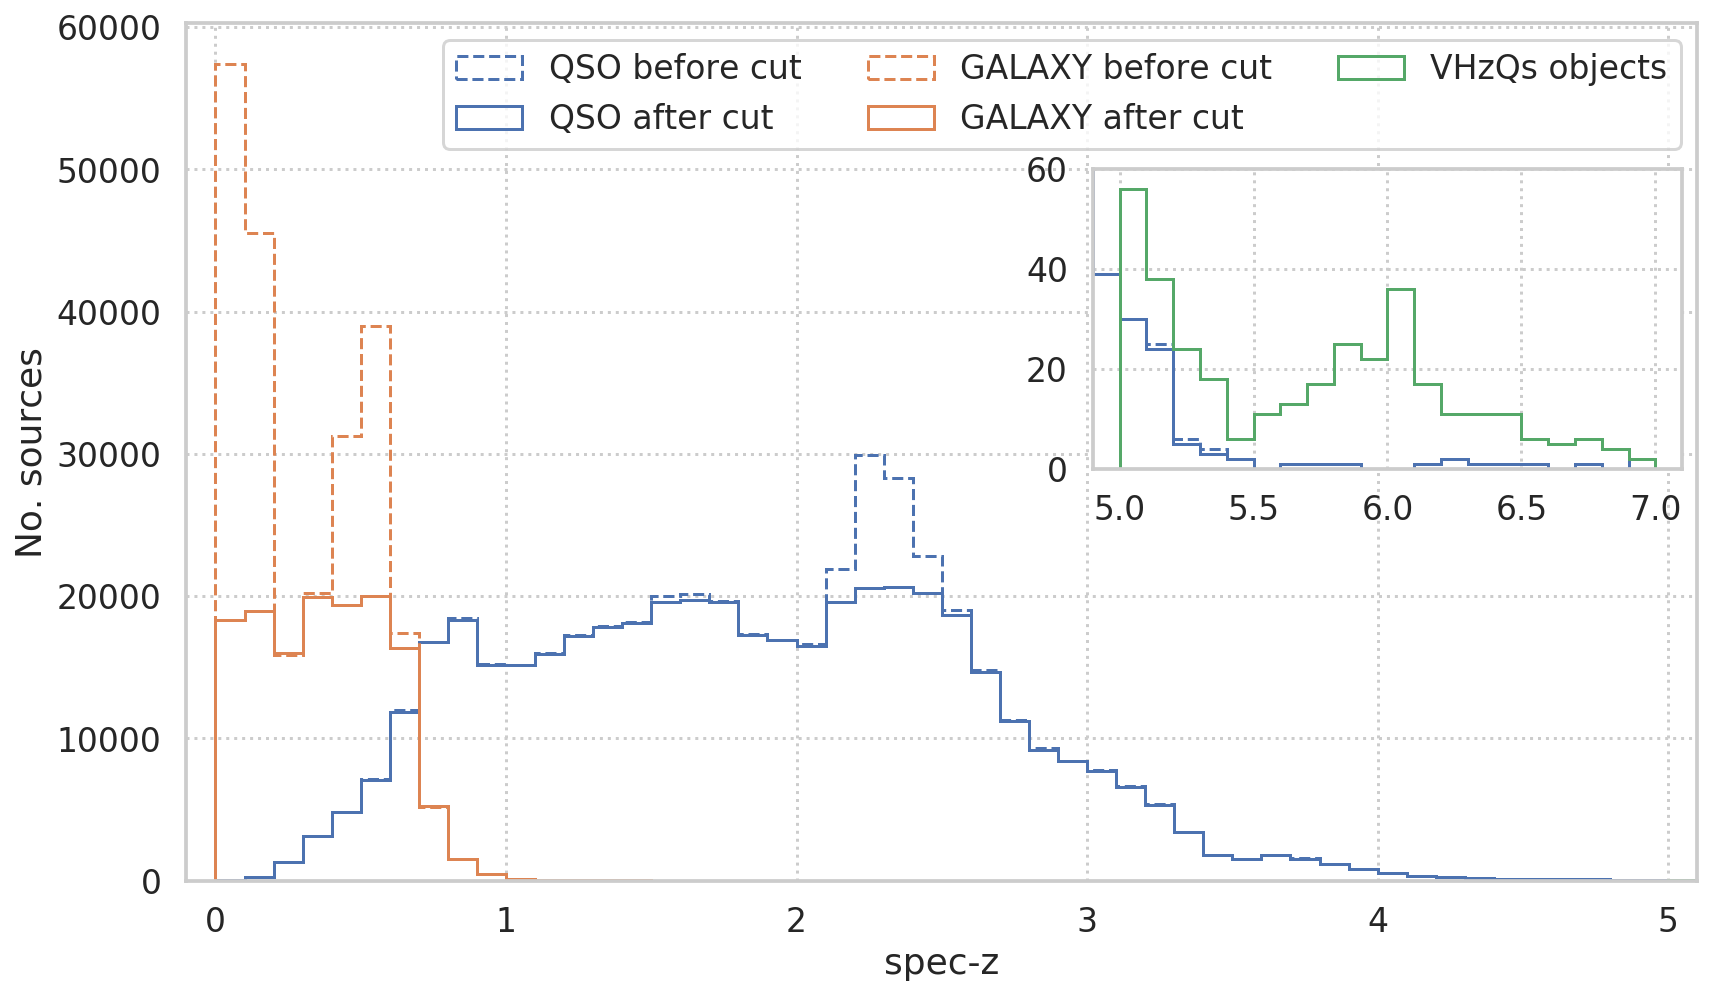
\includegraphics[width=0.95\linewidth]{images/train-peaks-cut.png}
    \caption{Обрезка пиков распределений тренировочной выборки. Обрезка пиков распределений галактик и кавзаров производилась независимо (гистограммы, показанные на графике тоже независимы). Цветом обозначен тип объектов (синий -- квазары, оранжевый -- галактики), штриховая линия - гистограмма распределения до обрезки, сплошная -- после.}
    \label{fig:train-peaks-cut}
\end{figure*}

\subsection{Stripe82X test sample}
Для тестирования моделей photo-z будут использоваться выборки тестовых полей Stripe82X и XMM-XXL-N. Выборка рентгеновских объектов области Stripe82X подробно описана в \cite{bib:ananna2017}. На данный момент эта выборка является самой крупной выборкой рентгеновских объектов, имеющих качественную классификацию по спектрам, и размеченных вручную, что делает её основной тестовой выборкой для сравнения моделей photo-z рентгеновских объектов. Данная выборка использовалась в качестве теста авторами двух вышеупомянутых моделей (SOTA) \cite{bib:ananna2017}, \cite{bib:brescia2018}. 
\subsection{Test sample of DR16q objects}
\begin{table*}
	\begin{tabular}{llllllll}
            \hline
            {}           & \multicolumn{3}{l}{No. sources}      & \multicolumn{4}{l}{With photometry from}  \\
             Sample      &       Total &     Galaxies &     QSO & DESI LIS & Pan-STARRS &    SDSS & All 3 surveys \\
            \hline
            Train        &      586176 &       136428 &  449748 &   580511 &     578815 &  578650 &  577049 \\
            Stripe82X    &        2909 &          648 &    1771 &     2898 &       2434 &    2862 &    2407 \\
            DR16q test   &       58682 &            0 &   58682 &    58447 &      50055 &   58366 &   49992 \\
            \hline
            \end{tabular}
            \caption{Описание используемых выборок (количество объектов по классам (галактики, квазары) и доли объектов, имеющих фотометрию в используемых широких обзорах неба). Поскольку кросс-отождествление сначала производится с каталогом DESI LIS, а потом для компаньонов DESI LIS ищутся данные Pan-STARRS и SDSS, доли объектов с фотометрией Pan-STARRS и SDSS не больше, чем с DESI LIS.}
\end{table*}

\begin{figure*}
    \centering
    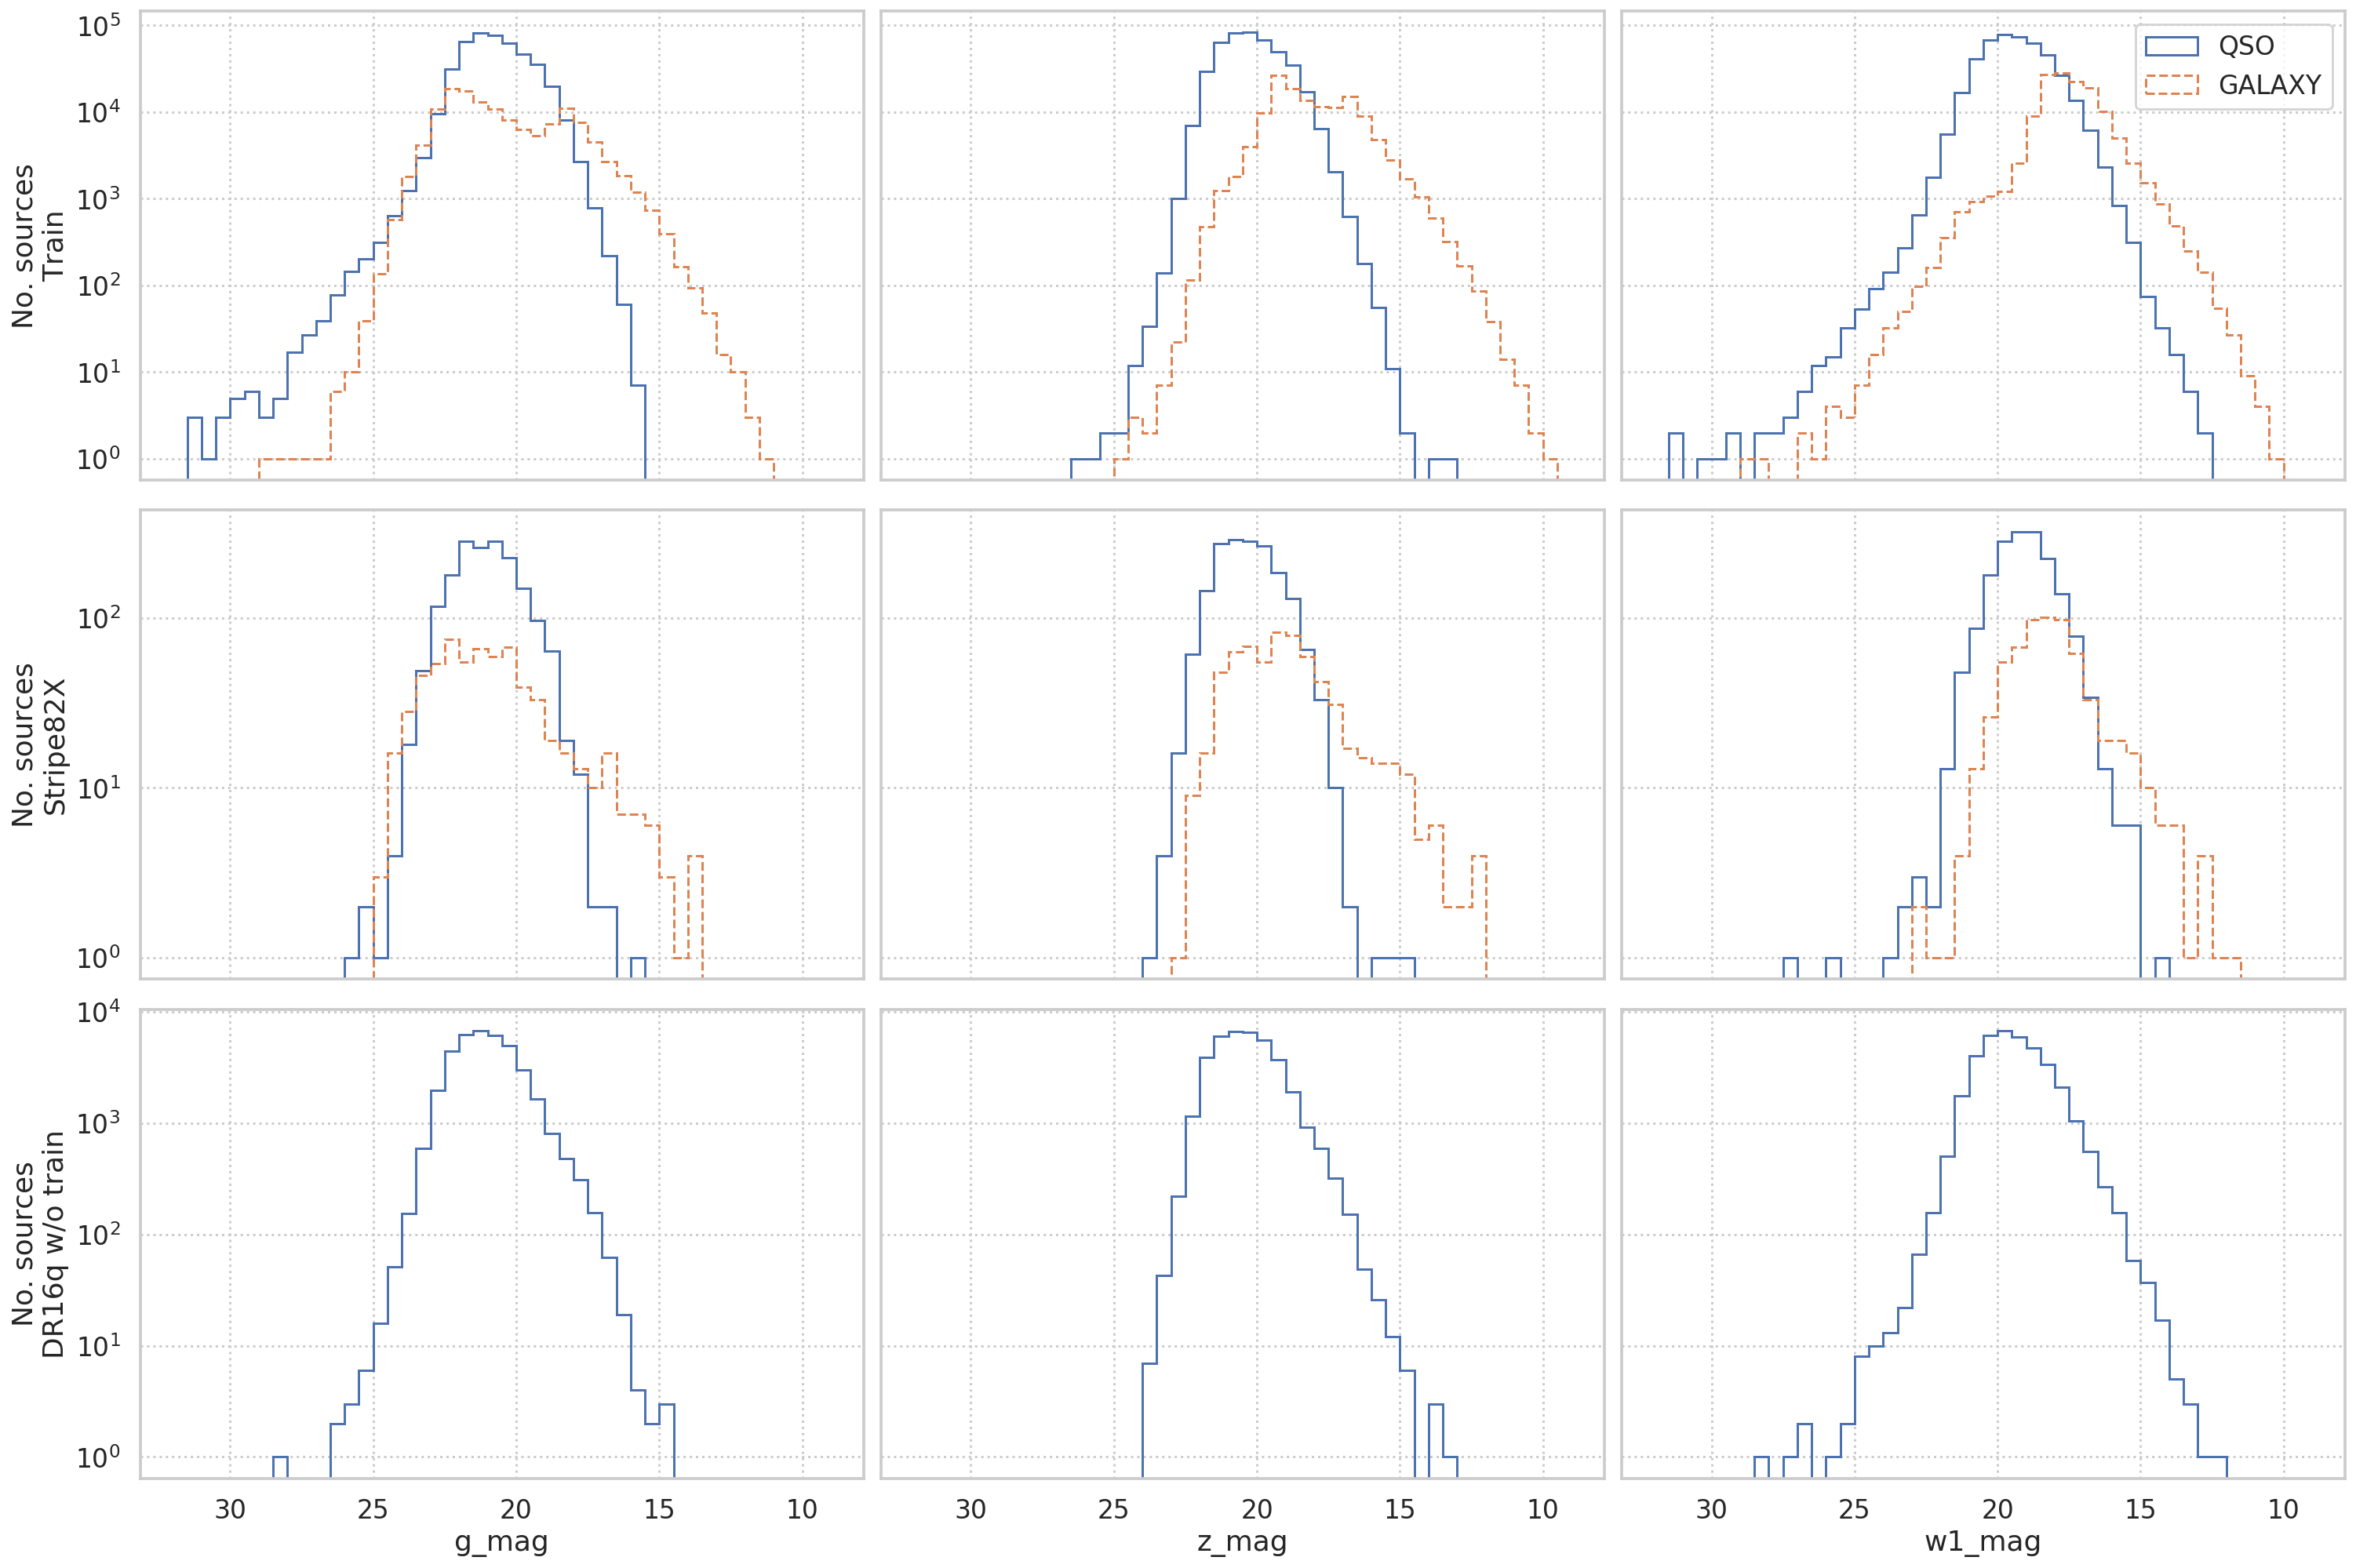
\includegraphics[width=0.9\linewidth]{images/data-dist-mags-ab.png}
    \caption{Гистограммы распределений объектов в выборках по величине \eqref{eq:mag_ab} в синем (g), красном (z) и инфракрасном (w1) фильтрах.}
    \label{fig:my_label}
\end{figure*}

\begin{figure*}
    \centering
    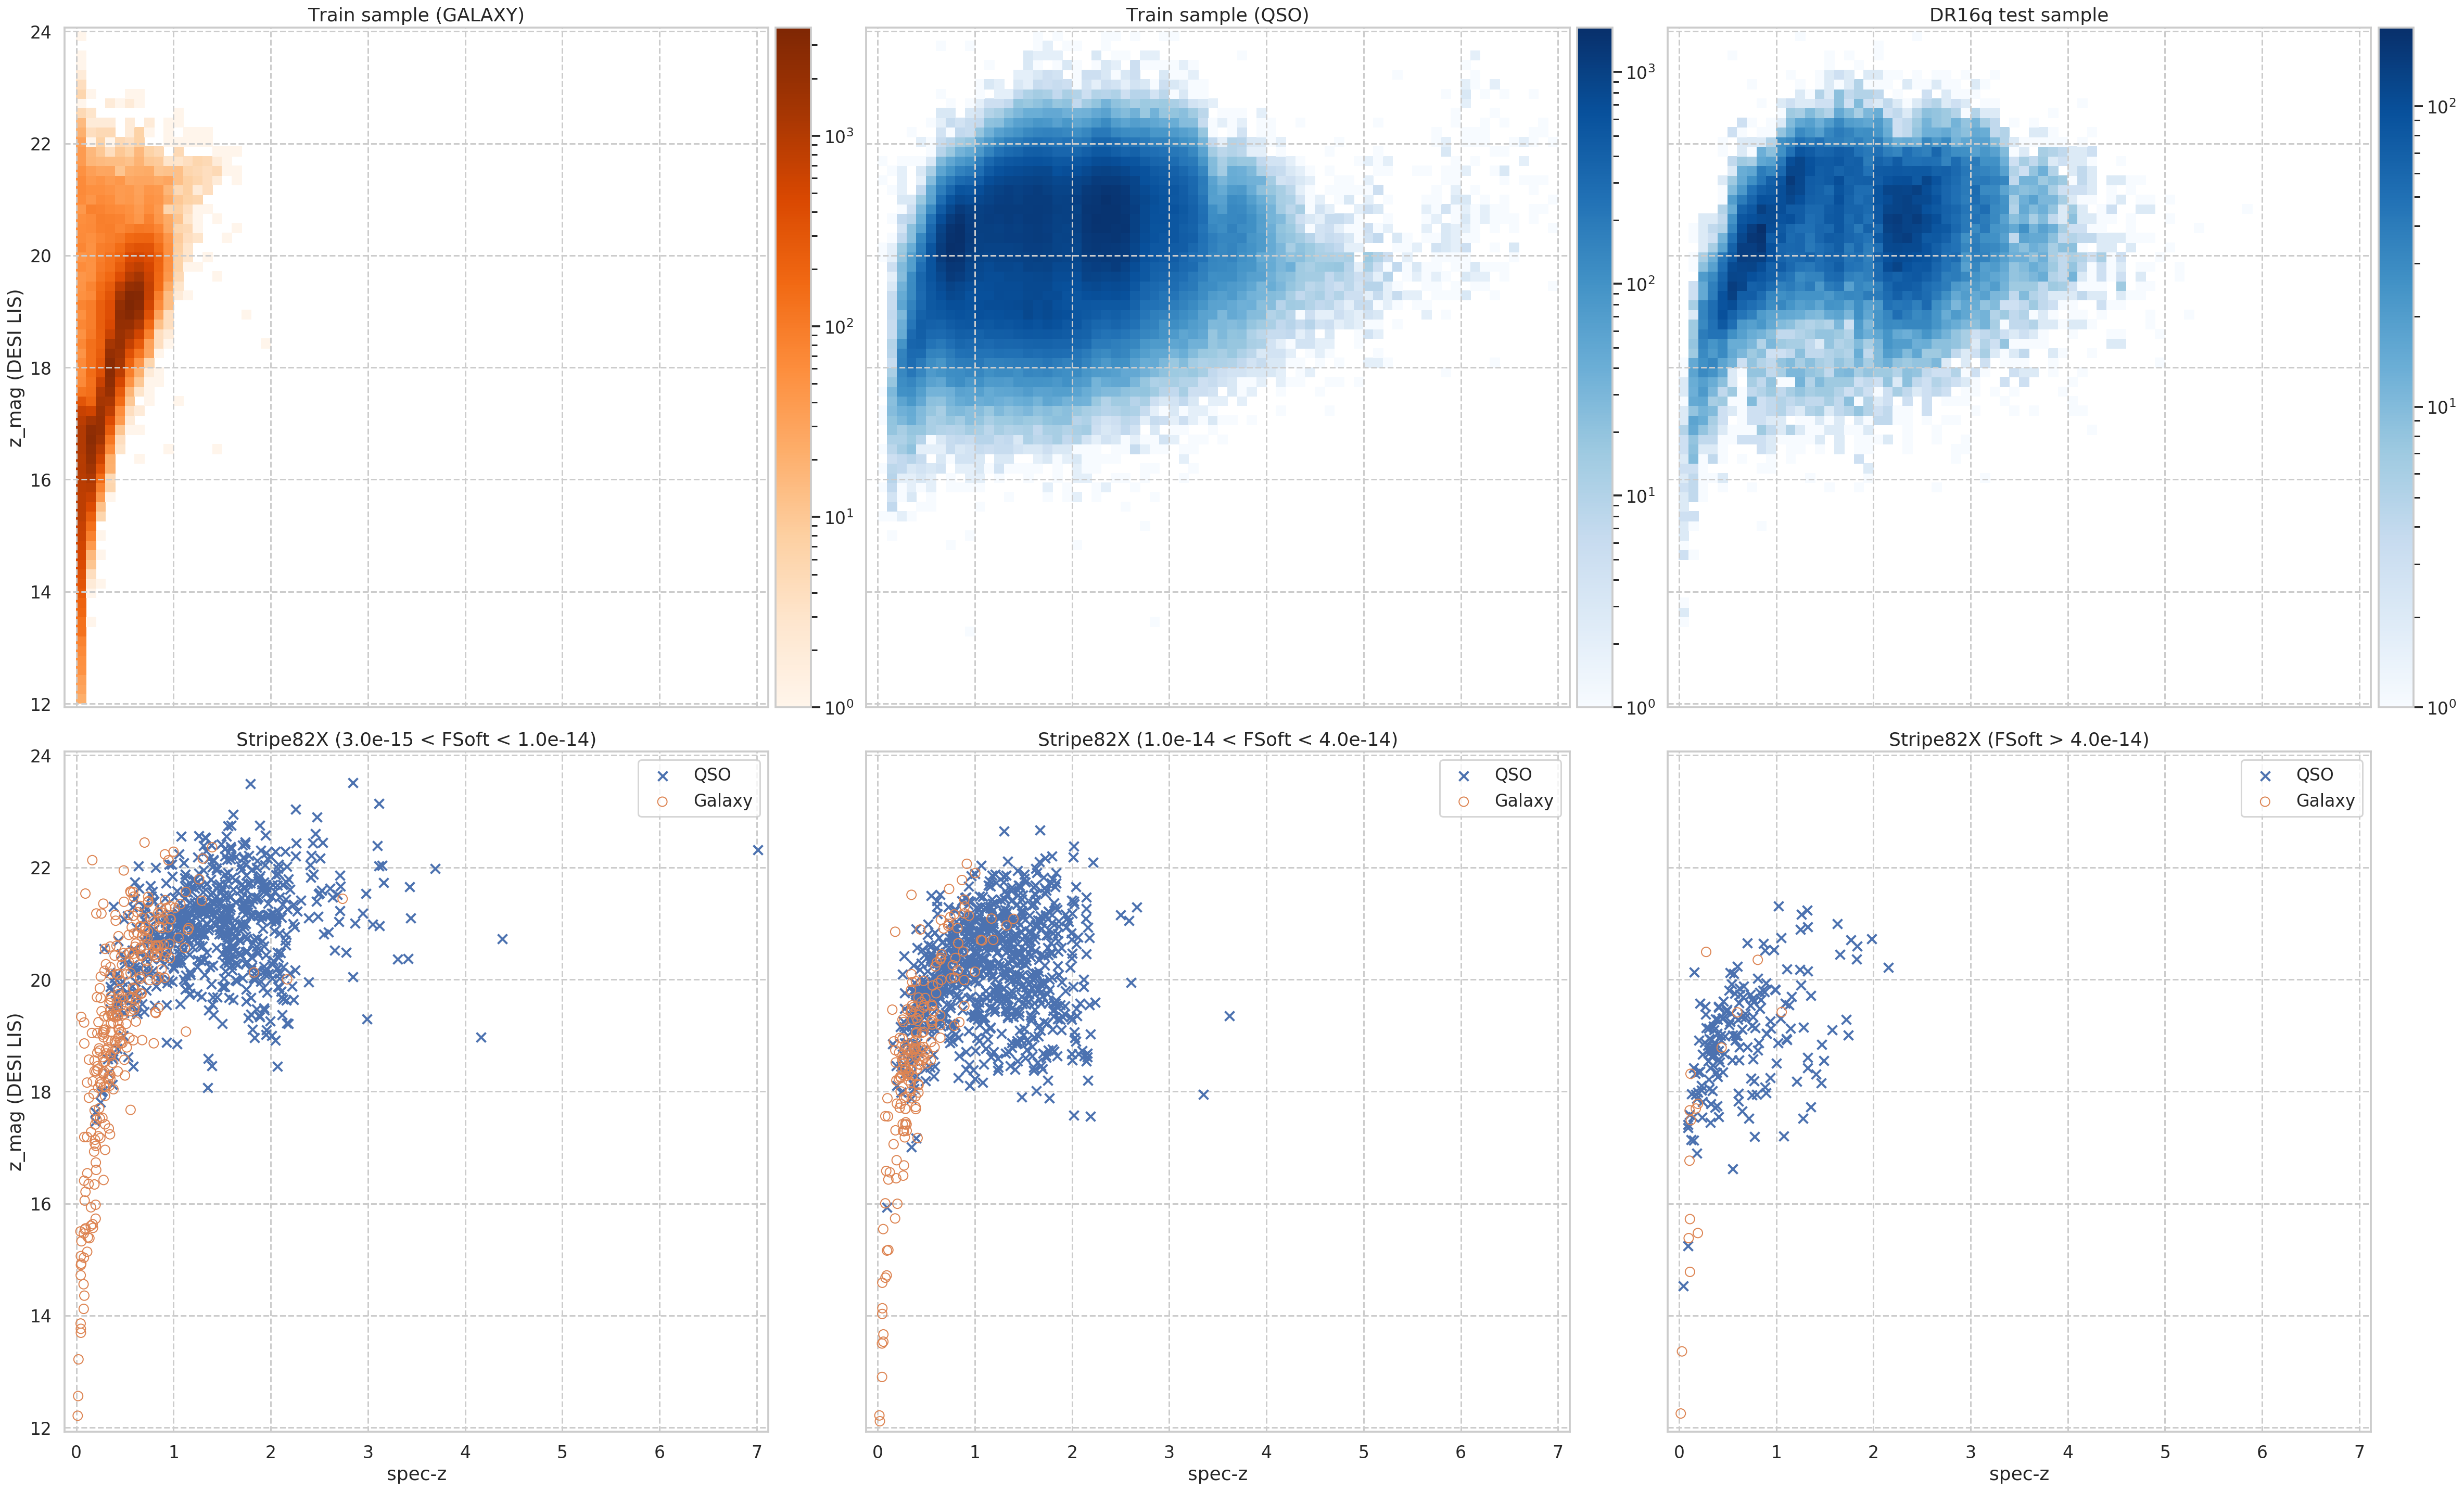
\includegraphics[width=0.95\linewidth]{images/data-dist-ab.png}
    \caption{Распределения объектов в используемых выборках. По оси абсцисс -- спектральное красное смещение, по оси ординат -- величина \eqref{eq:mag_ab} в фильтре $z$. Слева сверху -- объекты Stripe82X, оранжевыми крестиками показаны галактики, синими плюсиками -- квазары. Справа сверху -- двумерная гистограмма распределения объектов тестовой выборки квазаров SDSS DR16q. Снизу -- двумерные гисторгаммы распределения галактик (слева) и квазаров (справа) тренировочной выборки.}
    \label{fig:data_distribution}
\end{figure*}

% ===============================================================================
% ===============================================================================
% ===============================================================================

\section{The algorithm}

\subsection{Probabilistic regression}
Для постановки задачи вероятностной регрессии рассмотрим вероятностную постановку задачи регрессии. Пусть \(X\) - множество описаний объектов (пространство признаков), \(Y\) - область определения целевой переменной. Представим объекты и целевую переменную как случайные величины \(\xi : \Omega \rightarrow X, \eta : \Omega \rightarrow Y \). Тогда процесс, порождающий данные будет представлен как совместное распределение \((\xi, \eta) \sim p(x, y)\). Пусть дана обучающая выборка \(\mathcal{D}_n = (X_i, y_i)_{i=1}^n \sim p(x,y)\). Задача регрессии заключается в построении оценки условного среднего
\begin{equation}\label{eq:regr_classic}
     \hat{y} = \mathbb{E}[\eta | \xi = x] = \int_Y y ~ \hat{p}(y|x) ~ dy
\end{equation}

Для получения вероятностного прогноза вместо прогноза условного среднего необходимо построить прогноз условного распределения целевой величины \(\hat{p}(y|x)\), которое, формально, задает точечную оценку \eqref{eq:regr_classic}. Таким образом, задачей построения вероятностной регрессии является обучение оператора \(\hat{\eta} : X \rightarrow \mathcal{P} \subset L^2\)
\begin{equation}
    \hat{\eta}(x) = \hat{p}(y|x) \in \mathcal{P},
\end{equation}
где \(\mathcal{P}\) - множество ограниченных функций, удовлетворяющих свойствам функции плотности вероятности, то есть
\begin{equation}
    \forall p \in \mathcal{P}, y \in Y, x \in X \Rightarrow p(y|x) \geq 0,
\end{equation}
\begin{equation}
    \forall p \in \mathcal{P}, x \in X \Rightarrow \exists \int_{-\infty}^{+\infty} p(y|x) dy = 1.
\end{equation}
В идеальном случае при увеличении объема \(n\) обучающей выборки \(\mathcal{D}_n\) решение \(\hat{p}(y|x)\) задачи должно сходиться к функции плотности исходного порождающего процесса \(p(x|y) = \frac{p(x,y)}{p(x)}\). Однако, в явном виде порождающий процесс неизвестен: известны только тренировочная выборка \(\mathcal{D}_n\) и тестовая выборка, на которой будет оцениваться качество.

Критерии качества вероятностных прогнозов -- точность и калибровка -- подробно описаны в разделе \ref{sec:metrics}.

\subsection{Random forests for probabilistic photo-z}

\subsubsection{Random forests algorithm}
Алгоритм случайного леса для решения задач регрессии классификации был впервые описан в \citep{2001MachL..45....5B} и представляет собой ансамбль деревьев решений $\{A^j\}$, которые строятся независимость. Прогноз случайного леса получается аггрегацией прогнозов всех деревьев. Например, для задачи регрессии итоговый прогноз равен среднему прогнозов деревьев.

Каждое дерево $A^j$ строит разбиение пространства признаков $X$ на непересекающиеся подпространства $A^j_i$, которые в сумме дают все пространство, то есть
\begin{equation}
    \sum_i A^j_i = X, A^j_n \cap A^j_m = \emptyset, m \neq n.
\end{equation}

Построение модели на основе алгоритма случайного леса производится следующим образом. Пусть дана обучающая выборка размера $N$:
\begin{equation}\label{eq:train_sample}
    \mathcal{D} = (\mathcal{D}_X, \mathcal{D}_y),
\end{equation}
\begin{equation}\label{eq:train_features}
    \mathcal{D}_X = (x_{i,j})_{j=1}^M,
\end{equation}
\begin{equation}\label{eq:train_target}
    \mathcal{D}_y = (y_i),
\end{equation}
где $\mathcal{D}_X$ и $\mathcal{D}_y$ признаки и разметка объектов обучающей выборки, соответственно; $i=\overline{1, N}$. Для построения очередного дерева:
\begin{itemize}
    \item бутстрепом генерируется случайная подвыборка $\mathcal{D}^j$ обучающей выборки \eqref{eq:train_sample},
    \item при каждом разбиении в $j$-ом дереве случайно выбираются случайные $m$ признаков из \eqref{eq:train_features}, $m < M$,
    \item для очередного разбиения по заданному критерию определяются оптимальный из $m$ отобранных признаков и пороговое значение,
    \item разбиения строятся пока не исчерпается вся выборка $\mathcal{D}^j$ (дерево без ограничения глубины) или до выполнения определенного условия (в каждом листе осталось не более $n_{min} \in \Theta$ объектов или достигнута заданная высота дерева $h_{max} \in \Theta$.
\end{itemize}

Впервые для задачи вероятностной регрессии был использован в работе \cite{JMLR:v7:meinshausen06a} для точечной оценки квантилей. Построение модели заключается в обучении случайного леса с квантильной функцией потерь 
\begin{equation}\label{eq:quantile_loss}
    l(y_i, \hat{q}_{\alpha, i}) = (1-\alpha)|y_i - \hat{q}_{\alpha, i}|\mathbb{I}[y_i \leq \hat{q}_{\alpha, i}] + \alpha|y_i - \hat{q}_{\alpha, i}|\mathbb{I}[y_i > \hat{q}_{\alpha, i}],
\end{equation}
% \begin{equation}\label{eq:quantile_loss}
%     l(y_i, \hat{q}_{\alpha, i}) = \left\{\begin{array}{rcl}
%          \alpha|y_i - \hat{q}_{\alpha, i}| & y_i > \hat{q}_{\alpha, i} \\
%          (1-\alpha)|y_i - \hat{q}_{\alpha, i}| & y_i \leq \hat{q}_{\alpha, i}
%     \end{array}\right.,
% \end{equation}
где $y_i$ - истинное значение, $\hat{q}_{\alpha, i}$ - предсказанное значение квантиля заданного уровня значимости $\alpha$.

(Дописать критерии разбиения!)

В работе \ref{} проводится анализ поведения случайного леса при различных параметрах рандомизации. Функцию потерь можно разложить на 2 составляющие (так называемый Bias-Variance-Tradeoff:
\begin{equation}\label{eq:bias-variance-tradeoff}
    L = Bias + Variance,
\end{equation}.
Сами по себе деревья решений являются несмещенными $Bias = 0$, но имеют высокий Variance. Путем усреднения ансамбля прогнозов удается понизить Variance.

\subsection{Случайный лес как обобщенный метод ближайших соседей}

\subsubsection{TPZ}
(Проверить!) Для задачи прогноза photo-z впервые был применен в работе \cite{bib:tpz}. Авторы предлагают 2 варианта своего метода: режим классификации и режим регрессии. В обоих режимах область определения целевого признака разбивается на конечное количество непересекающихся интервалов $[y_j, y_{j+1}]$.

В режиме классификации вероятностный прогноз строится как набор вероятностей $\hat{p}_i$ того, что целевой признак заданного объекта принадлежит тому или иному интервалу значений:
\begin{equation}
    \hat{p}_j = \mathbb{P}(y_j \leq y_i < y_{j+1}).
\end{equation}
Для каждого интервала $[y_j, y_{j+1}]$ строится модель двуклассовой классификации на основе алгоритма случайного леса, которая предсказывает вероятность $\hat{p}_j$.

В режиме регрессии производится построение одной модели регрессии на основе алгоритма случайного леса. Оценка распределения получатся нормализацией количества объектов, прогнозы которых попали в интервалы $[y_j, y_{j+1}]$.

\subsection{Random Forests adoptation for probabilistic photo-z via Gaussian KDE}
В работе \cite{bib:mesch} сравниваются модели вероятностных photo-z оптических квазаров на основе случайного леса и на основе градиентного бустинга. Случайный лес без ограничения глубины был адаптирован для вероятностных прогнозов путем применения ядерной оценки плотности с гауссовым ядром
\begin{equation}\label{eq:gaussian_kernel}
    K(x) = \frac{1}{\sqrt{2\pi}} * \exp{(-\frac{1}{2} x^2)}.
\end{equation}
к ансамблю прогнозов деревьев. Таким образом прогноз представляет собой параметрическую оценку плотности условного распределения:
\begin{equation}\label{eq:kde}
    \hat{p}_i (y) = \hat{p}(y|x_i) = \frac{1}{n_{trees} h}\sum_{j=1}^{n_{trees}} K(\frac{y - \hat{y^{(j)}_i}}{h}),
\end{equation}
где $h$ -- параметр ширины ядра.

Данный подход имеет следующую теоретическую интерпретацию: независимость и случайность построения деревьев позволяет рассматривать ансамбль прогнозов деревьев $\{y^j_i\}_{i=1}^{n_{trees}}$ как случайную выборку, порожденную истинным распределением $p(y|x_i)$. Таким образом \eqref{eq:kde} является оценкой этого распределения.

В отличие от случайного леса, каждое следующее дерево в градиентном бустинге строится на основе предыдущего, что не позволяет применить подход, описанный выше. Вместо модели обучались с квантильной функцией пртерь \eqref{eq:quantile_loss} для разных уровней значимости $\alpha$, и производится прогноз набора квантилей.

По результатам сравнения, проведенного в статье, подход на основе случайного леса показал точность выше градиентного бустинга.

% Случайный лес \cite{bib:forests_brieman} представляет собой ансамбль деревьев, основанных на одном и том же базовом алгоритме построения дерева решений, которые строятся на случайных подвыборках одной тренировочной выборки. Каждое дерево \(A^j\) задает разбиение признакового пространства \(X\) на не пересекающиеся прямоугольные подпространства \(A^j_i\), соответствующие листьям дерева, то есть
% \begin{equation}
%     X = \bigcup_i {A^j_i}; A^j_n \cap A^j_m = \emptyset, n \neq m.
% \end{equation}
% При этом каждое дерево содержит в себе некоторую случайность построения, которая контролируется вектором гиперпараметров случайного леса \(\Theta\). Например, \(\Theta\) может задавать, по какому признаку и по какому диапазону его значений будет разбиваться очередной узел. Очень важным, что будет показано ниже, является параметр, контролирующий разбиение обучающей выборки на случайные подвыборки для построения деревьев. Таким образом, деревья, входящие в случайный лес получаются разными. Для получения финального прогноза прогнозы всех деревьев усредняются, т.е., обозначив случайный лес как ансамбль деревьев \(\mathbb{V}_T = \{A^j, 1 \leq j \leq T\}\), можно записать в виде формулы
% \begin{equation}
%     \hat{\eta}_{n, \mathbb{V}_T}(x) = \frac{1}{T} \sum_{j=1}^T \hat\eta_{n, A^j}(x),
% \end{equation}
% где \(\hat\eta_{n, A^j}(x)\) - прогноз дерева \(A^j\).

% Впервые для задачи вероятностной регрессии был использован в работе Meinshausen, 2006 \cite{bib:forests_meinshausen} для точечной оценки квантилей. Построение модели заключается в обучении случайного леса с квантильной функцией потерь 
% \begin{equation}
%     l(y_i, \hat{y}_{\alpha, i}) = (1-\alpha)|y_i - \hat{y}_{\alpha, i}|\mathbb{I}[y \leq \hat{y}_{\alpha, i}] + \alpha|y_i - \hat{y}_{\alpha, i}|\mathbb{I}[y > \hat{y}_{\alpha, i}],
% \end{equation}
% где \(y_i\) - истинное значение, \(\hat{y}_{\alpha, i}\) - предсказанное значений целевой переменной.

% Для задачи прогноза photo-z впервые был применен в работе \cite{bib:tpz}, где вероятностный прогноз строится как набор вероятностей того, что целевой признак заданного объекта принадлежит тому или иному интервалу значений. В работе \cite{bib:mesch} вероятностный прогноз представляет собой непрерывную функцию плотности вероятности, полученную применением ядерной оценки плотности к ансамблю прогнозов деревьев. Важно заметить, что в обоих алгоритмах используются леса, без ограничения глубины, т.е. когда в каждом листе каждого дерева находится один и только один элемент тренировочной выборки. 

\subsection{Random forest adoptation for probabilistic predictions}
Our aim was to estimate conditional redshift distribution $p(z|x)$ for each target object with photometric features $x$.
We use Random Forest (RF) model, \citep{2001MachL..45....5B,JMLR:v7:meinshausen06a}, which is considered by many authors among the most accurate ML algorithms for photo-z measurements of galaxies \citep{2020MNRAS.499.1587S,2020arXiv200912112E} and X-ray quasars \citep{2018AstL...44..735M}. We used RF ensemble predictions in combination with gaussian Kernel Density Estimation (gKDE), to obtain $p(z|x)$. RF+gKDE model allows one to calculate photo-z point estimate $\hat{z}_{ph} = \arg\max_z p(z|x)$, confidence intervals, and $zConf = \int_{\delta z_{norm} < 0.06} p(z|x)~dz$.

At the prediction stage we take into account uncertainties in photometric fluxes of the target object, by perturbing  fluxes (according to given uncertainties) for each regression tree in the forest. Схема используемаого метода представлена на рисунке \ref{fig:qrf_scheme}.

\begin{figure}
    \centering
    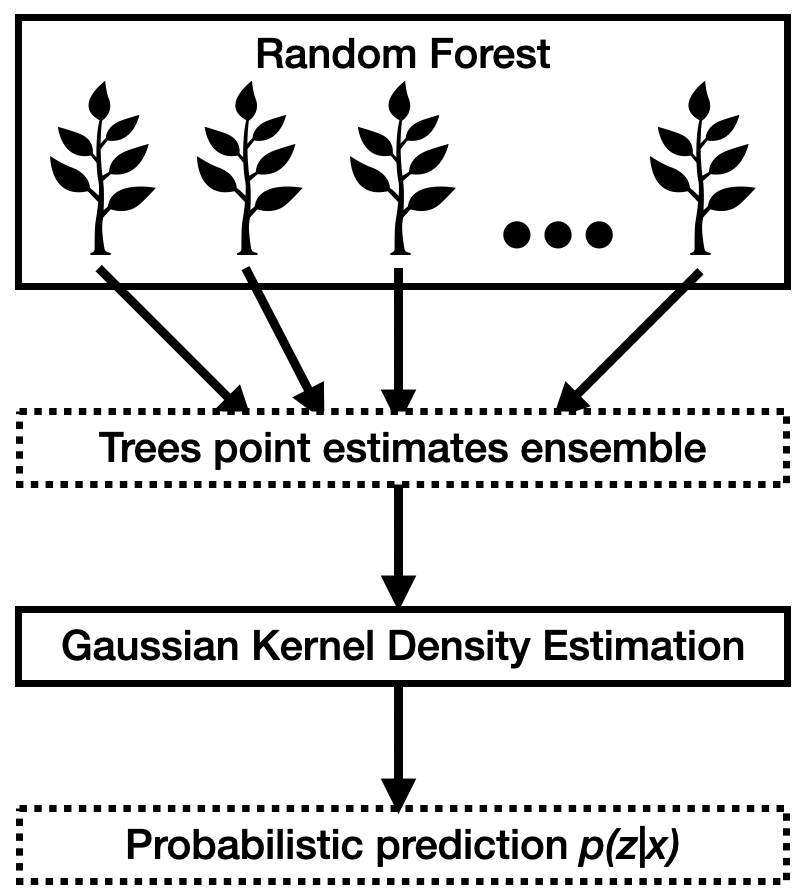
\includegraphics[width=0.95\linewidth]{images/qrf.png}
    \caption{Схема используемого алгоритма случайного леса, адоптированного для получения вероятностных прогнозов photo-z.}
    \label{fig:qrf_scheme}
\end{figure}

\section{Metrics}\label{Критерии качества вероятностных прогнозов}

Вероятностные прогнозы имеют 2 критерия качества -- точность точечных прогнозов и калибровка (соответствие предсказанного распределения реальному).

В данном разделе описываются метрики качества прогнозов. В разделе \ref{sec:point-metrics} описаны метрики точечных прогнозов, разделе \ref{sec:calibration-metrics} -- метрики калибровки доверительных интервалов и полных вероятностных прогнозов. В разделе \ref{sec:quality-confllict} дается обоснование конфликтности точности и калибровки.

\subsection{Point-estimates metrics}\label{sec:point-metrics}

Чтобы оценить качество точечных прогнозов photo-z, полученных из вероятностного прогноза, мы используем 2 метрики стандартные для задачи прогнозов photo-z:
\begin{itemize}
    \item Оценка колокола распределения ошибок \begin{equation}\label{eq:nmad}
        NMAD = 1.4826 \times median(|\delta z_{norm,i}|)
    \end{equation}
    \item и долю катастрофических выбросов \begin{equation}\label{eq:n015}
        n_{>0.15} = \frac{\#\{i = \overline{1, N} | \delta z_{norm, i} > 0.15\}}{N};
    \end{equation}
\end{itemize}
где \(N\) - размер выборки, и ошибка прогноза \begin{equation}\label{eq:dznorm}
    \delta z_{norm,i} = \frac{\Delta z_i}{1+z_{spec,i}} = \frac{\hat{z}_{ph,i} - z_{spec,i}}{1+z_{spec,i}}.
\end{equation}

\subsection{Метрики калибровки}\label{sec:calibration-metrics}

Метрики калибровки можно разделить на 2 типа: калибровка доверительных интервалои и калибровка распределений.

Для оценки качества калибровки доверительных интервалов можно сравнивать теоретический фактический уровень доверия 68-процентных доверительных интервалов:
\begin{equation}\label{eq:calpha}
    C_{\alpha} = \frac{\#\{i = \overline{1, N} | z_{ph,i} \in CI_{\alpha, i}\}}{N}.
\end{equation}
При идеальной калибровке будет достигаться равенство
\begin{equation}\label{eq:perfect-ci}
    C_{\alpha} = \alpha ~ \forall \alpha \in [0, 1]
\end{equation}

В этой работе мы будем оценивать калибровку 68-процентных доверительных интервалов:
\begin{equation}\label{eq:c68}
    C_{68} - 0.68 = \frac{\#\{i = \overline{1, N} | z_{ph,i} \in CI_{68, i}\}}{N} - 0.68.
\end{equation}
При хорошей калибровке доверительных интервалов 

Для оценки качества калибровки распределений может быть использовано вероятностное интегральное преобразование (англ. Probability Inntegral Transform, PIT), которое вычисляется для каждого объекта выборки по формуле

\begin{equation}\label{eq:pit}
PIT_i = \hat{F}_i(y_{true}); \hat{F}_i(y) = \int_{-\infty}^{y} \hat{p}_i(y|x) ~ dy
\end{equation}

При идеальной калибровке распределений PIT-значения имеют равномерное распределение на отрезке \([0,1]\), что позволяет использовать гистограмму PIT-значений или квантильный график для визуальной оценки качества (для выборки качественных прогнозов ожидается ровная гистограмма). Пример PIT-гистограммы и квантильного графика для распределений представлены на рис. \ref{img:pitqq} слева. Квантильный график представляет собой, в некотором роде, интегральную гистограмму PIT-значений. Большое количество слишком широких вероятностных прогнозов (распределений) повлечет за собой большое количество PIT значений около 0.5 и выпуклую гистограмму, что является признаком "неуверенности" модели (underconfidence). Наоборот, большое количество слишком узких распределений влечет вогнутую гистограмму, что является признаком "чрезмерной уверенности" модели (overconfidence), при этом большое количество PIT значений около 0 или около 1 свидетельствуют о большом количестве катастрофических выбросов. Тогда долю катастрофических выбросов, можно определить как доля PIT-значений меньше \(0,001\) и больше \(1-0.001\) Кроме того, в качестве метрики можно использовать метрику Колмогорова-Смирнова, которое является расстоянием между кумулятивной функцией распределения полученных PIT-значений \(F_{PIT}(x)\) (оно же, суть, квантильный график) и кумулятивной функцией распределения, описывающей идеальную калибровку, \(F_{ideal}(X)\) на отрезке \([0,1]\):

\begin{equation}\label{eq:kspit}
    KS_{PIT} = \max_{x \in [0,1]}(F_{PIT}(x), F_{ideal}(x))
\end{equation}{}

\begin{equation}
    F_{PIT}(x) = \frac{\#[PIT_i < x, i=\overline{1,n}]}{N}; ~ F_{ideal} = x\mathbb{I}[0 < x \leq 1] + \mathbb{I}[x > 1]
\end{equation}{}

\subsection{Конфликт точности и калибровки}\label{sec:quality-conflict}
Критерии качества вероятностных прогнозов -- точность и калибровка -- не могут быть достигнуты одновременно. Это демонстрируется на двух dummy-моделях.

Представим, что в качестве прогноза возвращается истинное значение целевого признака. Тогда фактический уровень доверия доверительных интервалов \eqref{eq:calpha} будет равен 1 для любых значений уровня доверия $\alpha$. Все PIT-значения так же будут равны 1.

С другой стороны можно представить пример, когда в качестве прогноза для любого объекта возвращается распределение объектов по целевому признаку в целевй выборке. В данном случае будет достигаться равенство \eqref{eq:perfect-ci}, а PIT-значения будут иметь равномерное распределение на отрезке [0, 1]. Однако точность такой модели будет весьма посредственной.

% В качестве метрики распределений будет использоваться калибровка меры достоверности прогноза \(zConf\) \eqref{}, которая имеет смысл вероятности. Для неё будет оцениваться кумулятивная функция распределения \begin{equation}\label{eq:zconf_cal}
%     F(x) = \frac{\#\{i = \overline{1, N} | zConf_i < x \}}{N}.
% \end{equation}
% При хорошей калибровке мы рассчитываем увидеть функцию равномерного распределения на интервале $[0, 1]$. Контролировать калибровку меры уверенности прогноза $zConf$ очень важно, поскольку она используется для отбора кандидатов в наиболее далекие квазары.



% ===============================================================================
% ===============================================================================
% ===============================================================================

\section{Results}
Пример ссылки на строку из таблицы \ref{tab:models} -- строка \ref{model:spdw} описывает нашу топовую модель, a строка \ref{model:pw} -- модель на всем небе. Все они используют признаки WISE (см. таблицу \ref{tab:featuressets}, строки \ref{feats:wise-mags-1}).

Нашей целью является исследование поведения моделей, построенных на разных наборах признаков (прдробнее см. в \ref{}), в зависимости от наблюдаемых предикторов (величины в фильтрах r, z, рентгеновский поток) и от целевой величины (spec-z). Чтобы добиться лучшего разрешения (это особенно актуально для объектов на $z > 3$) мы используем метод двукратной перекрестной оценки и выборку оптических квазаров SDSS DR16q, описанную в разделе \ref{}. Эти наблюдения описаны в разделе \ref{subsec:cv2_results} и \ref{subsec:dr16_results}, соответственно.

В разделе \ref{subsec:s82x_results} такие же наблюдения на выборке рентгеновских объетов Stripe82X, описанной в разделе \ref{}. На этой же выборке мы приводим сранение с прогнозами моделей SOTA \ref{}.

\subsection{Результаты на кросс-валидации (галактики)}

% \begin{figure*}
%     \centering
%     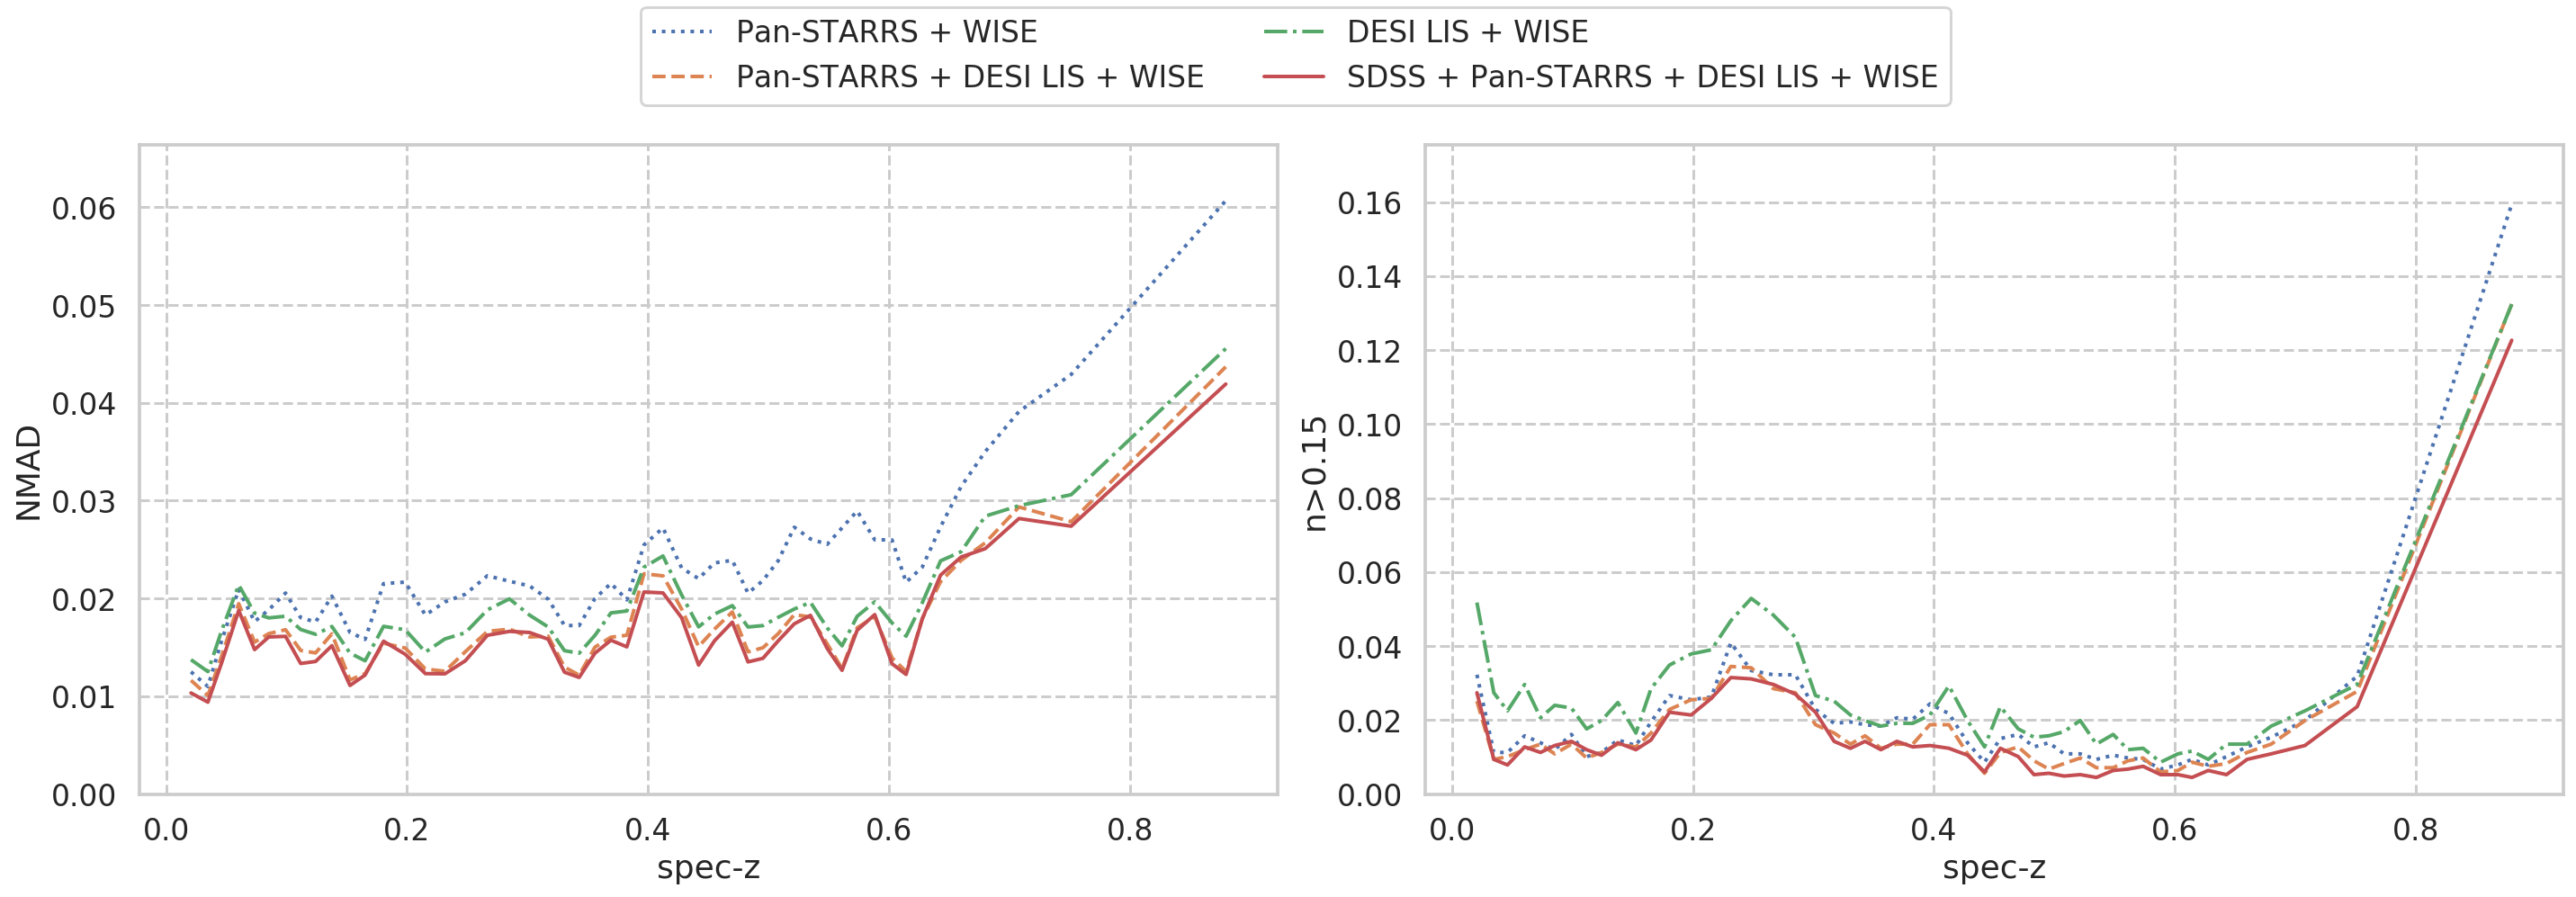
\includegraphics[width=0.9\linewidth]{images/metrics-gal_spec-z.png}
%     \caption{Графики метрик точности моделей в зависимости от значения spec-z. На верхних графиках показана метрика $NMAD$ \eqref{eq:nmad}, на нижних графиках -- доля катастрофических выбросов $n_{>0.15}$ \eqref{eq:n015}. Слева -- метрики на двукратной кросс-валидации, справа -- на тестовой выборке оптических квазаров. Модели: Pan-STARRS + WISE -- синий пунктир, DESI LIS + WISE -- зеленый штрих-пунктир, Pan-STARRS + DESI LIS + WISE -- оранжевый штрих, SDSS + DESI LIS + WISE -- красная сплошная кривая.}
%     \label{fig:metrics-qso_spec-z}
% \end{figure*}

% \begin{figure*}
%     \centering
%     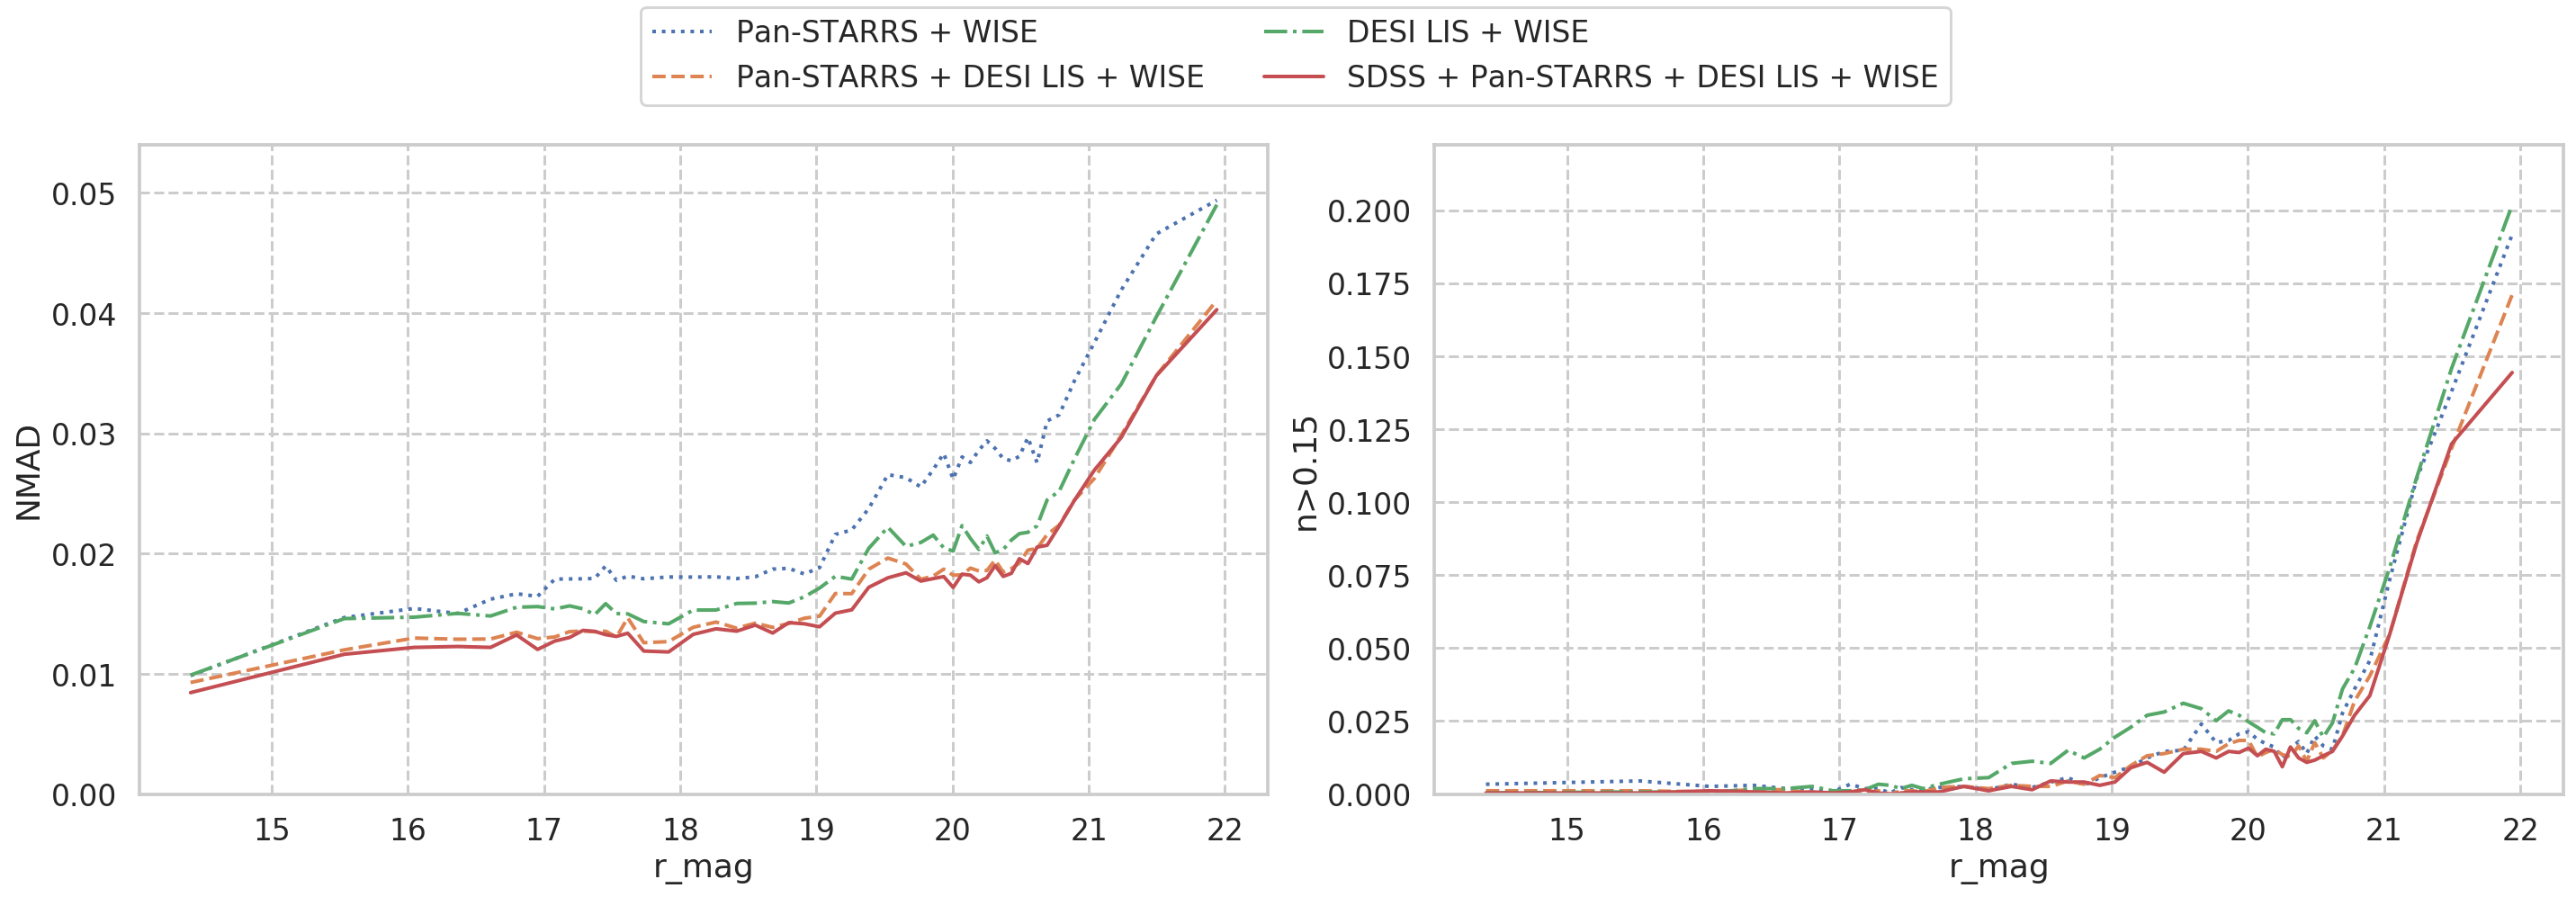
\includegraphics[width=0.9\linewidth]{images/metrics-gal_r-mag.png}
%     \caption{Графики метрик точности моделей в зависимости от значения величины $r$, посчитанной из потоков каталога DESI LIS по формуле гиперболического синуса \eqref{eq:asinhmag}. На верхних графиках показана метрика $NMAD$ \eqref{eq:nmad}, на нижних графиках -- доля катастрофических выбросов $n_{>0.15}$ \eqref{eq:n015}. Слева -- метрики на двукратной кросс-валидации, справа -- на тестовой выборке оптических квазаров. Модели: Pan-STARRS + WISE -- синий пунктир, DESI LIS + WISE -- зеленый штрих-пунктир, Pan-STARRS + DESI LIS + WISE -- оранжевый штрих, SDSS + DESI LIS + WISE -- красная сплошная кривая.}
%     \label{fig:metrics-qso_z_mag}
% \end{figure*}

% \begin{figure*}
%     \centering
%     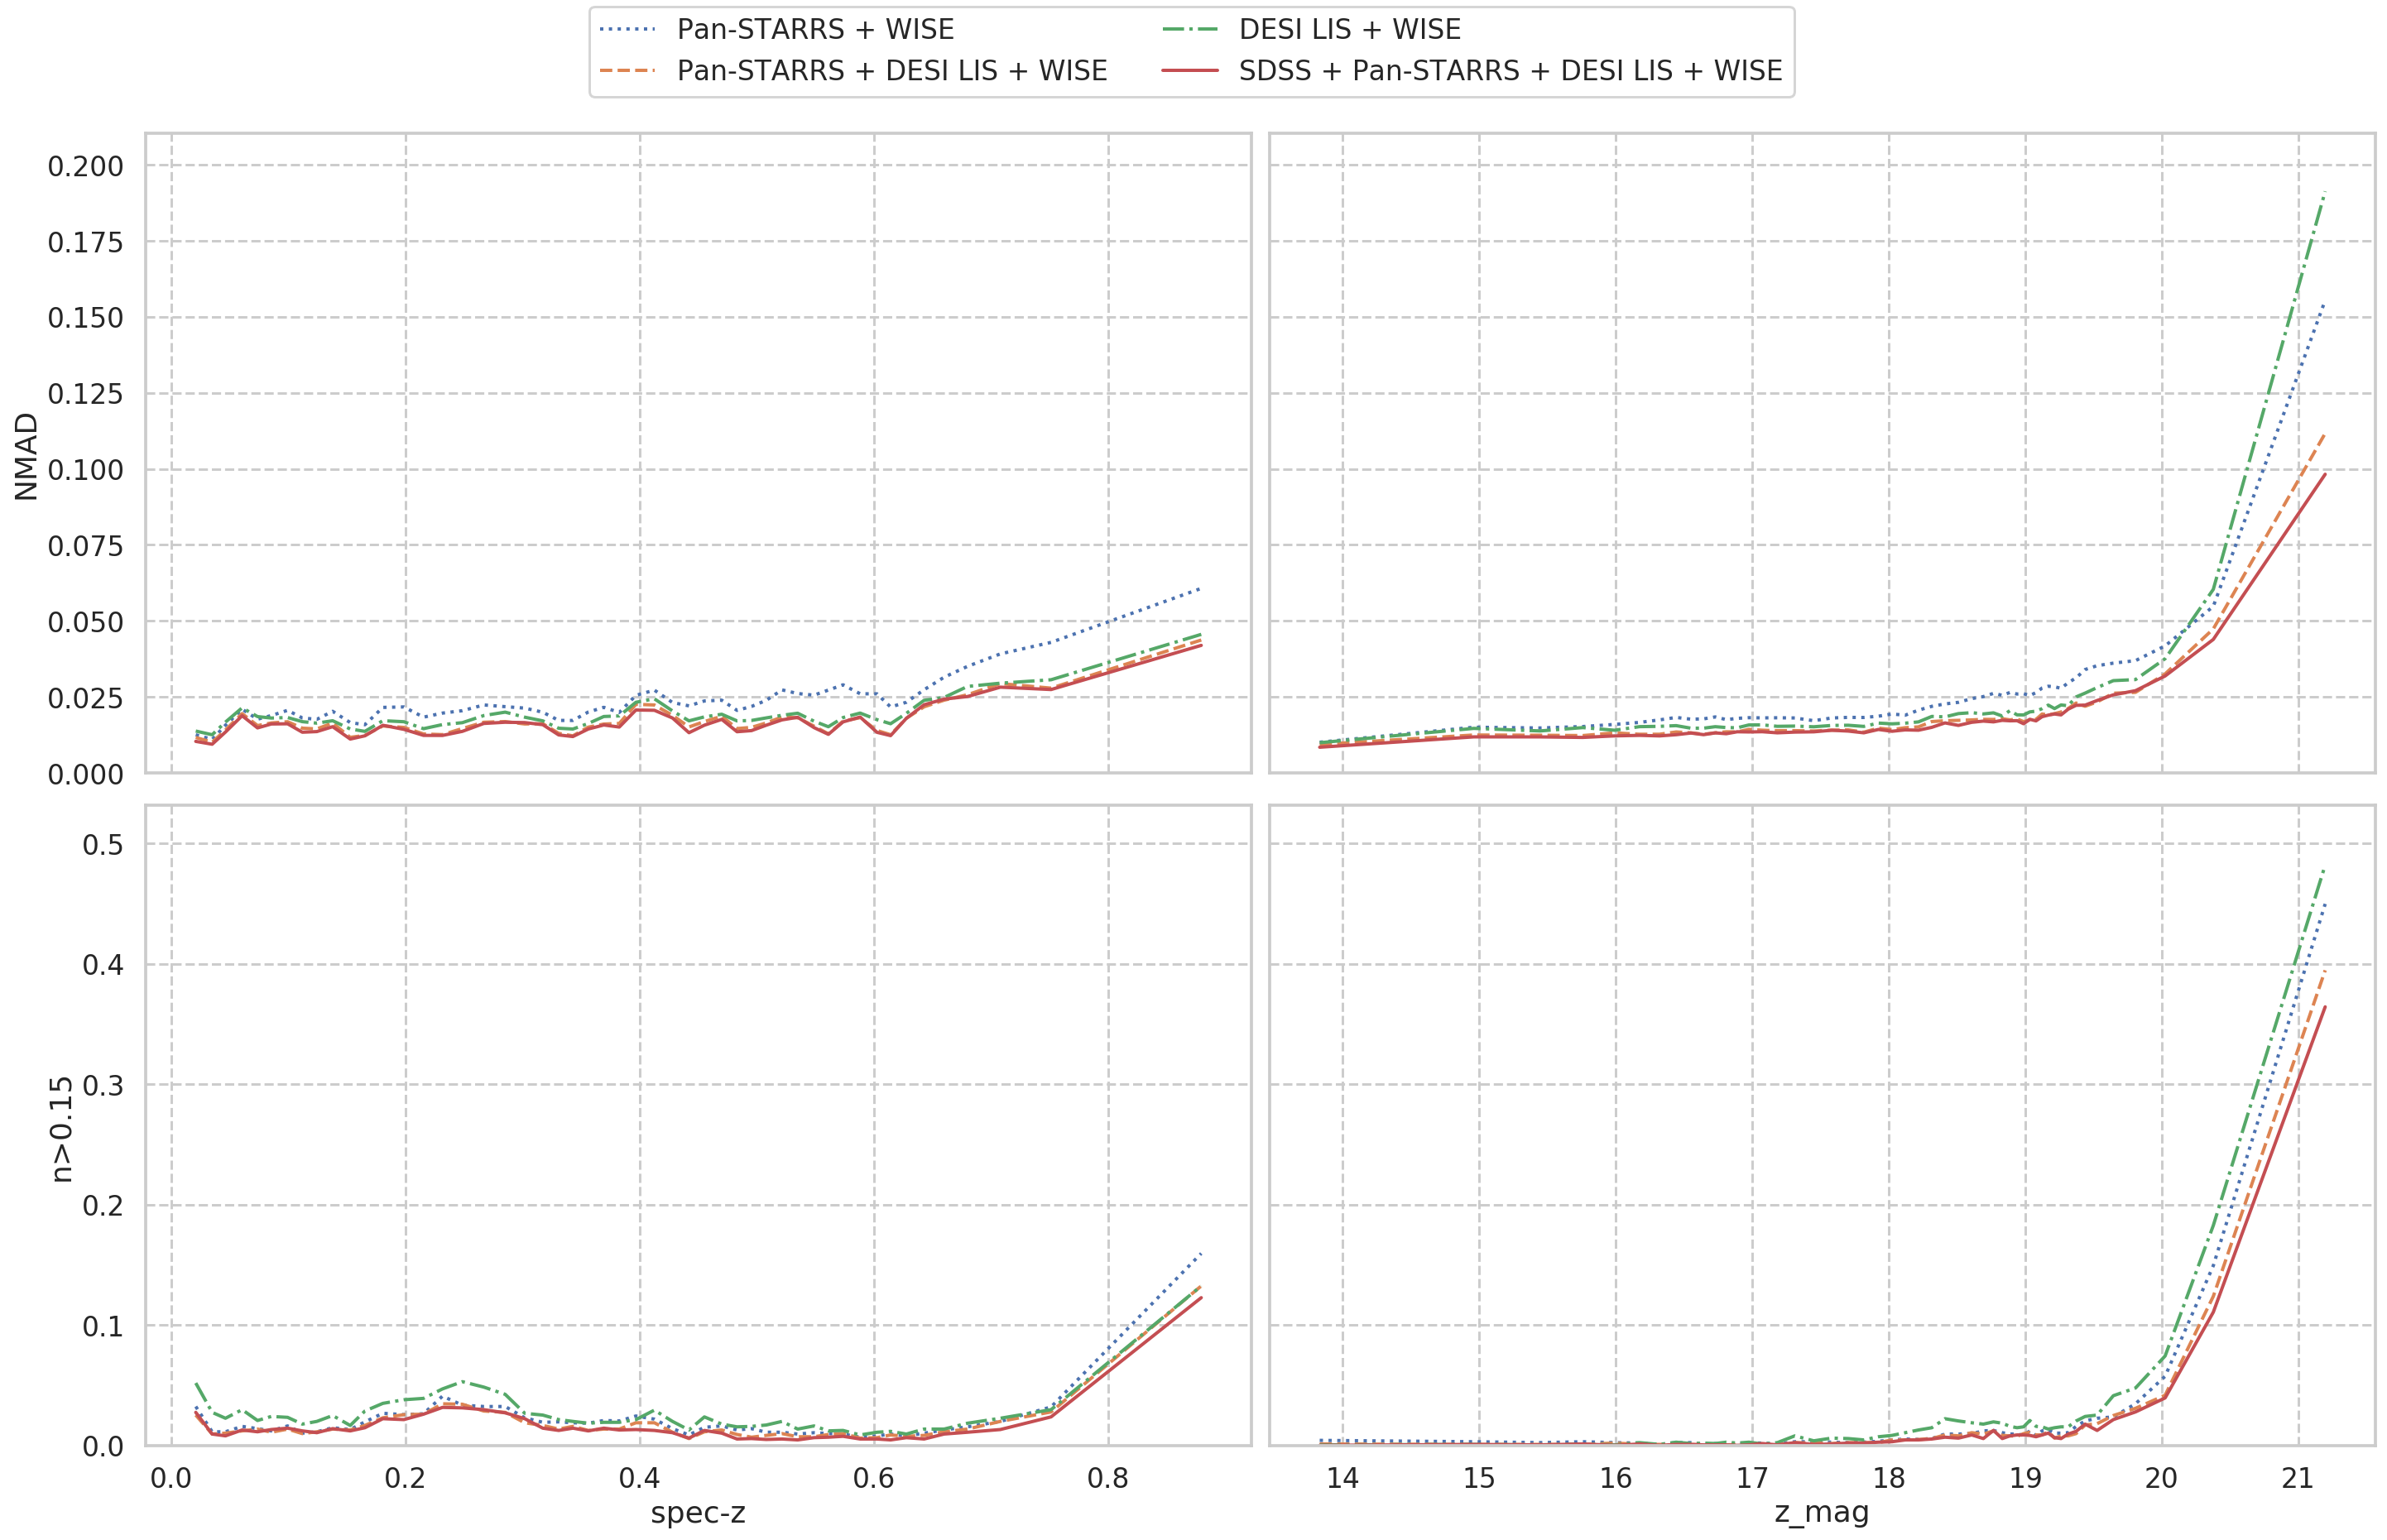
\includegraphics[width=0.9\linewidth]{images/metrics-cv2-gal.png}
%     \caption{Метрики кросс-валидации для галактик}
%     \label{fig:metrics-cv2-gal}
% \end{figure*}

\begin{figure}
    \centering
    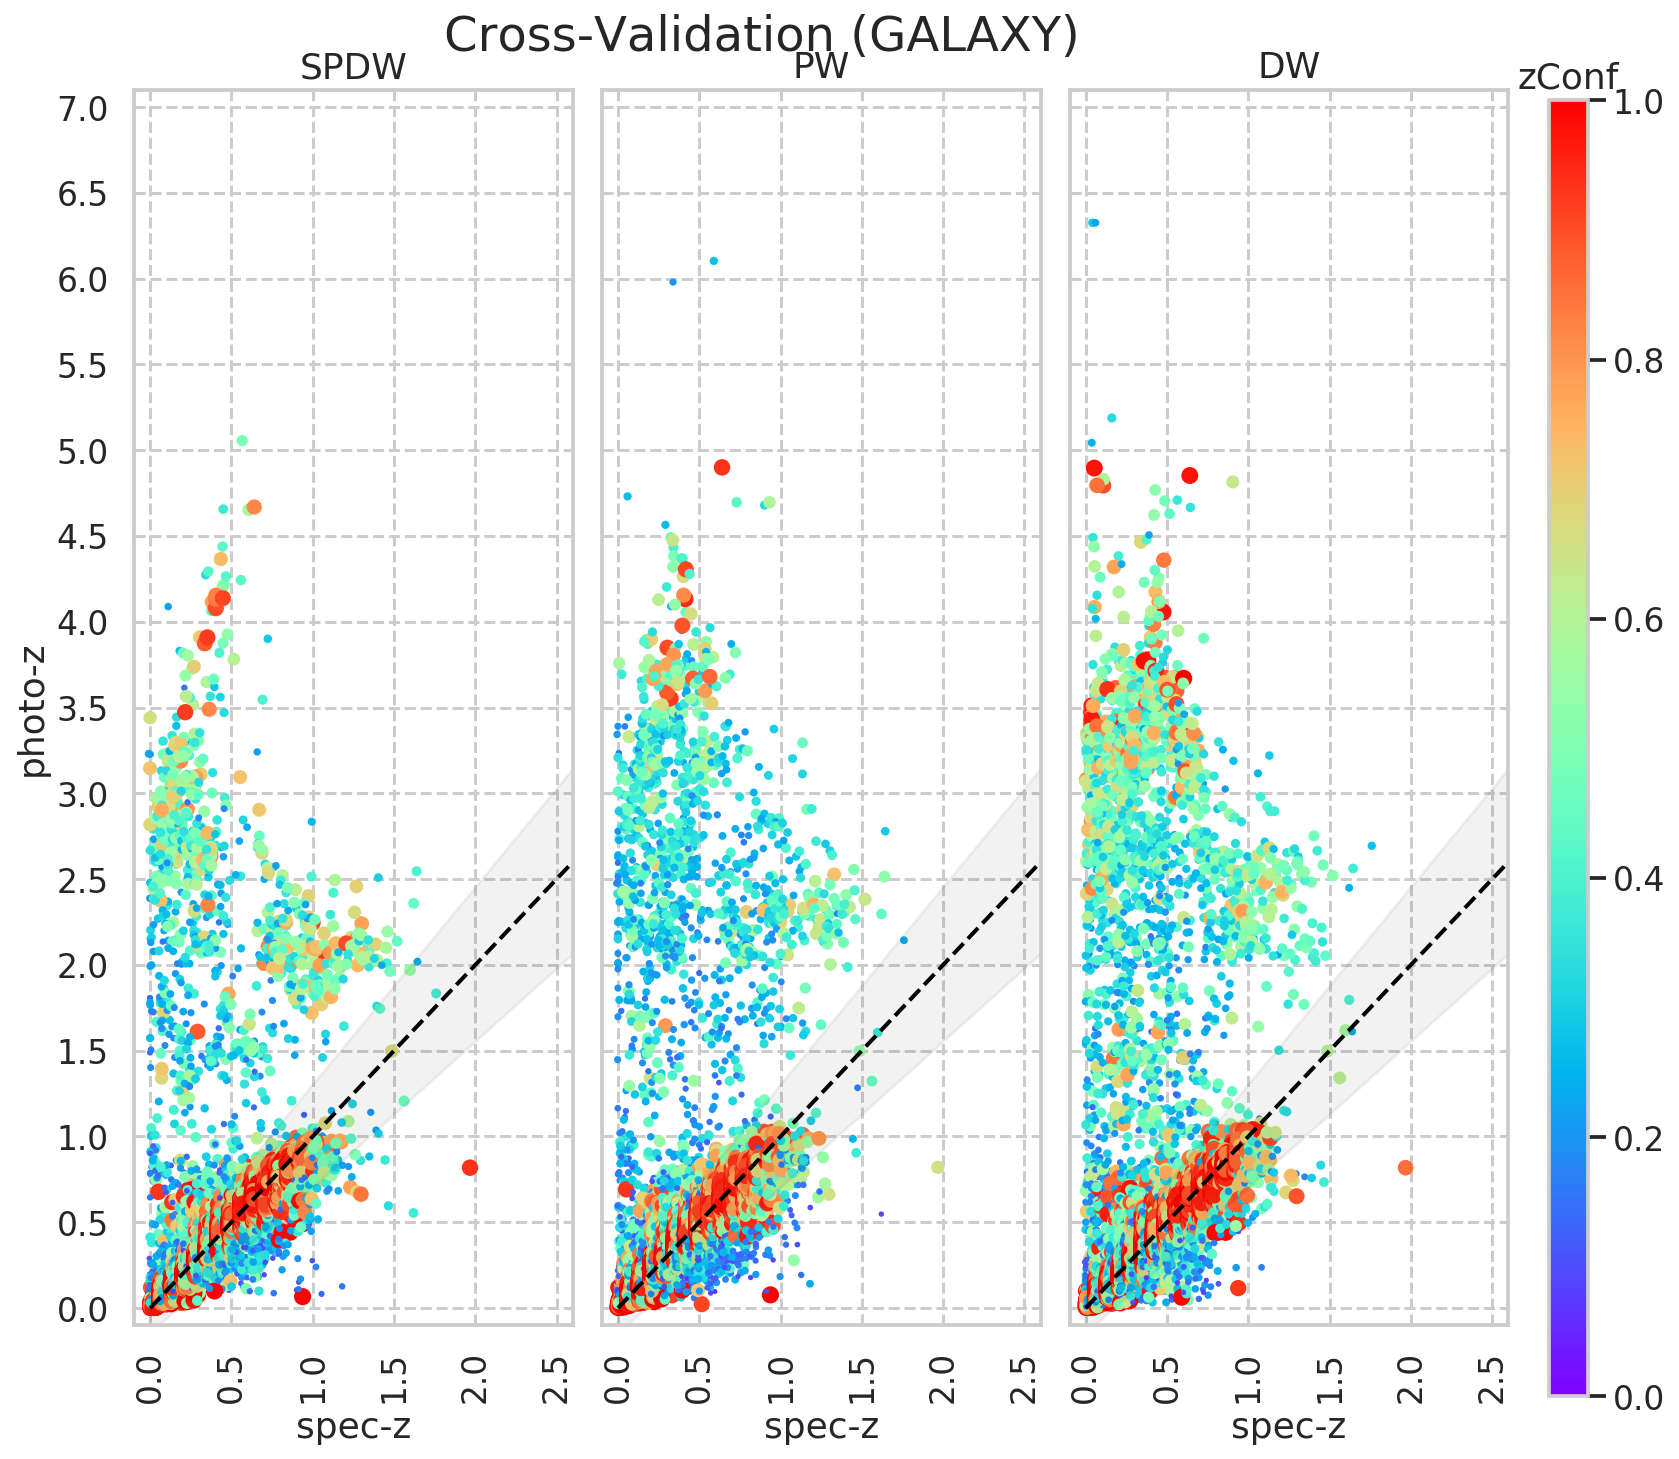
\includegraphics[width=0.9\linewidth]{images/scatterplots-cv2-gal.png}
    \caption{Скаттерплот кросс-валидации для галактик}
    \label{fig:metrics-cv2-qso}
\end{figure}

\subsection{Результаты на кросс-валидации (квазары)}
В данном разделе рассматривается поведение моделей на двукратной кросс-валидации и на тестовой выборке оптических квазаров SDSS DR16q.

Описать преимущества двукратной кросс-валидации.

Для двукратной кросс-валидации тренировочная выборка была разделена на 2 части равномерно по spec-z. Контролировать равномерность разбиения необходимо в областях с небольшим количеством обучающих примеров (например, чтобы объекты на $z > 6$ были в обеих частях в одинаковой пропорции, а не попали в одну часть).

Прогнозы двукратной кросс-валидации можно рассматривать независиомо (как? почему? зачем это надо) в том смысле, что вложения не перекрываются при обучении очередной модели, таким образом модели двукратной кросс-валидации получаются независимыми, а кросс-валидационные прогнозы можно рассматривать как прогнозы на тестовой выборке.

В результате модели показали одинаковое поведение на обоих вложениях, поэтому кросс-валидационные прогнозы будут рассмотрены вместе (криво!).

\begin{figure*}
    \centering
    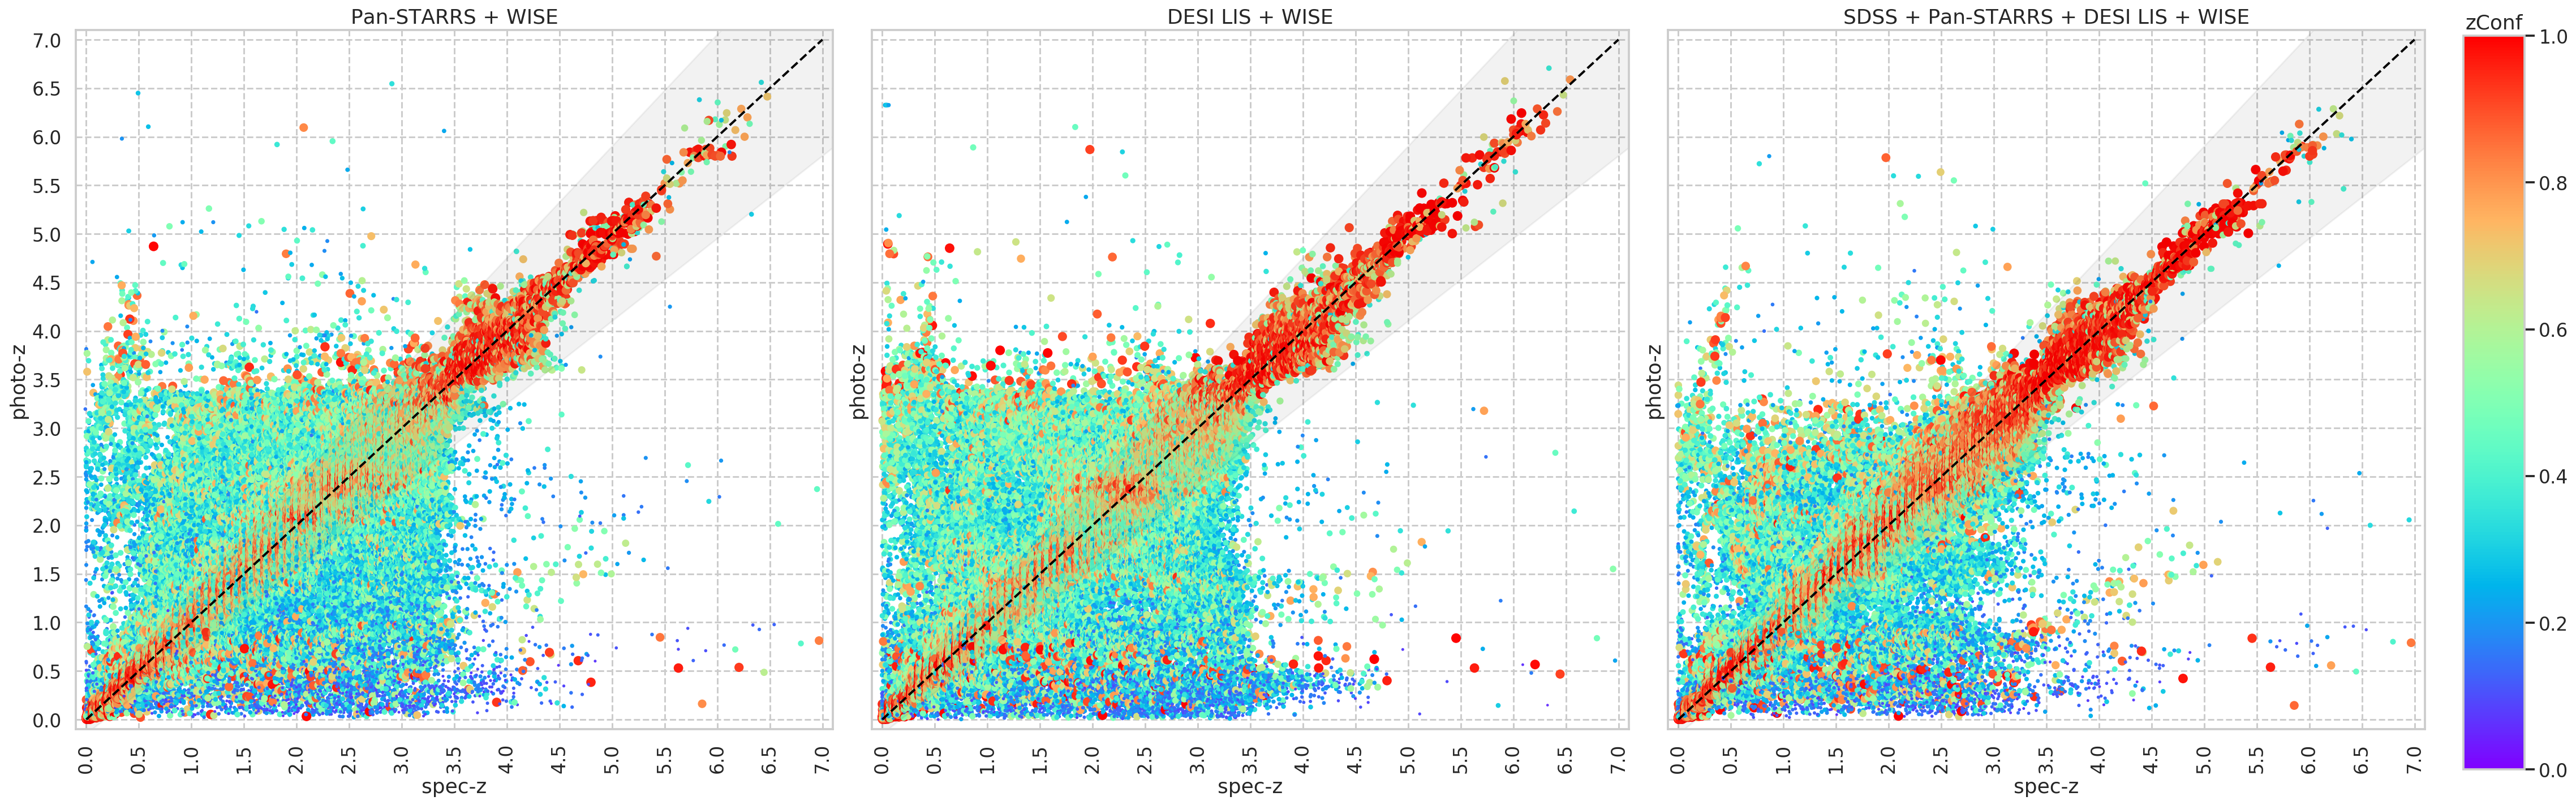
\includegraphics[width=0.9\linewidth]{images/scatterplots-cv2-total.png}
    \caption{Скаттерплот на кросс-валидации}
    \label{fig:my_label}
\end{figure*}

\begin{figure*}
    \centering
    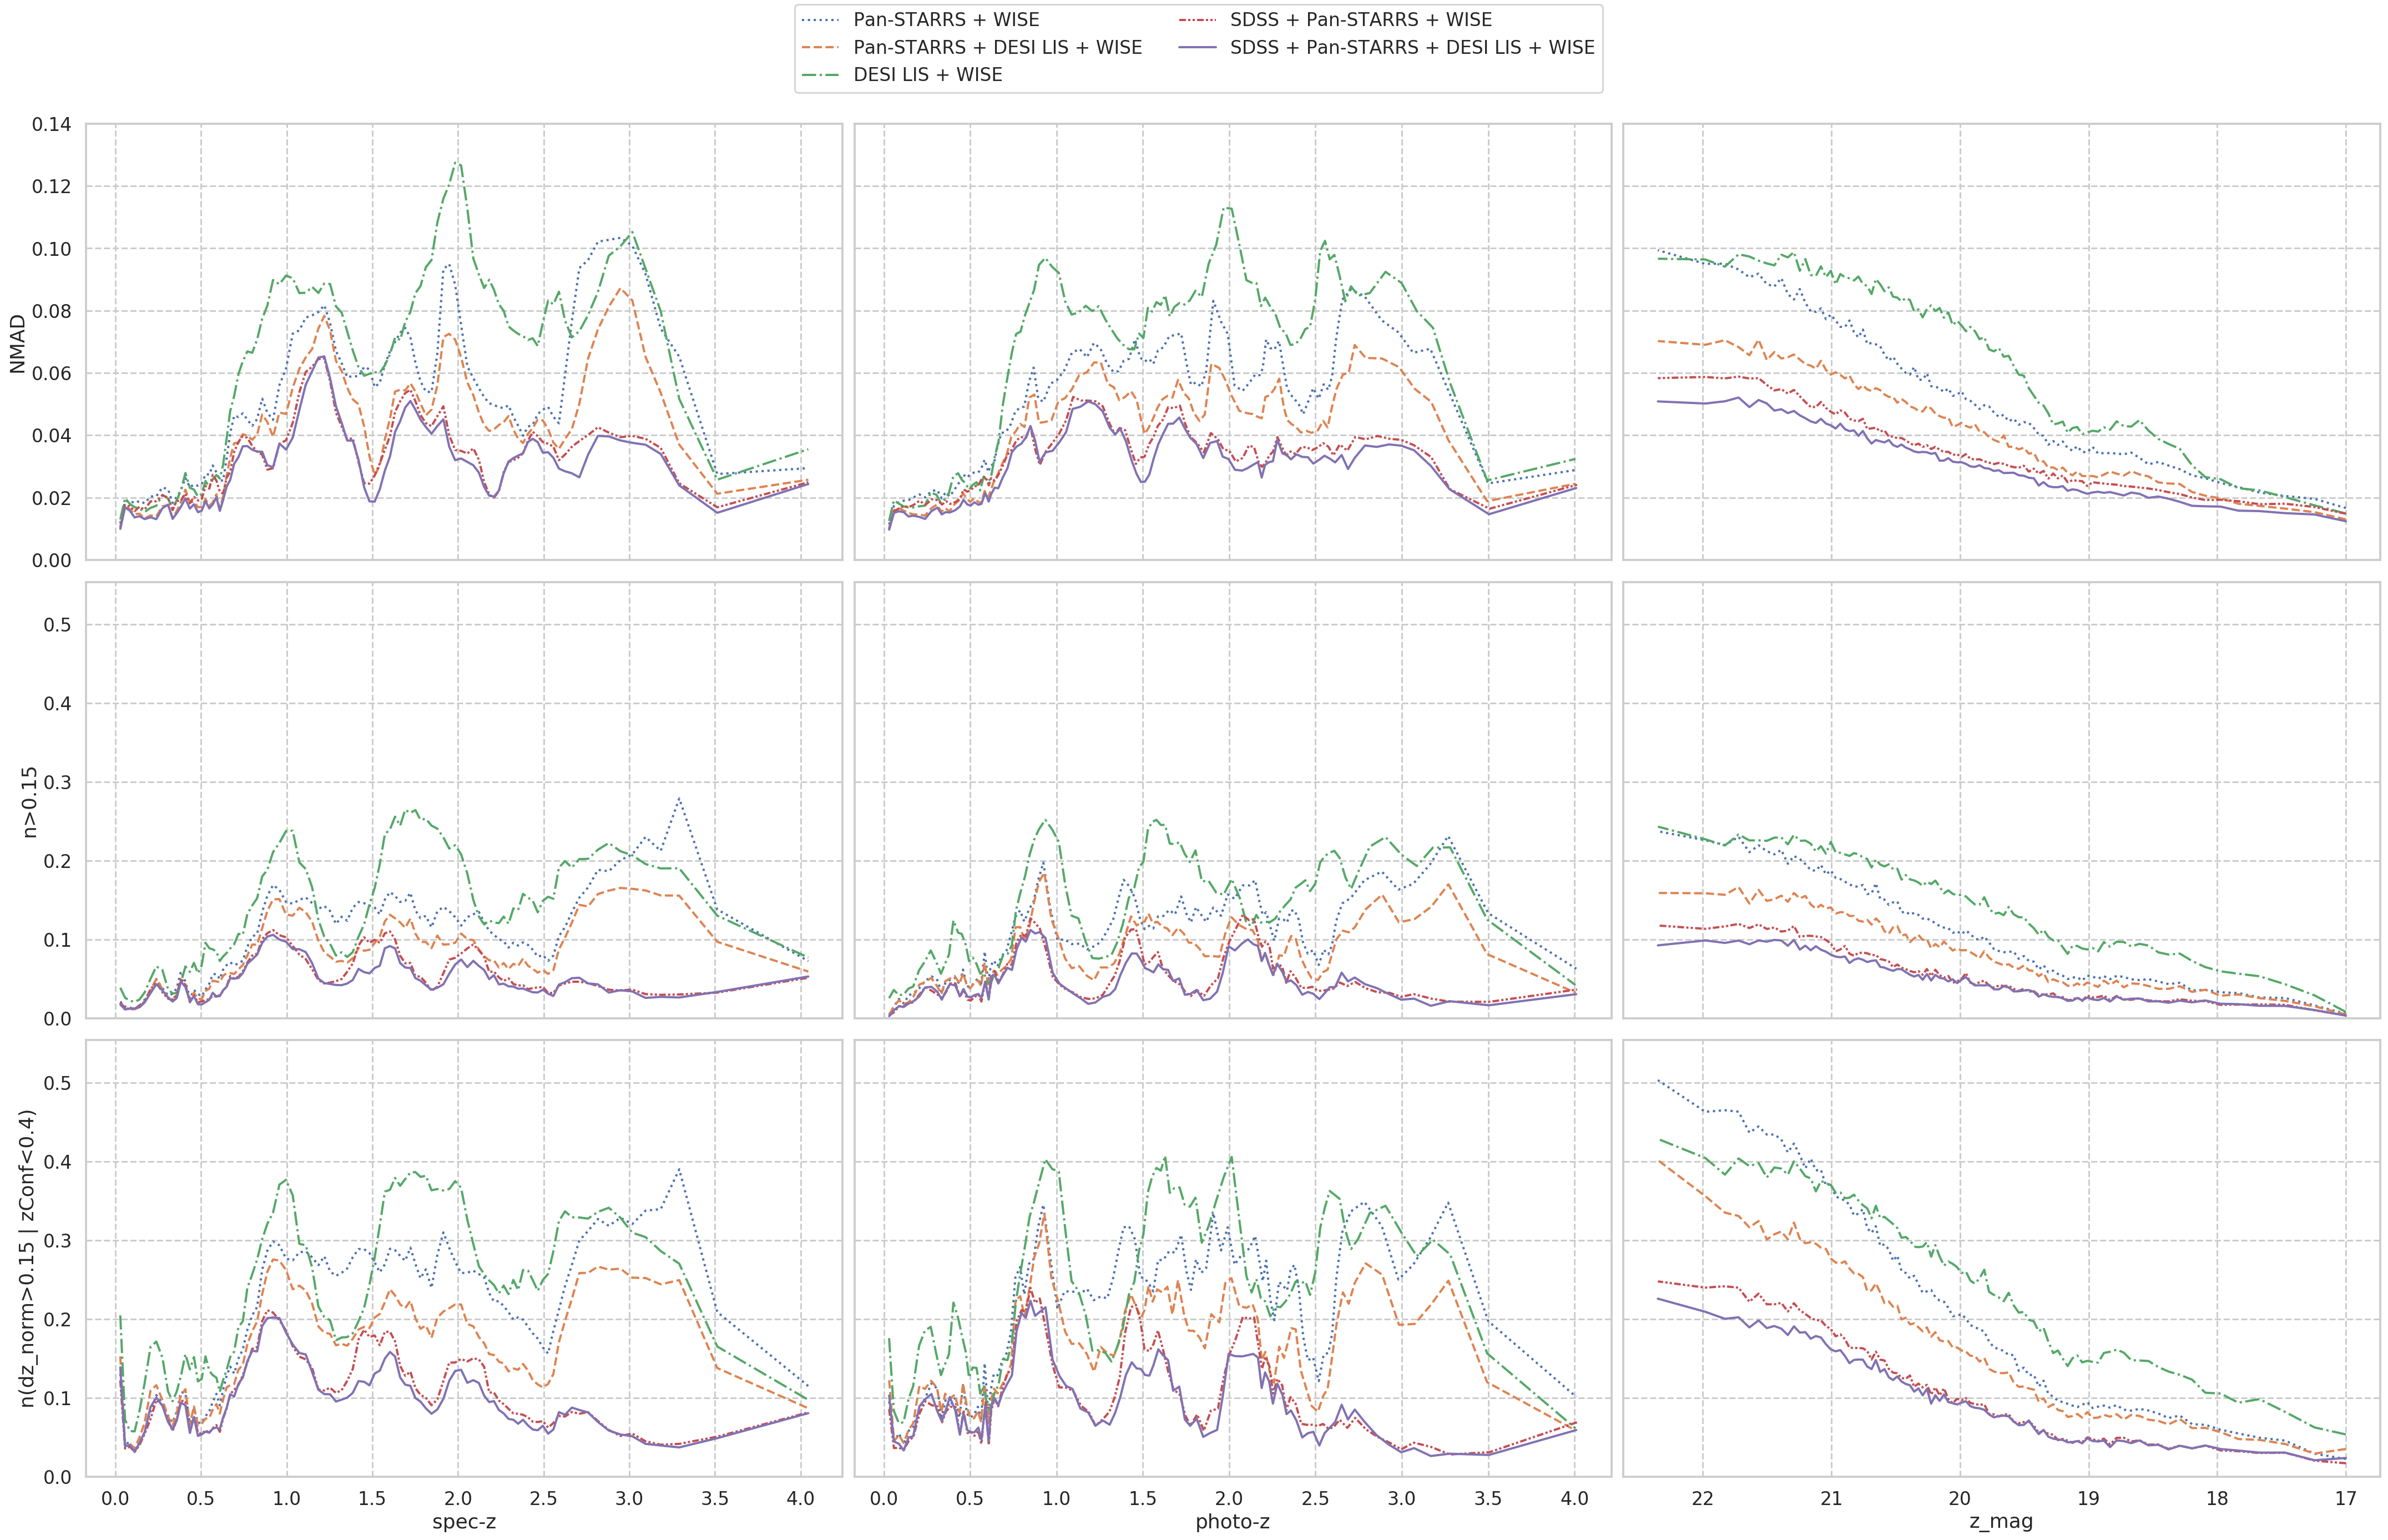
\includegraphics[width=0.9\linewidth]{images/metrics-cv2-ab.png}
    \caption{Метрики кросс-валидации}
    \label{fig:metrics-cv2-ab}
\end{figure*}

\subsection{Результаты на тестовой выборке оптических квазаров}

На рисунке \ref{fig:dr16q_wo_train} приведены диаграммы рассеяния прогнозов разных моделей на тестовой выборке оптических квазаров SDSS DR16q. Напомним, что основное различие между моделями -- используемые наборы признаков. Количество тренировочных примеров меняется незначительно (подробнее сослаться на таблицу). По диаграммам видно, что  лучше остальных на далеких объектах ($spec-z > 3,5$) себя показывают модели использующие оба каталога Pan-STARRS и DESI LIS (прогнозы лежат ближе к диагонали, меньше прогнозов с низкой достоверностью). Лучше всего в среднем ($1 < spec-z < 3$) себя показывает модель, построенная на признаках всех используемых фотометрических обзоров.

\begin{figure*}
    \centering
    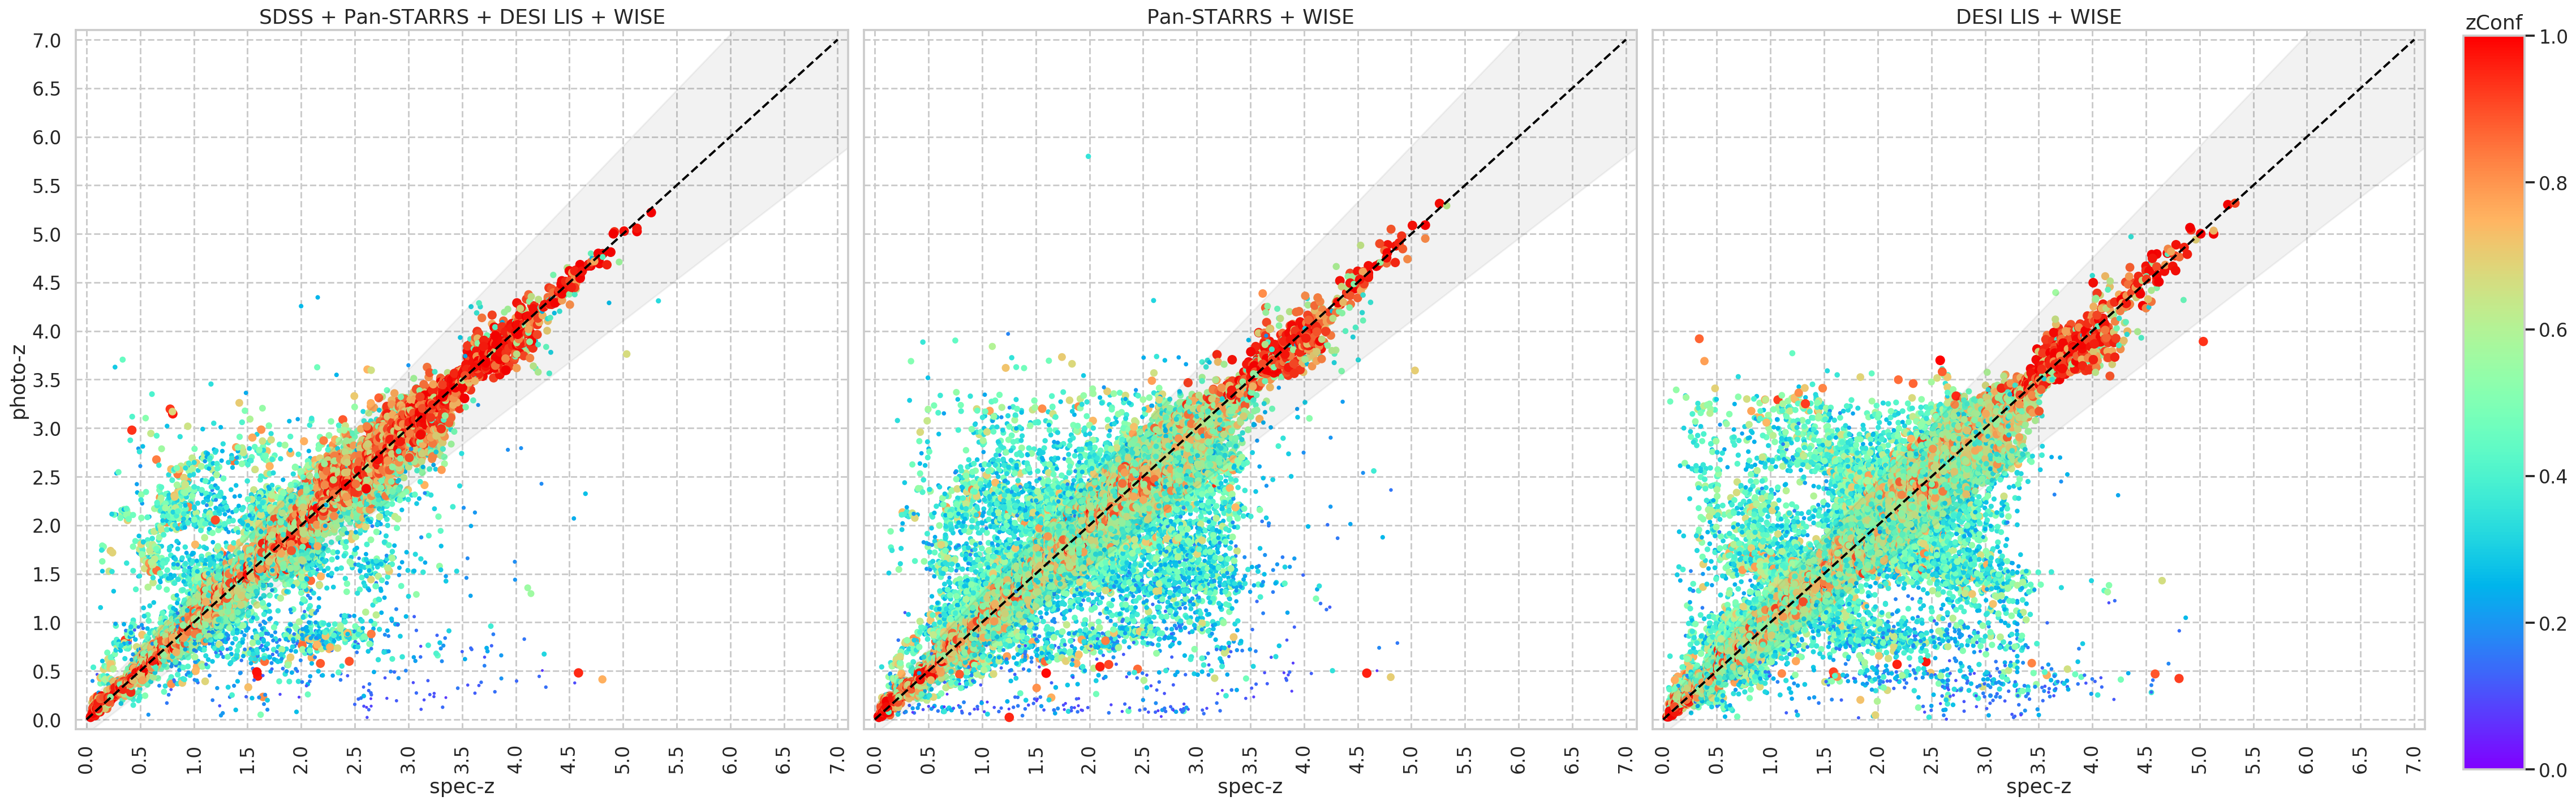
\includegraphics[width=0.9\linewidth]{images/scatterplots-dr16q-wo-train.png}
    \caption{Диаграммы рассеяния прогнозов четырех моделей Photo-z (Pan-STARRS + WISE слева сверху, Pan-STARRS + DESI LIS + WISE справа сверху, DESI LIS + WISE слева снизу и SDSS + PanSTARRS + DESI LIS + WISE справа снизу) на тестовой выборке оптических квазаров SDSS DR16q. По оси абсцисс -- значение spec-z, по оси ординат -- значение прогноза photo-z. Цветом и размером кружка показана мера достоверности прогноза zConf.}
    \label{fig:dr16q_wo_train}
\end{figure*}

\begin{figure*}
    \centering
    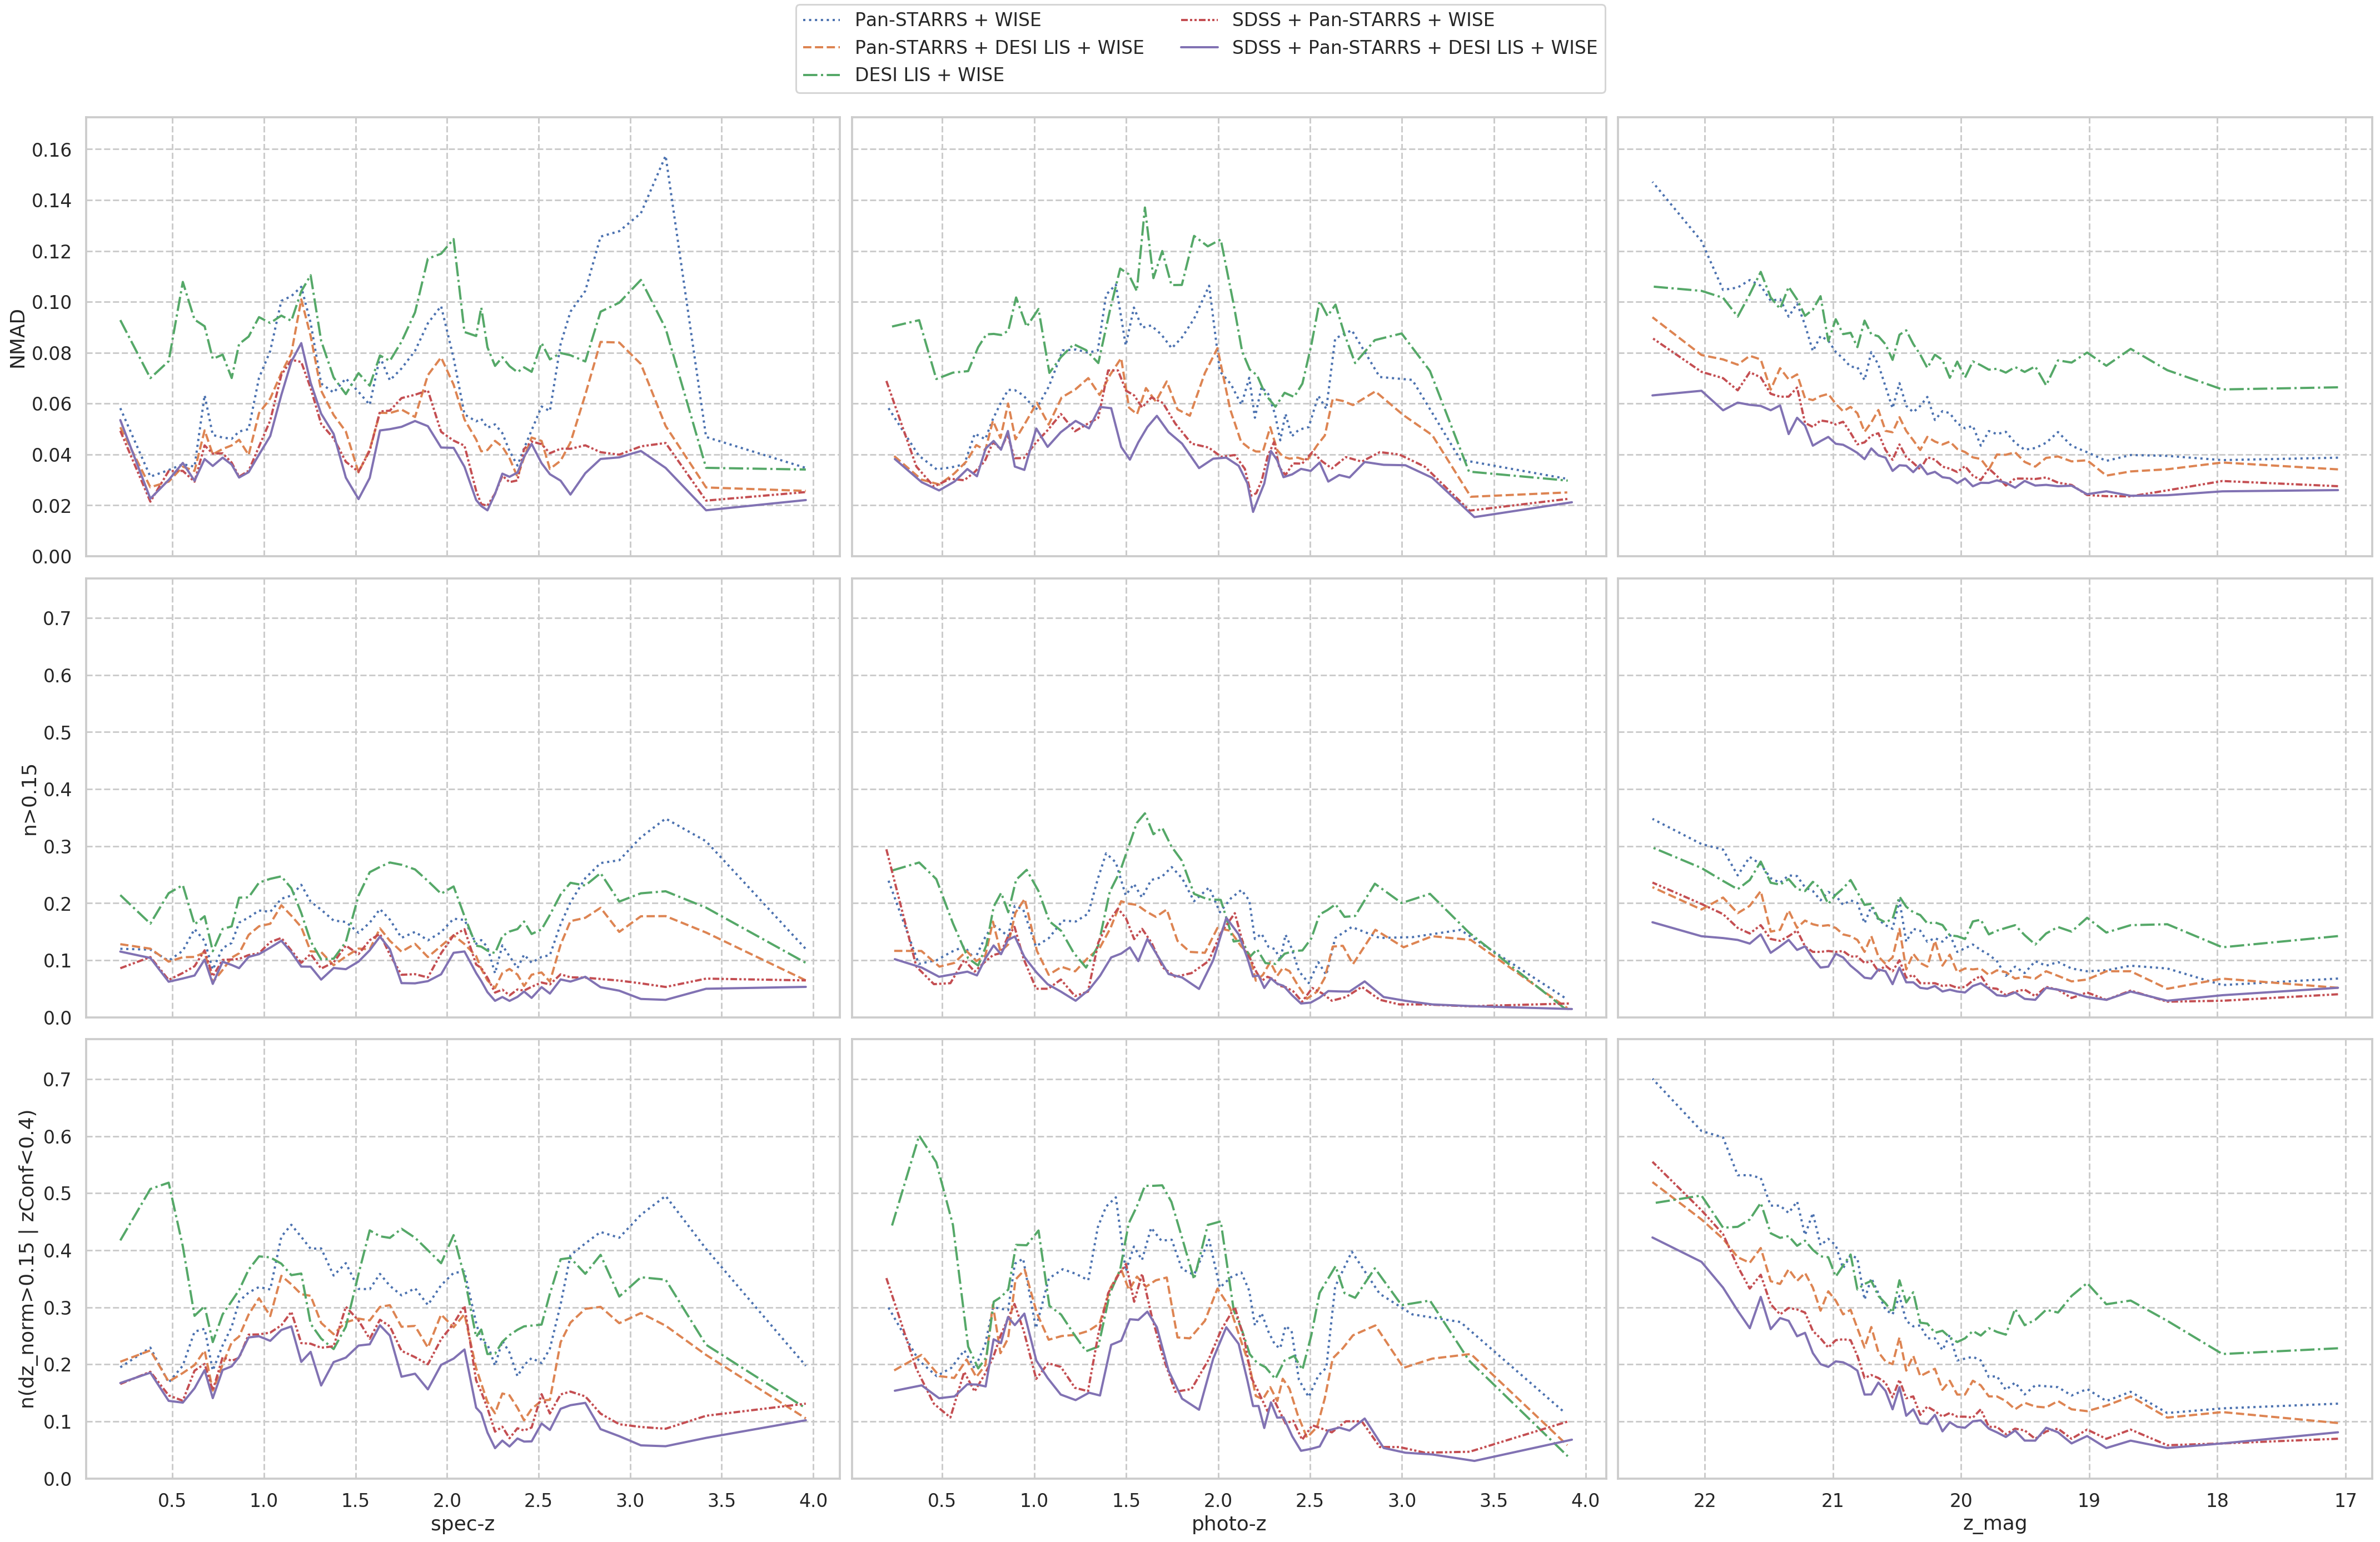
\includegraphics[width=0.9\linewidth]{images/metrics-dr16q-ab.png}
    \caption{Метрики квазаров dr16q}
    \label{fig:metrics-cv2-gal}
\end{figure*}

Это подтверждается графиками зависимости метрик от целевой переменной (спектральное красное смещение, см. рис. \ref{fig:metrics-qso_spec-z}). Из графиков так же видно, что модель DESI LIS + WISE имеет точность примерно в два раза ниже остальных моделей. Интересно, точность моделей не имеет простой (например, монотонной), зависимости от красного смещения. На разных интервалах красного смещения точность может меняться как одновременно у всех моделей, так и только у некоторых моделей. Вот некоторые наблюдения, сделанные из графиков:
% \begin{itemize}
%     \item модель DESI LIS + WISE показывает точность существенно хуже модели Pan-STARRS + WISE на $spec-z < 1$, что позволяет сделать предположение о важности фильтров $i$ и $y$ (которые присутствуют в Pan-STARRS, но отсутствуют в DESI LIS) при прогнозе для таких объектов;
%     \item то же верно для интервала $1.5 < spec-z < 2.0$;
%     \item модель SDSS + Pan-STARRS + DESI LIS + WISE показывает точность существенно выше для области $2.5 < spec-z < 3.5$, что показывает важность фильтра $u$ (который присутствует из используемых обзоров только в SDSS) для прогноза для объектов из этой области.
% \end{itemize}

% \begin{figure*}
%     \centering
%     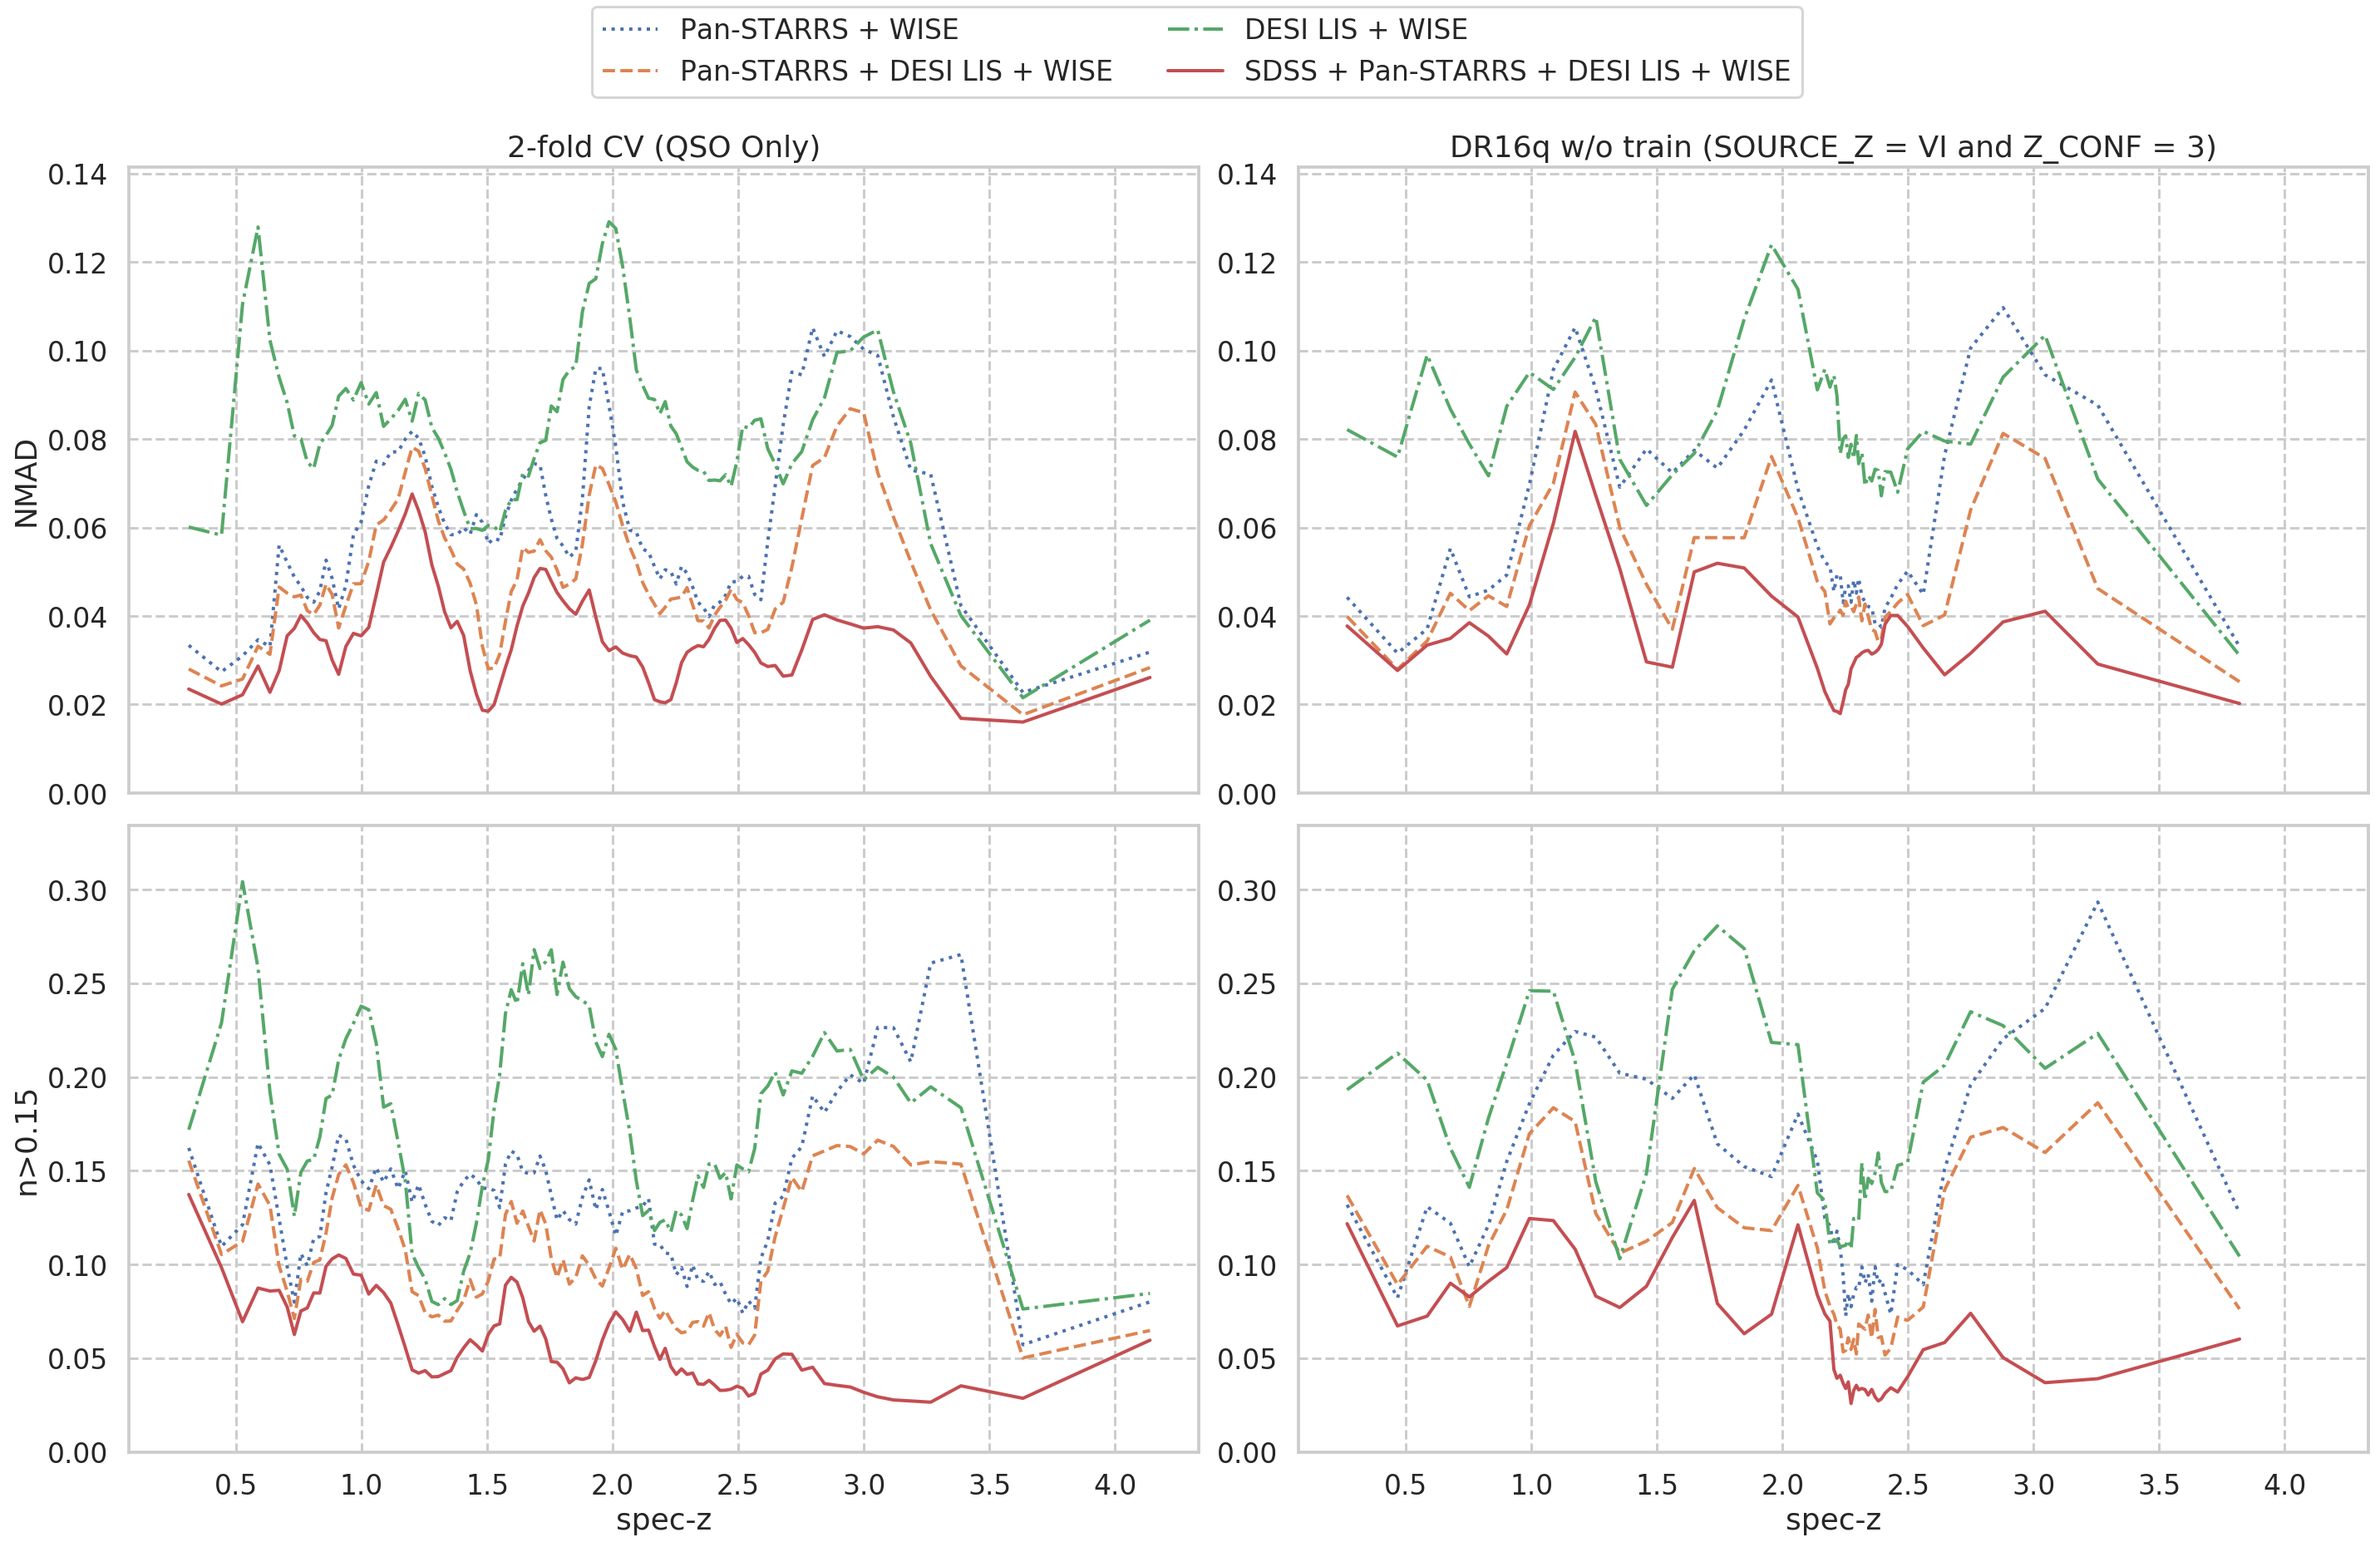
\includegraphics[width=0.9\linewidth]{images/metrics-qso_spec-z.png}
%     \caption{Графики метрик точности моделей в зависимости от значения spec-z. На верхних графиках показана метрика $NMAD$ \eqref{eq:nmad}, на нижних графиках -- доля катастрофических выбросов $n_{>0.15}$ \eqref{eq:n015}. Слева -- метрики на двукратной кросс-валидации, справа -- на тестовой выборке оптических квазаров. Модели: Pan-STARRS + WISE -- синий пунктир, DESI LIS + WISE -- зеленый штрих-пунктир, Pan-STARRS + DESI LIS + WISE -- оранжевый штрих, SDSS + DESI LIS + WISE -- красная сплошная кривая.}
%     \label{fig:metrics-qso_spec-z}
% \end{figure*}

Кроме того была обнаружена зависимость между яркостью объектов и точностью моделей. Мы приводим график только в зависимости от величины $r$ (см. рис. \ref{fig:metrics-qso_z_mag}), однако аналогичные выводы верны, если рассматривать зависимость точности от других величин. Вот некоторые выводы, которые можно сделать:
\begin{itemize}
    \item точность моделей падает на слабых объектов (например, у модели Pan-STARRS до 2.5 раз).
    \item отсутствие фильтров $i$ и $y$ приводит к понижению точности прогнозов для ярких объектов (см. модели DESI LIS + WISE и Pan-STARRS + WISE).
\end{itemize}

% \begin{figure*}
%     \centering
%     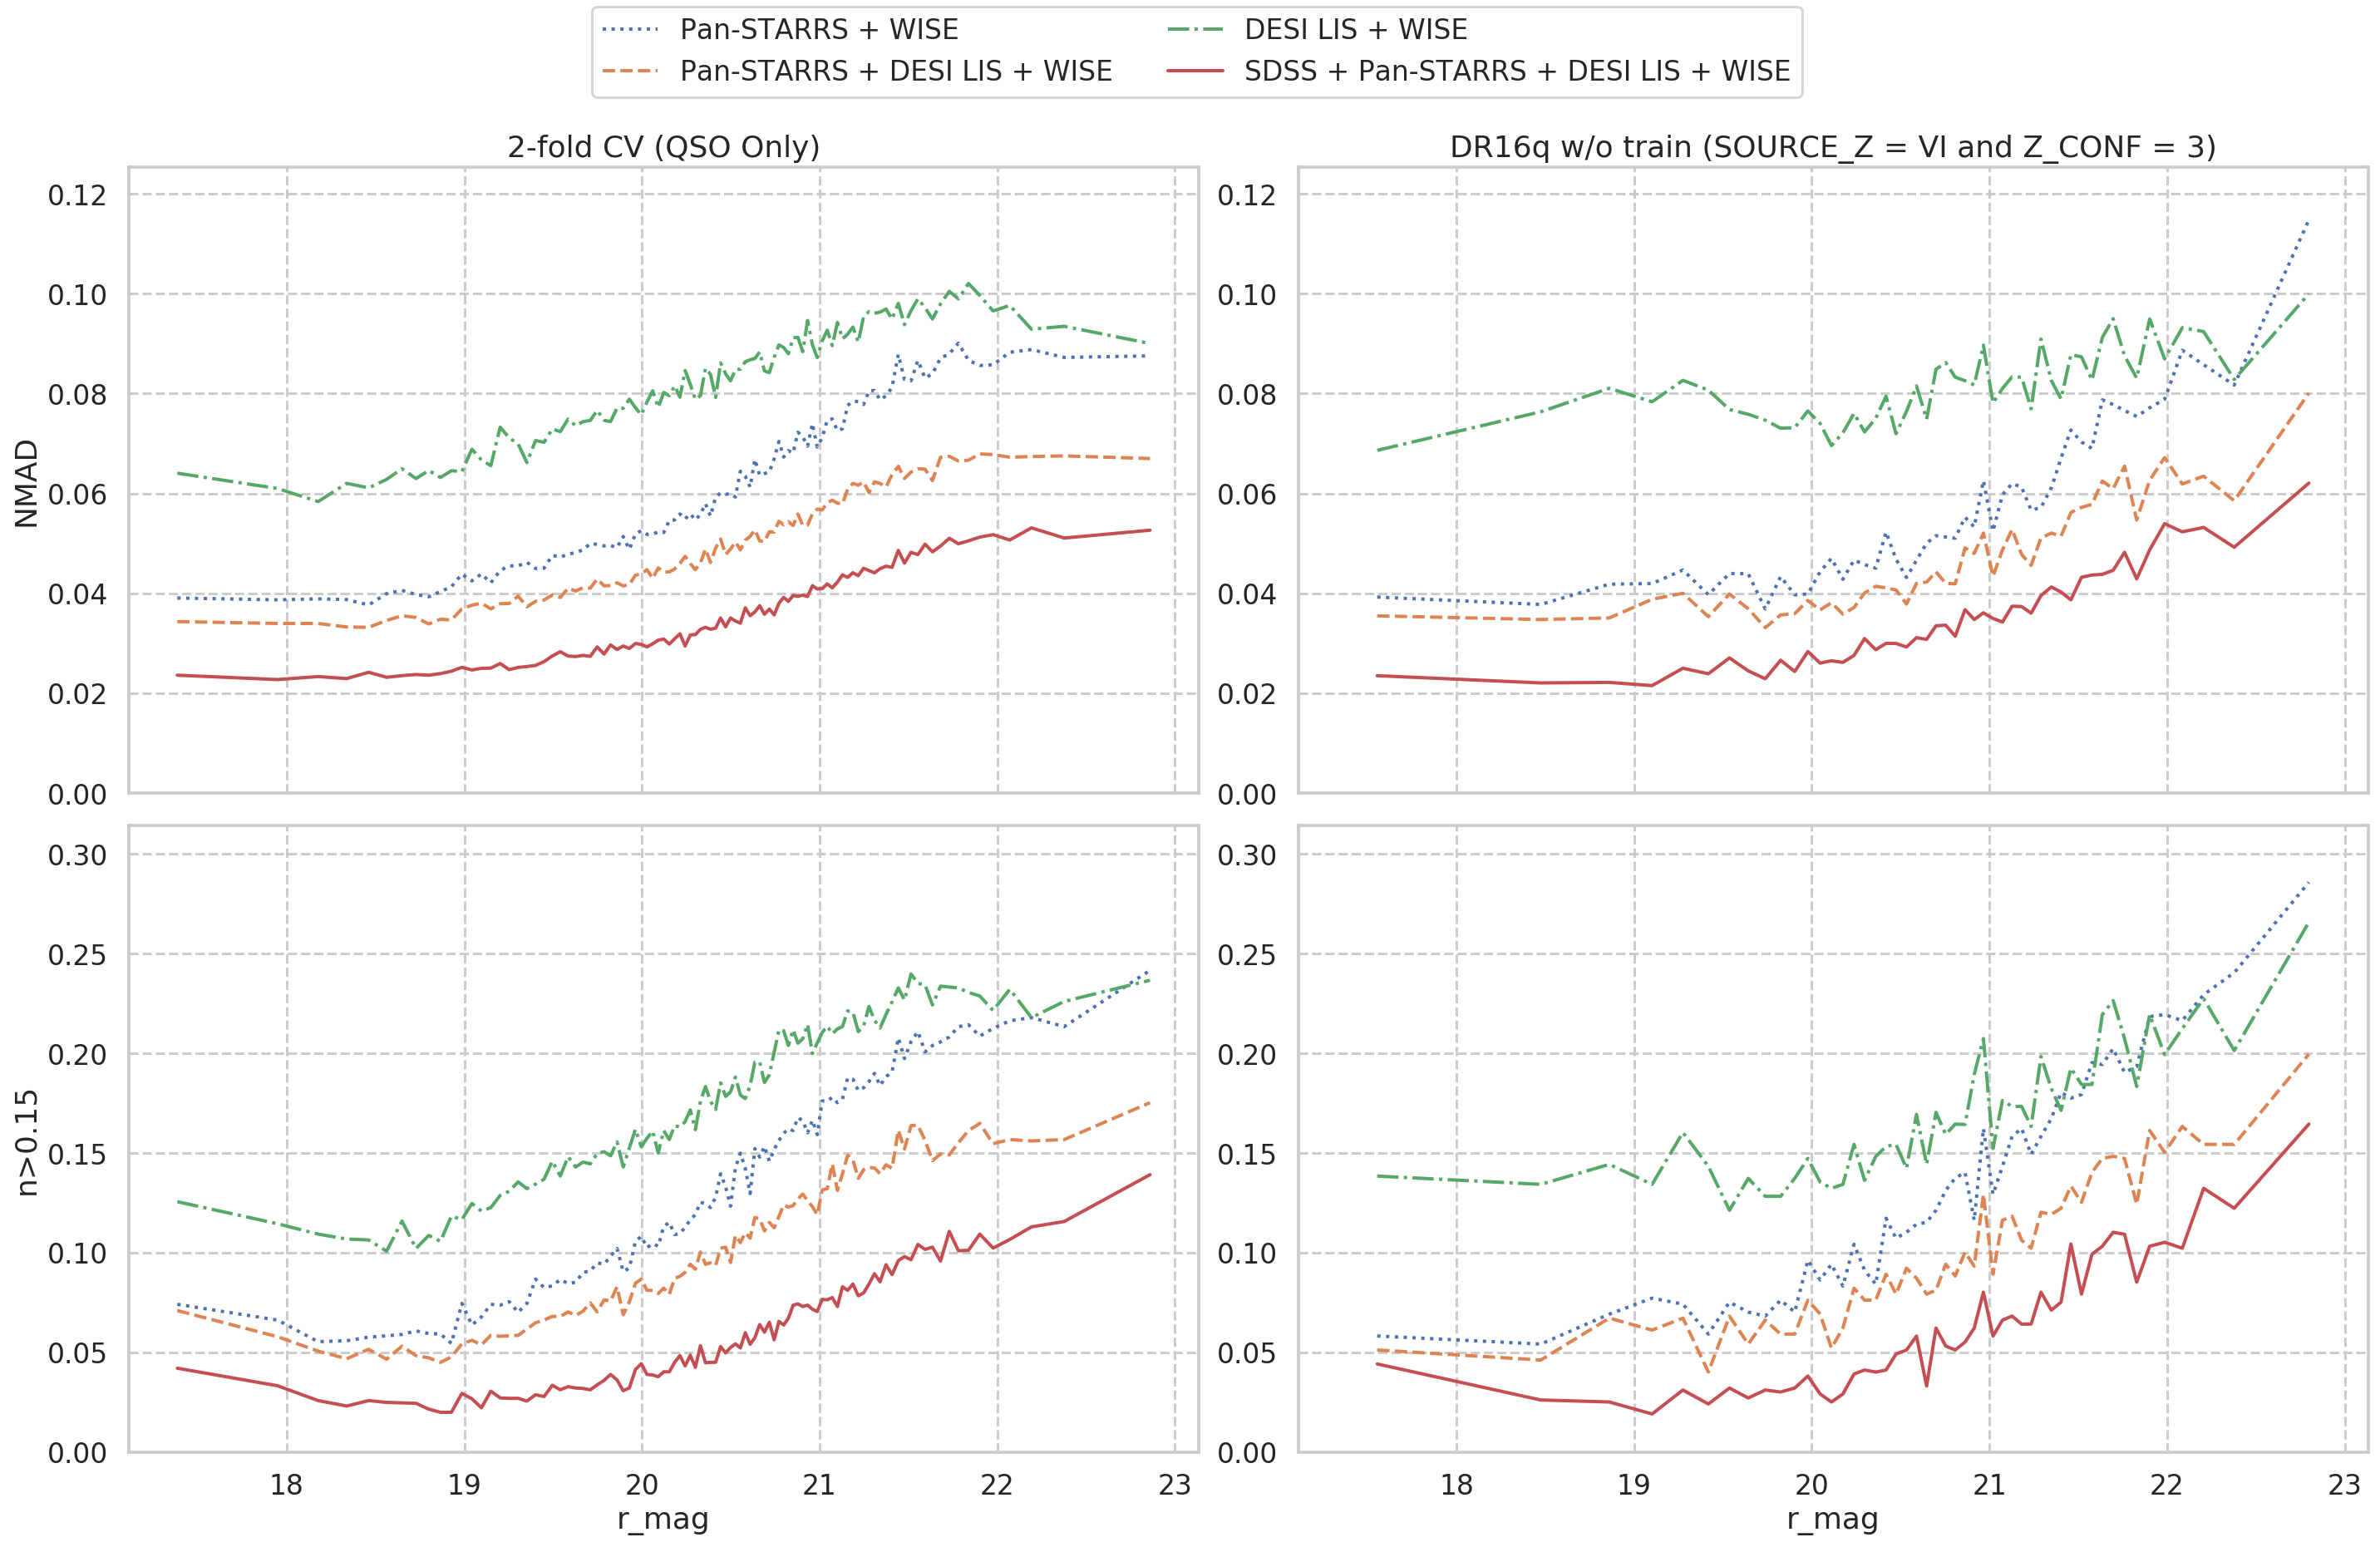
\includegraphics[width=0.9\linewidth]{images/metrics-qso_r-mag.png}
%     \caption{Графики метрик точности моделей в зависимости от значения величины $r$, посчитанной из потоков каталога DESI LIS по формуле гиперболического синуса \eqref{eq:asinhmag}. На верхних графиках показана метрика $NMAD$ \eqref{eq:nmad}, на нижних графиках -- доля катастрофических выбросов $n_{>0.15}$ \eqref{eq:n015}. Слева -- метрики на двукратной кросс-валидации, справа -- на тестовой выборке оптических квазаров. Модели: Pan-STARRS + WISE -- синий пунктир, DESI LIS + WISE -- зеленый штрих-пунктир, Pan-STARRS + DESI LIS + WISE -- оранжевый штрих, SDSS + DESI LIS + WISE -- красная сплошная кривая.}
%     \label{fig:metrics-qso_z_mag}
% \end{figure*}

\subsection{Stripe82X results}\label{subsec:s82x_results}

В данном разделе приведено описание результатов, полученных на выборке Stripe82X и сравнение с моделями (Ananna, Brescia \ref{}). В целом выводы о поведении моделей повторяют изложенное ранее в пункте \ref{}, поэтому здесь мы заострим внимание на сравнении с моделями других исследователей.

На рис. \ref{fig:s82x} показаны диаграммы рассеяния прогнозов для шести моделей. Можно видеть, что модель на основе четырех широких обзоров SDSS + Pan-STARRS + DESI LIS + WISE так же показвыает себя с лучшей стороны (прогнозы сильнее сгруппрированы вокруг диагонали, меньшая доля выбросов, точные прогнозы имеют бОльшую достоверность). Модель Ananna в свою очередь дает слишком высокую уверенность прогнозов: существенная доля катастрофических выбросов имеет $PDZbest \sim 1$.

\begin{table*}
	\begin{tabular}{llrrrrrrrrr}
            \hline
                              &                  & \multicolumn{3}{l}{Stripe82x-A17 sample} & \multicolumn{3}{l}{Quasars of DR16q} & \multicolumn{3}{l}{Cross-Validation} \\
                              &                  &               $NMAD$ &        $n>0.15$ &  $C_{68} - 0.68$ &           $NMAD$ &        $n>0.15$ &  $C_{68} - 0.68$ &           $NMAD$ &        $n>0.15$ &  $C_{68} - 0.68$ \\
            subsample & model &                      &                 &                  &                  &                 &                  &                  &                 &                  \\

\hline
            All objects       & \ref{model:pw} &                0.056 &           0.149 &            0.023 &            0.063 &           0.165 &            0.031 &            0.046 &           0.109 &            0.052 \\
                              & \ref{model:pdw} &                0.046 &           0.113 &            0.075 &            0.049 &            0.12 &            0.068 &            0.037 &           0.085 &            0.072 \\
                              & \ref{model:dw} &                0.074 &           0.177 &  \textbf{-0.003} &            0.083 &            0.19 &  \textbf{-0.005} &            0.058 &           0.143 &  \textbf{-0.008} \\
                              & \ref{model:spw} &                 0.04 &           0.105 &            0.089 &             0.04 &           0.088 &            0.082 &            0.031 &           0.054 &            0.084 \\
                              & \ref{model:spdw} &       \textbf{0.034} &  \textbf{0.089} &            0.104 &   \textbf{0.037} &  \textbf{0.076} &            0.093 &   \textbf{0.028} &  \textbf{0.048} &            0.093 \\
\hline
\hline
            $z_{spec} < 0.5$ & \ref{model:pw} &                0.038 &  \textbf{0.083} &   \textbf{0.003} &            0.038 &           0.113 &   \textbf{0.028} &             0.02 &           0.031 &            0.045 \\
                              & \ref{model:pdw} &                0.031 &           0.086 &             0.04 &            0.033 &           0.112 &            0.044 &            0.016 &           0.027 &            0.072 \\
                              & \ref{model:dw} &                0.048 &           0.111 &            0.035 &            0.077 &           0.197 &           -0.056 &            0.019 &           0.045 &  \textbf{-0.004} \\
                              & \ref{model:spw} &                0.032 &  \textbf{0.083} &            0.044 &            0.032 &  \textbf{0.085} &            0.063 &            0.018 &           0.026 &            0.076 \\
                              & \ref{model:spdw} &        \textbf{0.03} &           0.084 &            0.062 &   \textbf{0.031} &           0.097 &            0.056 &   \textbf{0.015} &  \textbf{0.025} &            0.094 \\
\hline
            $0.5 \leq z_{spec} < 1$ & \ref{model:pw} &                0.053 &           0.147 &             0.03 &            0.048 &           0.139 &            0.061 &            0.037 &           0.088 &             0.06 \\
                              & \ref{model:pdw} &                0.047 &           0.138 &            0.072 &            0.042 &           0.112 &            0.084 &             0.03 &           0.078 &             0.08 \\
                              & \ref{model:dw} &                0.081 &           0.204 &  \textbf{-0.011} &            0.085 &           0.186 &  \textbf{-0.023} &            0.049 &           0.126 &  \textbf{-0.013} \\
                              & \ref{model:spw} &                0.043 &           0.111 &            0.109 &            0.037 &           0.097 &            0.106 &             0.03 &            0.06 &            0.099 \\
                              & \ref{model:spdw} &       \textbf{0.038} &  \textbf{0.106} &            0.122 &   \textbf{0.035} &  \textbf{0.089} &            0.124 &   \textbf{0.026} &  \textbf{0.058} &            0.111 \\
\hline
            $1 \leq z_{spec} < 1.5$ & \ref{model:pw} &                0.079 &           0.173 &            0.025 &            0.083 &           0.195 &            0.031 &            0.069 &           0.142 &            0.051 \\
                              & \ref{model:pdw} &                0.061 &           0.109 &            0.074 &             0.07 &           0.146 &            0.066 &            0.059 &           0.099 &            0.074 \\
                              & \ref{model:dw} &                0.083 &           0.143 &    \textbf{0.01} &            0.088 &           0.177 &   \textbf{0.005} &            0.078 &           0.134 &   \textbf{0.019} \\
                              & \ref{model:spw} &                0.053 &           0.108 &            0.097 &            0.058 &           0.113 &             0.11 &            0.046 &            0.07 &            0.099 \\
                              & \ref{model:spdw} &       \textbf{0.048} &  \textbf{0.088} &            0.122 &   \textbf{0.057} &    \textbf{0.1} &            0.107 &   \textbf{0.043} &   \textbf{0.06} &            0.105 \\
\hline
            $1.5 \leq z_{spec} < 2$ & \ref{model:pw} &                0.075 &           0.158 &            0.075 &            0.076 &           0.157 &            0.088 &            0.069 &           0.142 &            0.061 \\
                              & \ref{model:pdw} &                0.043 &           0.102 &            0.127 &            0.056 &           0.128 &            0.088 &            0.051 &           0.109 &            0.077 \\
                              & \ref{model:dw} &                0.078 &           0.253 &  \textbf{-0.029} &            0.093 &           0.256 &  \textbf{-0.009} &            0.089 &           0.238 &  \textbf{-0.042} \\
                              & \ref{model:spw} &                 0.04 &           0.096 &            0.163 &            0.053 &           0.103 &            0.115 &            0.043 &           0.073 &            0.101 \\
                              & \ref{model:spdw} &       \textbf{0.031} &  \textbf{0.065} &            0.144 &   \textbf{0.044} &  \textbf{0.093} &             0.12 &   \textbf{0.038} &  \textbf{0.061} &            0.105 \\
\hline
            $2 \leq z_{spec}$ & \ref{model:pw} &                0.071 &           0.222 &  \textbf{-0.018} &            0.063 &           0.173 &  \textbf{-0.001} &            0.058 &           0.132 &            0.046 \\
                              & \ref{model:pdw} &                0.046 &           0.133 &            0.089 &            0.046 &           0.111 &            0.059 &            0.047 &           0.101 &            0.064 \\
                              & \ref{model:dw} &                0.091 &           0.206 &           -0.043 &            0.078 &           0.172 &            0.005 &             0.08 &           0.164 &  \textbf{-0.002} \\
                              & \ref{model:spw} &                0.039 &            0.14 &             0.03 &            0.035 &            0.07 &            0.053 &            0.033 &           0.048 &            0.064 \\
                              & \ref{model:spdw} &       \textbf{0.029} &  \textbf{0.098} &            0.072 &   \textbf{0.031} &  \textbf{0.055} &            0.072 &    \textbf{0.03} &  \textbf{0.043} &            0.072 \\
\hline
\hline
            $z_{mag} < 19$ & \ref{model:pw} &                0.037 &           0.046 &   \textbf{0.015} &            0.039 &           0.077 &            0.053 &            0.025 &           0.033 &            0.059 \\
                                   & \ref{model:pdw} &                0.027 &            0.04 &            0.043 &            0.034 &           0.068 &            0.066 &             0.02 &           0.029 &            0.077 \\
                                   & \ref{model:dw} &                0.038 &            0.08 &            0.036 &            0.071 &           0.152 &  \textbf{-0.012} &            0.026 &            0.06 &  \textbf{-0.006} \\
                                   & \ref{model:spw} &       \textbf{0.024} &           0.038 &            0.062 &            0.026 &  \textbf{0.035} &            0.102 &            0.019 &           0.018 &            0.092 \\
                                   & \ref{model:spdw} &       \textbf{0.024} &  \textbf{0.029} &            0.081 &   \textbf{0.025} &            0.04 &            0.096 &   \textbf{0.017} &  \textbf{0.017} &            0.104 \\
\hline
            $19 \leq z_{mag} < 20$ & \ref{model:pw} &                0.043 &           0.076 &            0.075 &            0.046 &           0.098 &            0.065 &            0.043 &           0.079 &            0.059 \\
                                   & \ref{model:pdw} &                0.036 &           0.065 &            0.114 &            0.038 &           0.075 &            0.082 &            0.035 &           0.064 &            0.076 \\
                                   & \ref{model:dw} &                0.071 &            0.11 &   \textbf{0.008} &            0.074 &           0.154 &  \textbf{-0.004} &            0.058 &           0.124 &  \textbf{-0.006} \\
                                   & \ref{model:spw} &                0.031 &           0.045 &            0.115 &             0.03 &            0.05 &            0.095 &            0.029 &           0.037 &             0.09 \\
                                   & \ref{model:spdw} &       \textbf{0.028} &  \textbf{0.041} &            0.131 &   \textbf{0.028} &  \textbf{0.044} &            0.099 &   \textbf{0.027} &  \textbf{0.035} &            0.097 \\
\hline
            $20 \leq z_{mag} < 20.5$ & \ref{model:pw} &                0.064 &           0.137 &            0.027 &            0.058 &           0.145 &            0.031 &            0.058 &           0.129 &            0.052 \\
                                   & \ref{model:pdw} &                0.046 &           0.105 &            0.107 &            0.045 &           0.105 &            0.069 &            0.048 &             0.1 &            0.071 \\
                                   & \ref{model:dw} &                0.075 &           0.165 &   \textbf{0.014} &            0.079 &           0.172 &   \textbf{0.007} &            0.081 &           0.174 &  \textbf{-0.007} \\
                                   & \ref{model:spw} &                0.041 &           0.087 &            0.105 &            0.037 &           0.065 &            0.083 &            0.037 &           0.059 &            0.087 \\
                                   & \ref{model:spdw} &       \textbf{0.033} &  \textbf{0.074} &            0.107 &   \textbf{0.033} &  \textbf{0.056} &            0.101 &   \textbf{0.034} &  \textbf{0.054} &            0.094 \\
\hline
            $20.5 \leq z_{mag} < 21$ & \ref{model:pw} &                0.076 &           0.199 &           -0.009 &            0.072 &           0.183 &            0.024 &            0.072 &           0.168 &             0.04 \\
                                   & \ref{model:pdw} &                0.056 &           0.121 &            0.078 &            0.054 &           0.127 &            0.077 &            0.057 &           0.128 &            0.063 \\
                                   & \ref{model:dw} &                0.088 &           0.219 &   \textbf{0.006} &            0.084 &           0.198 &   \textbf{0.004} &            0.089 &           0.206 &  \textbf{-0.011} \\
                                   & \ref{model:spw} &                0.054 &           0.126 &            0.076 &            0.046 &           0.099 &            0.067 &            0.044 &           0.083 &            0.072 \\
                                   & \ref{model:spdw} &       \textbf{0.044} &  \textbf{0.106} &            0.105 &   \textbf{0.039} &  \textbf{0.082} &             0.09 &    \textbf{0.04} &  \textbf{0.073} &            0.081 \\
\hline
            $21 \leq z_{mag} < 23$ & \ref{model:pw} &                0.119 &           0.319 &  \textbf{-0.011} &            0.102 &           0.258 &  \textbf{-0.003} &            0.088 &           0.213 &            0.037 \\
                                   & \ref{model:pdw} &                0.082 &           0.245 &            0.035 &            0.071 &           0.179 &            0.051 &            0.066 &           0.157 &            0.065 \\
                                   & \ref{model:dw} &                0.118 &           0.325 &           -0.073 &            0.098 &           0.236 &           -0.016 &            0.096 &           0.229 &  \textbf{-0.011} \\
                                   & \ref{model:spw} &                0.082 &           0.252 &            0.085 &            0.064 &           0.151 &            0.072 &            0.054 &           0.111 &            0.069 \\
                                   & \ref{model:spdw} &       \textbf{0.063} &   \textbf{0.21} &            0.095 &   \textbf{0.054} &  \textbf{0.124} &            0.085 &   \textbf{0.048} &  \textbf{0.094} &             0.08 \\
\hline
            \hline
            \end{tabular}
            \caption{Total table of metrics}
\end{table*}



\begin{figure*}
    \centering
    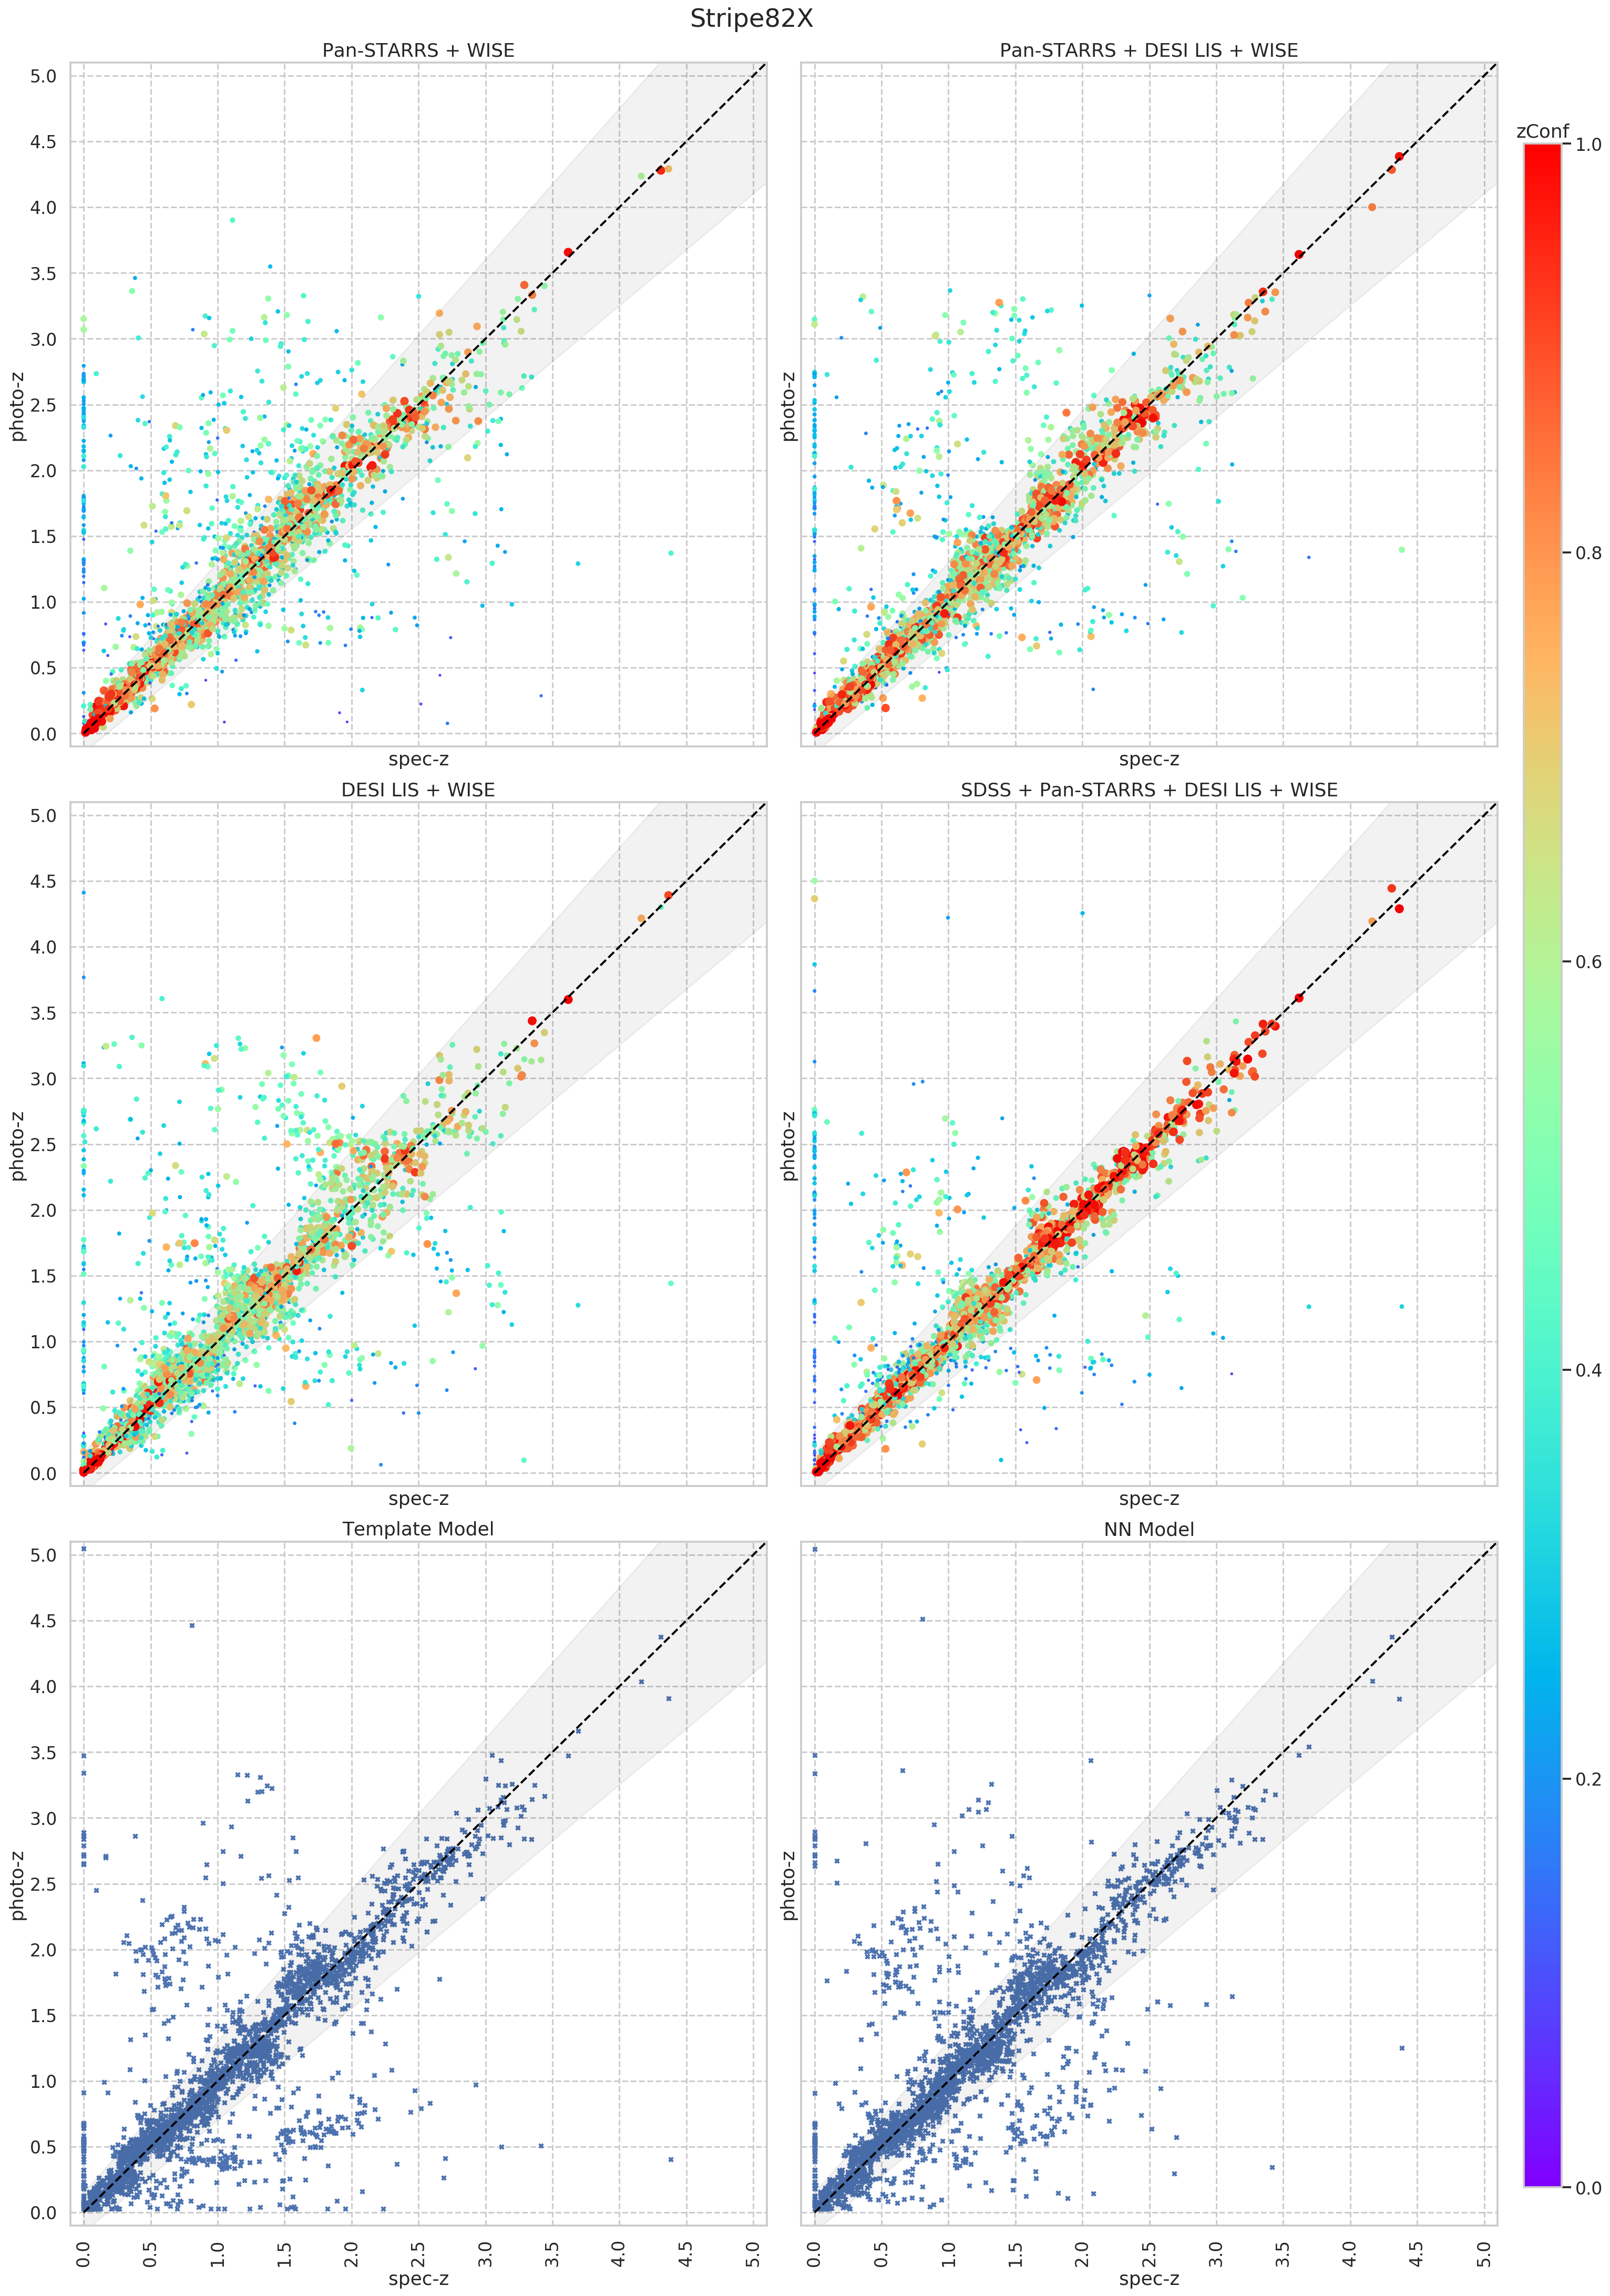
\includegraphics[width=0.9\linewidth]{images/scatterplots-stripe82x.png}
    \caption{Диаграммы рассеяния прогнозов четырех моделей Photo-z (Pan-STARRS + WISE слева сверху, Pan-STARRS + DESI LIS + WISE справа сверху, DESI LIS + WISE слева снизу и SDSS + PanSTARRS + DESI LIS + WISE справа снизу) на тестовой выборке рентгеновских объектов Stripe82X. По оси абсцисс -- значение spec-z, по оси ординат -- значение прогноза photo-z. Цветом и размером кружка показана мера достоверности прогноза zConf.}
    \label{fig:s82x}
\end{figure*}

\begin{figure*}
    \centering
    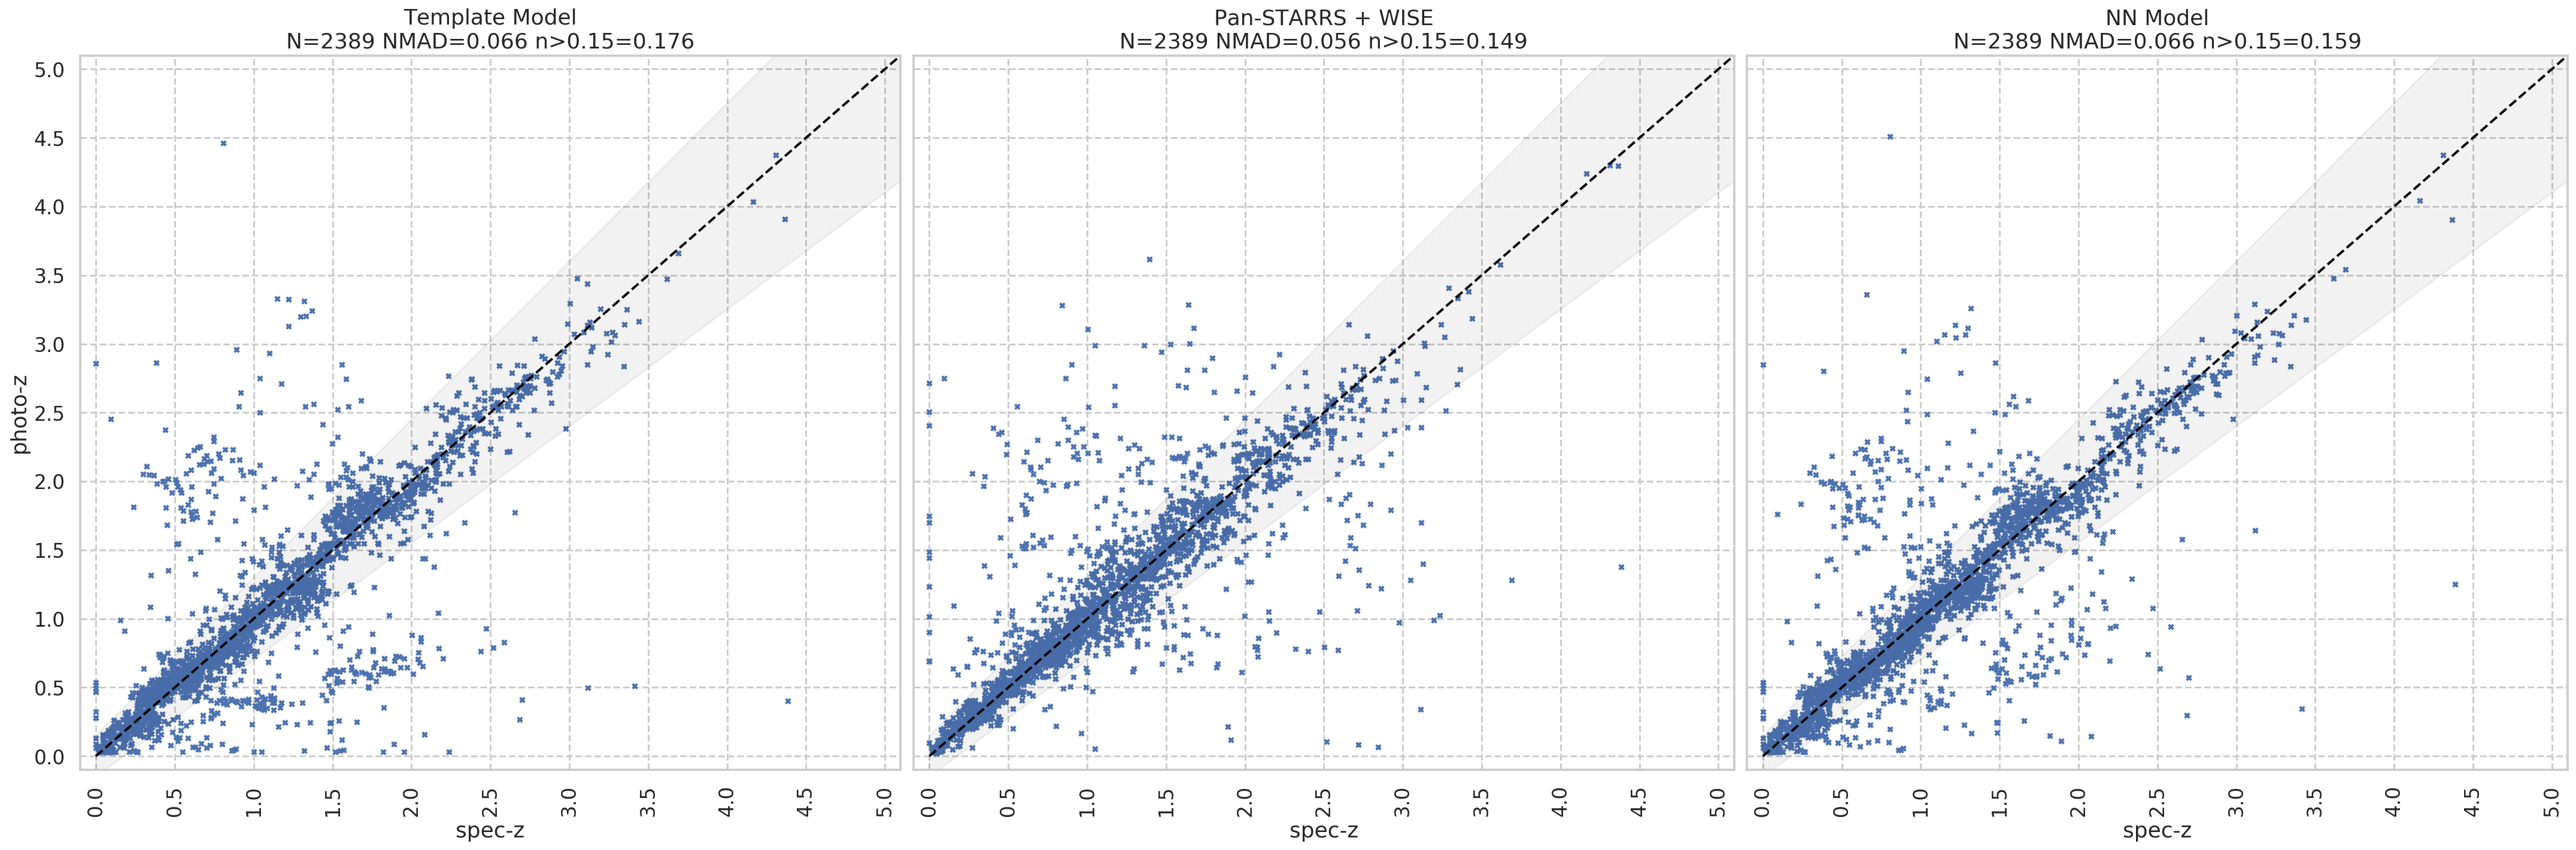
\includegraphics[width=0.9\linewidth]{images/scatterplots-stripe82x-sota19.png}
    \caption{Диаграммы рассеяния прогнозов для модели \ref{model:pw} + SOTA.}
    \label{fig:s82x-sota19}
\end{figure*}

\begin{figure*}
    \centering
    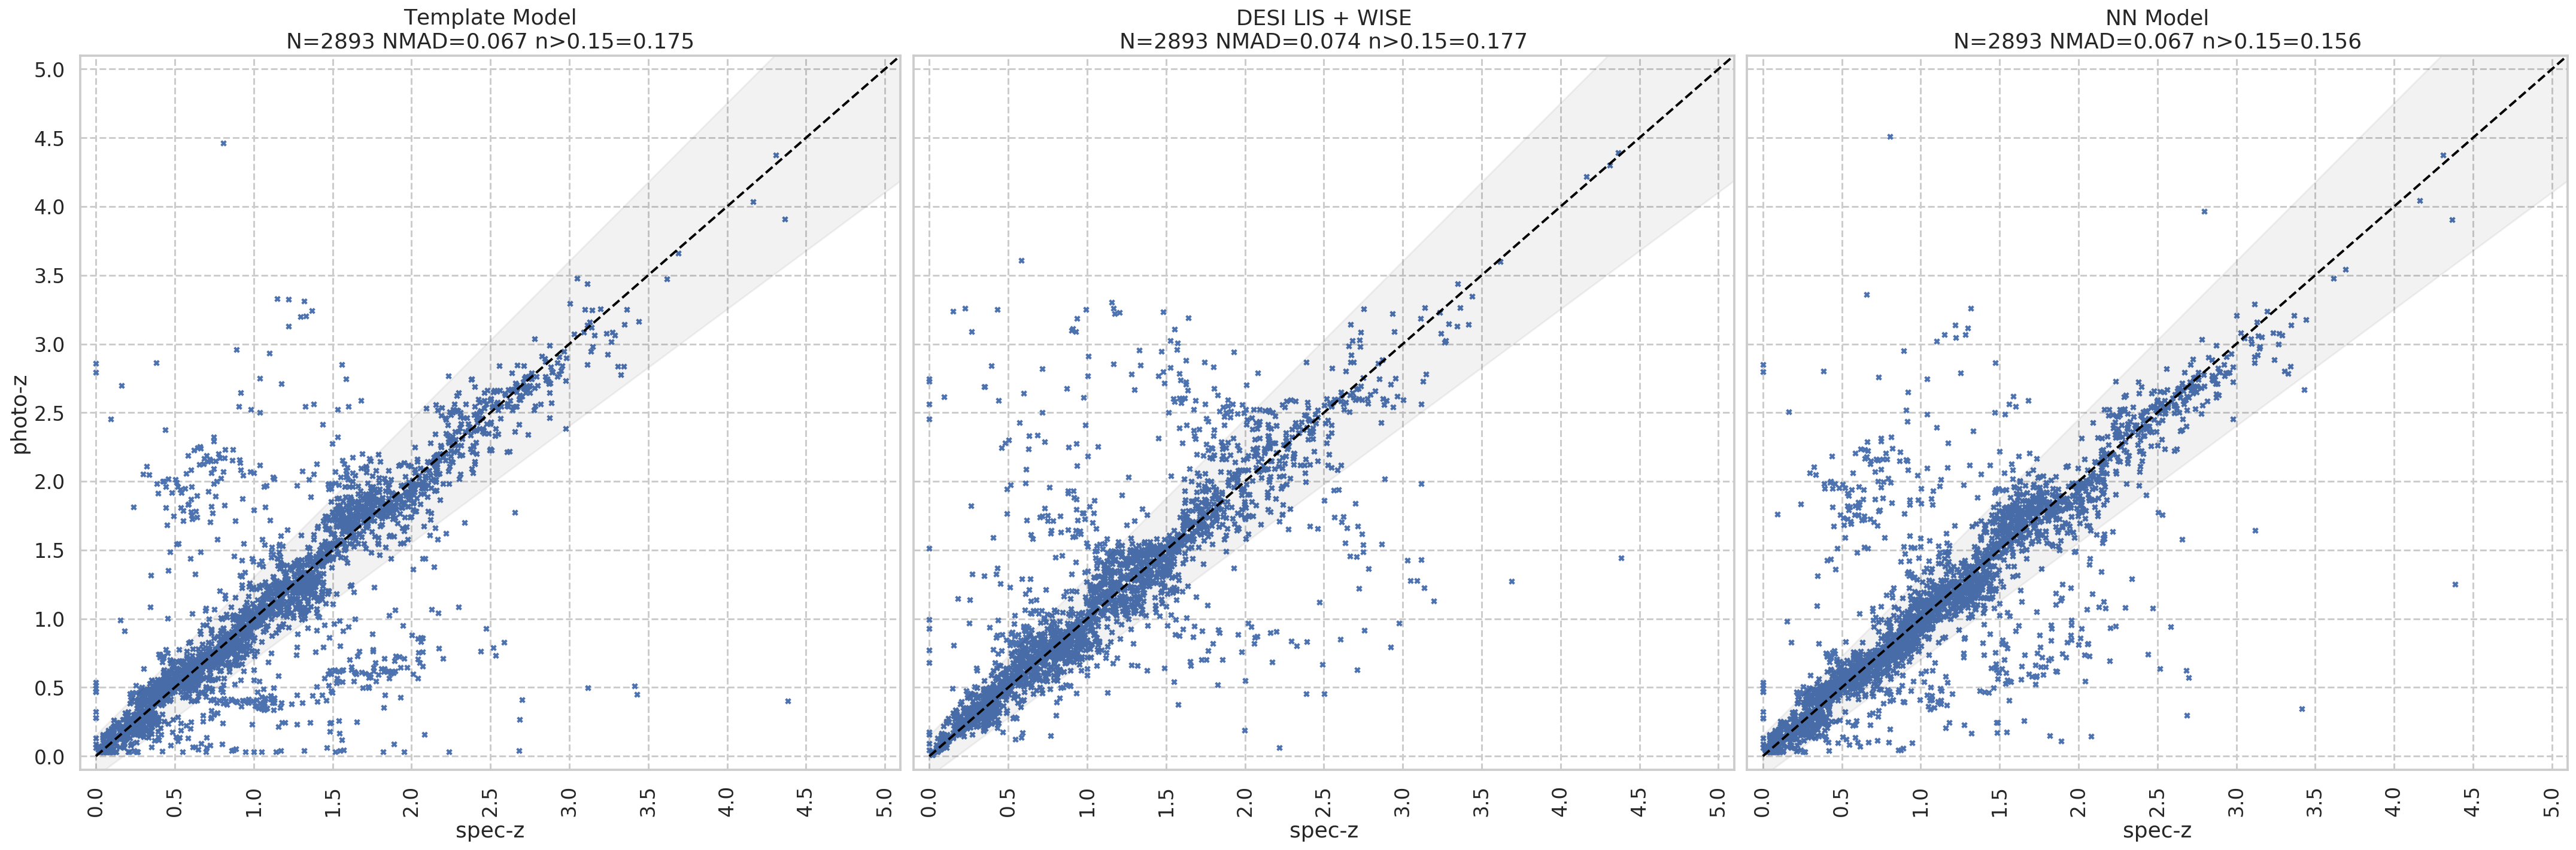
\includegraphics[width=0.9\linewidth]{images/scatterplots-stripe82x-sota22.png}
    \caption{Диаграммы рассеяния прогнозов для модели \ref{model:dw} + SOTA.}
    \label{fig:s82x-sota22}
\end{figure*}

\begin{figure*}
    \centering
    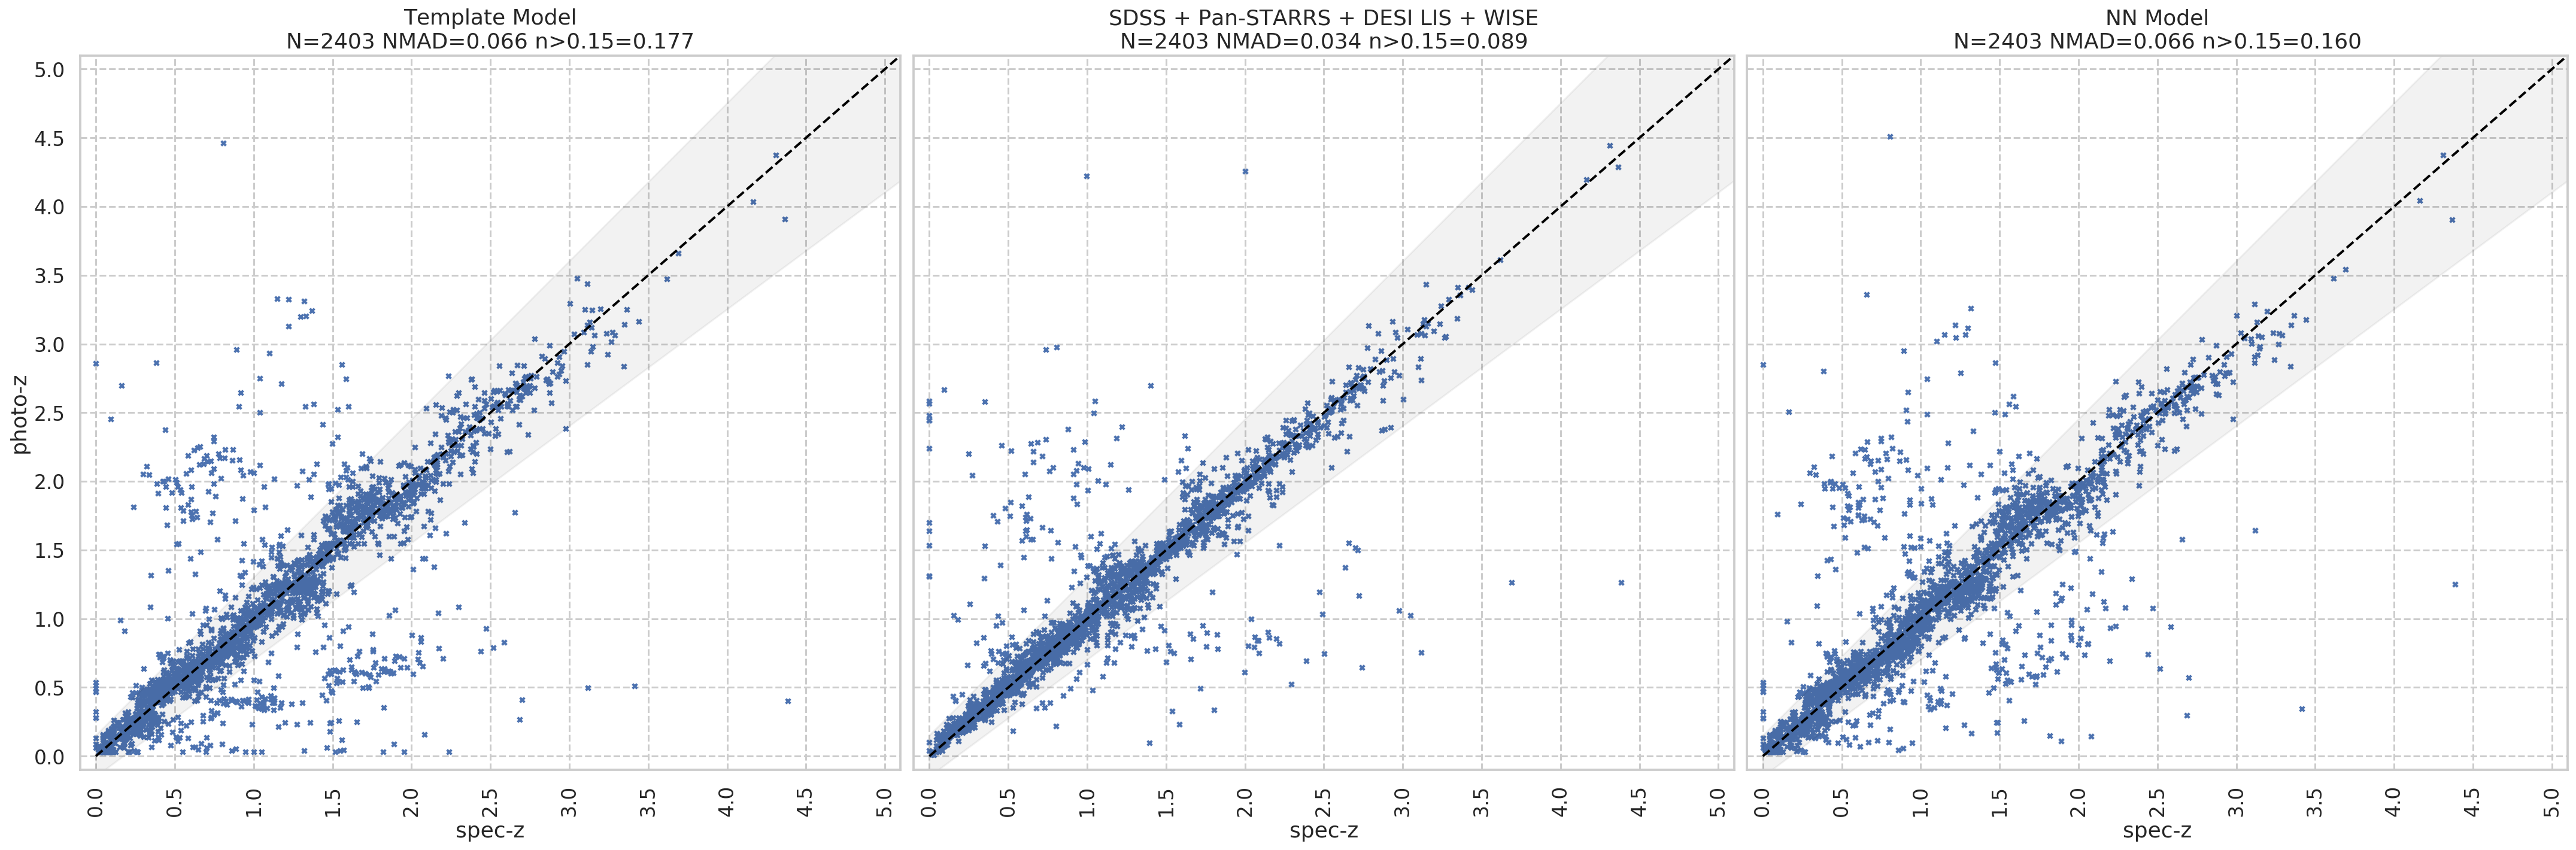
\includegraphics[width=0.9\linewidth]{images/scatterplots-stripe82x-sota35.png}
    \caption{Диаграммы рассеяния прогнозов для модели \ref{model:spdw} + SOTA.}
    \label{fig:s82x-sota35}
\end{figure*}

% \begin{table*}
% 	\begin{tabular}{llllllllll}
%             \hline
%             {} & \multicolumn{3}{l}{$All$ (2361 objects)} & \multicolumn{3}{l}{$z_{spec} < 0.5$ (563 objects)} & \multicolumn{3}{l}{$0.5 \leq z_{spec} < 1$ (629 objects)} \\
%             {} &               $NMAD$ &        $n>0.15$ & $C_{68} - 0.68$ &                         $NMAD$ &       $n>0.15$ &  $C_{68} - 0.68$ &                                $NMAD$ &        $n>0.15$ & $C_{68} - 0.68$ \\
%             Model          &                      &                 &                 &                                &                &                  &                                       &                 &                 \\
%             \hline
%             PW             &                0.056 &           0.148 &  \textbf{0.001} &                          0.037 &          0.083 &  \textbf{-0.017} &                                 0.053 &           0.145 &   \textbf{0.02} \\
%             PDW            &                0.045 &           0.109 &           0.077 &                          0.031 &          0.083 &            0.045 &                                 0.046 &           0.129 &           0.075 \\
%             DW             &                0.073 &           0.174 &          -0.007 &                          0.046 &           0.11 &            0.034 &                                 0.084 &           0.202 &          -0.025 \\
%             SPW            &                 0.04 &           0.105 &            0.089 &                          0.032 &          0.083 &           0.043 &                                 0.043 &           0.111 &            0.109 \\
%             SPDW           &       \textbf{0.034} &  \textbf{0.089} &           0.105 &                 \textbf{0.029} &  \textbf{0.08} &            0.068 &                        \textbf{0.038} &  \textbf{0.103} &           0.123 \\
%             Template Model &                0.065 &           0.175 &          -0.343 &                          0.075 &          0.112 &           -0.499 &                                 0.061 &           0.215 &          -0.287 \\
%             NN Model       &                0.066 &           0.158 &          -0.259 &                          0.072 &          0.114 &           -0.396 &                                 0.064 &           0.199 &          -0.192 \\
%             \hline
%             \end{tabular}
%             \caption{Точность моделей в зависимости от красного смещения (spec-z) на выборке Stripe82X для моделей Pan-STARRS + WISE (PW), Pan-STARRS + DESI LIS + WISE (PDW), DESI LIS + WISE (DW), SDSS + Pan-STARRS + DESI LIS + WISE (SPDW), шаблонной модели Ananna \ref{} (Template Model) и нейросетевой модели Brescia \ref{} (NN Model). Для каждого интервала даны метрики $NMAD$ \eqref{eq:nmad}, доля катастрофических выбросов $n_{.0.15}$ \eqref{eq:n015} и калибровка 68-процентных доверительных интервалов $C_{68} - 0.68$ \eqref{eq:c68}.}
% \end{table*}

% \begin{table*}
% 	\begin{tabular}{llllllllll}
%             \hline
%             {} & \multicolumn{3}{l}{$1 \leq z_{spec} < 1.5$ (507 objects)} & \multicolumn{3}{l}{$1.5 \leq z_{spec} < 2$ (363 objects)} & \multicolumn{3}{l}{$2 \leq z_{spec}$ (299 objects)} \\
%             {} &                                $NMAD$ &        $n>0.15$ &  $C_{68} - 0.68$ &                                $NMAD$ &        $n>0.15$ & $C_{68} - 0.68$ &                          $NMAD$ &        $n>0.15$ &  $C_{68} - 0.68$ \\
%             Model          &                                       &                 &                  &                                       &                 &                 &                                 &                 &                  \\
%             \hline
%             PW             &                                 0.079 &           0.174 &            0.018 &                                 0.076 &            0.16 &  \textbf{0.028} &                            0.07 &           0.217 &           -0.068 \\
%             PDW            &                                 0.061 &           0.105 &            0.071 &                                  0.04 &           0.099 &            0.13 &                           0.045 &           0.137 &            0.086 \\
%             DW             &                                 0.082 &           0.138 &  \textbf{-0.001} &                                 0.075 &           0.251 &           -0.03 &                           0.088 &           0.201 &  \textbf{-0.024} \\
%             SPW            &                                 0.053 &           0.108 &            0.097 &                                  0.04 &           0.096 &           0.163 &                           0.039 &            0.14 &            0.029 \\
%             SPDW           &                        \textbf{0.048} &  \textbf{0.089} &            0.119 &                        \textbf{0.031} &  \textbf{0.066} &           0.141 &                  \textbf{0.027} &  \textbf{0.104} &            0.073 \\
%             Template Model &                                  0.07 &           0.205 &           -0.287 &                                 0.074 &           0.218 &          -0.286 &                           0.046 &           0.107 &           -0.332 \\
%             NN Model       &                                 0.069 &           0.166 &           -0.209 &                                 0.066 &           0.182 &          -0.192 &                           0.047 &           0.117 &           -0.305 \\
%             \hline
%             \end{tabular}
%             \caption{Точность моделей в зависимости от красного смещения (spec-z) на выборке Stripe82X для моделей Pan-STARRS + WISE (PW), Pan-STARRS + DESI LIS + WISE (PDW), DESI LIS + WISE (DW), SDSS + Pan-STARRS + DESI LIS + WISE (SPDW), шаблонной модели Ananna \ref{} (Template Model) и нейросетевой модели Brescia \ref{} (NN Model). Для каждого интервала даны метрики $NMAD$ \eqref{eq:nmad}, доля катастрофических выбросов $n_{.0.15}$ \eqref{eq:n015} и калибровка 68-процентных доверительных интервалов $C_{68} - 0.68$ \eqref{eq:c68}.}
% \end{table*}




% \begin{table*}
% 	\begin{tabular}{llllllllll}
%             \hline
%             {} & \multicolumn{3}{l}{$z_{mag} < 19$ (520 objects)} & \multicolumn{3}{l}{$19 \leq z_{mag} < 20$ (604 objects)} & \multicolumn{3}{l}{$20 \leq z_{mag} < 20.5$ (403 objects)} \\
%             {} &                       $NMAD$ &        $n>0.15$ & $C_{68} - 0.68$ &                               $NMAD$ &        $n>0.15$ & $C_{68} - 0.68$ &                                 $NMAD$ &        $n>0.15$ & $C_{68} - 0.68$ \\
%             Model          &                              &                 &                 &                                      &                 &                 &                                        &                 &                 \\
%             \hline
%             PW             &                        0.037 &           0.046 &          -0.034 &                                0.042 &           0.073 &           0.063 &                                  0.064 &           0.134 &  \textbf{0.012} \\
%             PDW            &                        0.027 &            0.04 &           0.045 &                                0.036 &           0.065 &           0.116 &                                  0.046 &           0.102 &           0.107 \\
%             DW             &                        0.039 &           0.083 &  \textbf{0.024} &                                0.068 &           0.111 &  \textbf{0.015} &                                  0.076 &           0.156 &  \textbf{0.012} \\
%             SPW            &               \textbf{0.024} &           0.038 &           0.062 &                                0.031 &           0.045 &           0.115 &                                  0.041 &           0.087 &           0.104 \\
%             SPDW           &               \textbf{0.024} &  \textbf{0.029} &           0.082 &                       \textbf{0.028} &  \textbf{0.041} &           0.131 &                         \textbf{0.033} &  \textbf{0.074} &           0.107 \\
%             Template Model &                        0.061 &           0.092 &          -0.536 &                                0.062 &           0.144 &          -0.399 &                                  0.064 &           0.166 &           -0.38 \\
%             NN Model       &                        0.062 &           0.092 &          -0.463 &                                0.058 &           0.132 &          -0.309 &                                  0.061 &           0.144 &          -0.288 \\
%             \hline
%             \end{tabular}
%             \caption{Точность моделей в зависимости от величины в фильтре $z$ на выборке Stripe82X для моделей Pan-STARRS + WISE (PW), Pan-STARRS + DESI LIS + WISE (PDW), DESI LIS + WISE (DW), SDSS + Pan-STARRS + DESI LIS + WISE (SPDW), шаблонной модели Ananna \ref{} (Template Model) и нейросетевой модели Brescia \ref{} (NN Model). Для каждого интервала даны метрики $NMAD$ \eqref{eq:nmad}, доля катастрофических выбросов $n_{.0.15}$ \eqref{eq:n015} и калибровка 68-процентных доверительных интервалов $C_{68} - 0.68$ \eqref{eq:c68}.}
% \end{table*}

% \begin{table*}
% 	\begin{tabular}{lllllll}
%             \hline
%             {} & \multicolumn{3}{l}{$20.5 \leq z_{mag} < 21$ (356 objects)} & \multicolumn{3}{l}{$21 \leq z_{mag} < 23$ (476 objects)} \\
%             {} &                                 $NMAD$ &        $n>0.15$ &  $C_{68} - 0.68$ &                               $NMAD$ &        $n>0.15$ & $C_{68} - 0.68$ \\
%             Model          &                                        &                 &                  &                                      &                 &                 \\
%             \hline
%             PW             &                                  0.077 &           0.202 &  \textbf{-0.009} &                                0.123 &           0.321 &          -0.041 \\
%             PDW            &                                  0.056 &           0.121 &            0.073 &                                0.082 &           0.239 &  \textbf{0.038} \\
%             DW             &                                  0.088 &           0.219 &           -0.011 &                                0.119 &           0.334 &          -0.081 \\
%             SPW            &                                  0.054 &           0.126 &            0.076 &                                0.082 &           0.252 &            0.085 \\
%             SPDW           &                         \textbf{0.044} &  \textbf{0.107} &            0.107 &                       \textbf{0.064} &  \textbf{0.214} &           0.095 \\
%             Template Model &                                  0.057 &           0.199 &           -0.217 &                                0.087 &           0.294 &           -0.13 \\
%             NN Model       &                                  0.062 &           0.169 &           -0.132 &                                0.089 &           0.269 &          -0.043 \\
%             \hline
%             \end{tabular}
%             \caption{Точность моделей в зависимости от величины в фильтре $z$ на выборке Stripe82X для моделей Pan-STARRS + WISE (PW), Pan-STARRS + DESI LIS + WISE (PDW), DESI LIS + WISE (DW), SDSS + Pan-STARRS + DESI LIS + WISE (SPDW), шаблонной модели Ananna \ref{} (Template Model) и нейросетевой модели Brescia \ref{} (NN Model). Для каждого интервала даны метрики $NMAD$ \eqref{eq:nmad}, доля катастрофических выбросов $n_{.0.15}$ \eqref{eq:n015} и калибровка 68-процентных доверительных интервалов $C_{68} - 0.68$ \eqref{eq:c68}.}
% \end{table*}

\begin{table*}
	\begin{tabular}{llllllllll}
            \hline
            {} & \multicolumn{3}{l}{$FSoft < 1e-14$ (951 objects)} & \multicolumn{3}{l}{$FSoft < 4e-14$ (2016 objects)} & \multicolumn{3}{l}{$FSoft < 1.0$ (2223 objects)} \\
            {} &                        $NMAD$ &        $n>0.15$ & $C_{68} - 0.68$ &                         $NMAD$ &        $n>0.15$ &  $C_{68} - 0.68$ &                       $NMAD$ &        $n>0.15$ &  $C_{68} - 0.68$ \\
            Model            &                               &                 &                 &                                &                 &                  &                              &                 &                  \\
            \hline
            \ref{model:pw}   &                         0.068 &           0.188 &           0.016 &                          0.058 &           0.154 &            0.026 &                        0.056 &           0.148 &            0.026 \\
            \ref{model:pdw}  &                         0.049 &           0.127 &           0.084 &                          0.047 &           0.113 &             0.08 &                        0.045 &           0.108 &             0.08 \\
            \ref{model:dw}   &                         0.073 &           0.196 &  \textbf{0.005} &                          0.073 &           0.176 &  \textbf{-0.006} &                        0.073 &           0.172 &  \textbf{-0.011} \\
            \ref{model:spw}  &                         0.048 &           0.138 &           0.079 &                          0.042 &            0.11 &            0.091 &                         0.04 &           0.105 &            0.092 \\
            \ref{model:spdw} &                \textbf{0.038} &  \textbf{0.107} &             0.1 &                 \textbf{0.035} &  \textbf{0.092} &            0.109 &               \textbf{0.033} &  \textbf{0.088} &             0.11 \\
            Template Model   &                         0.061 &           0.161 &          -0.284 &                          0.064 &            0.17 &           -0.324 &                        0.064 &           0.175 &           -0.339 \\
            NN Model         &                         0.063 &           0.145 &          -0.199 &                          0.065 &           0.153 &           -0.243 &                        0.065 &           0.159 &           -0.256 \\
            \hline
            \end{tabular}
            \caption{Точность моделей в зависимости от рентгеновского потока (FSoft) на выборке Stripe82X для моделей Pan-STARRS + WISE (PW), Pan-STARRS + DESI LIS + WISE (PDW), DESI LIS + WISE (DW), SDSS + Pan-STARRS + DESI LIS + WISE (SPDW), шаблонной модели Ananna \ref{} (Template Model) и нейросетевой модели Brescia \ref{} (NN Model). Для каждого интервала даны метрики $NMAD$ \eqref{eq:nmad}, доля катастрофических выбросов $n_{.0.15}$ \eqref{eq:n015} и калибровка 68-процентных доверительных интервалов $C_{68} - 0.68$ \eqref{eq:c68}.}
\end{table*}

\subsection{PDZ reliability}

\begin{figure*}
    \centering
    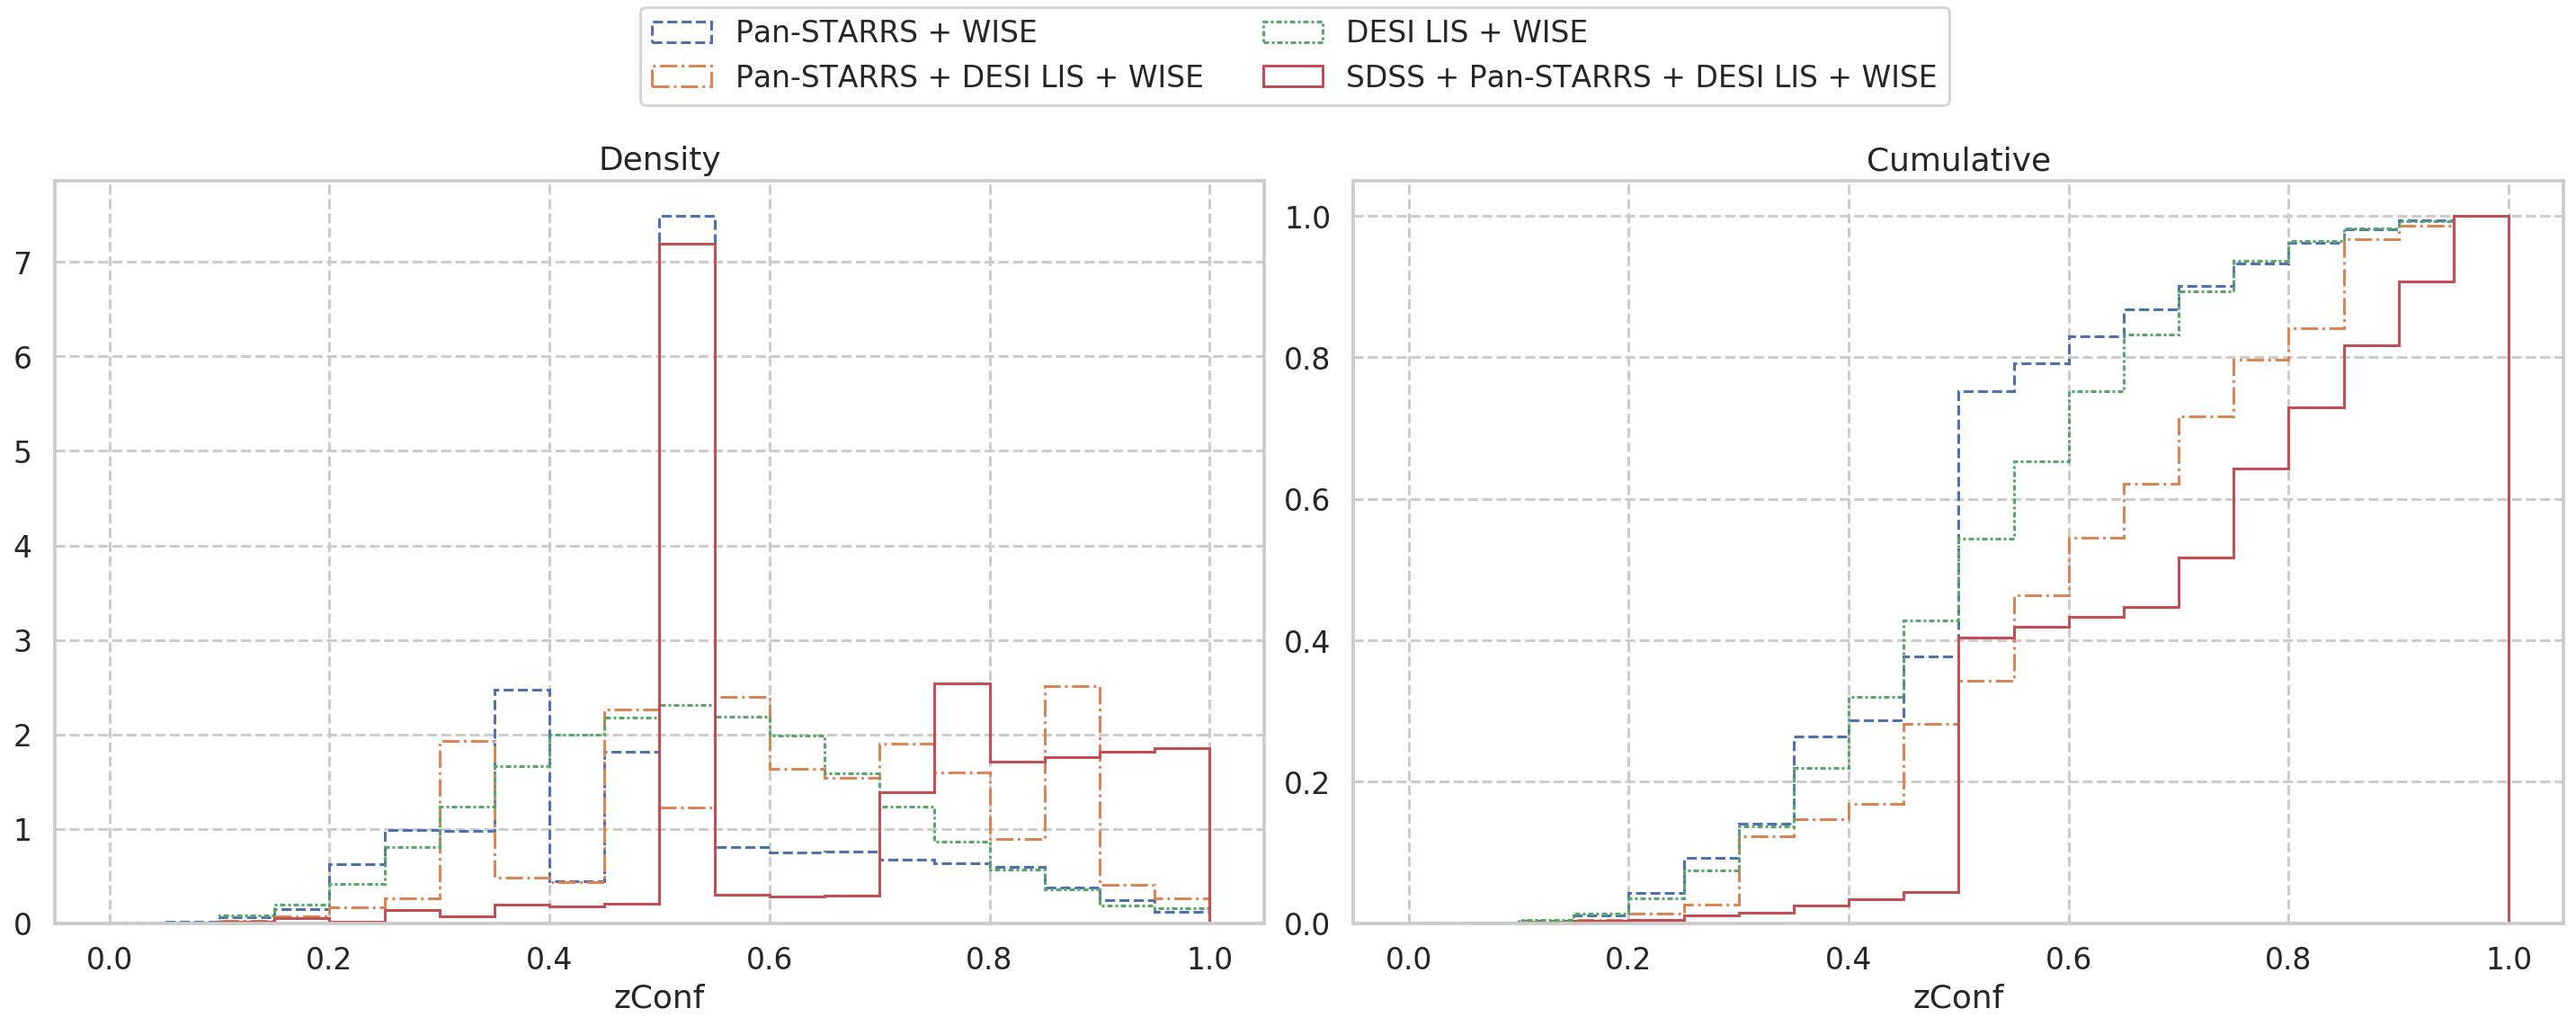
\includegraphics[width=0.9\linewidth]{images/zconf-cal-dr16q.png}
    \caption{zConf distribution on DR16q test sample}
    \label{fig:zconf-cal-dr16q}
\end{figure*}

\begin{figure*}
    \centering
    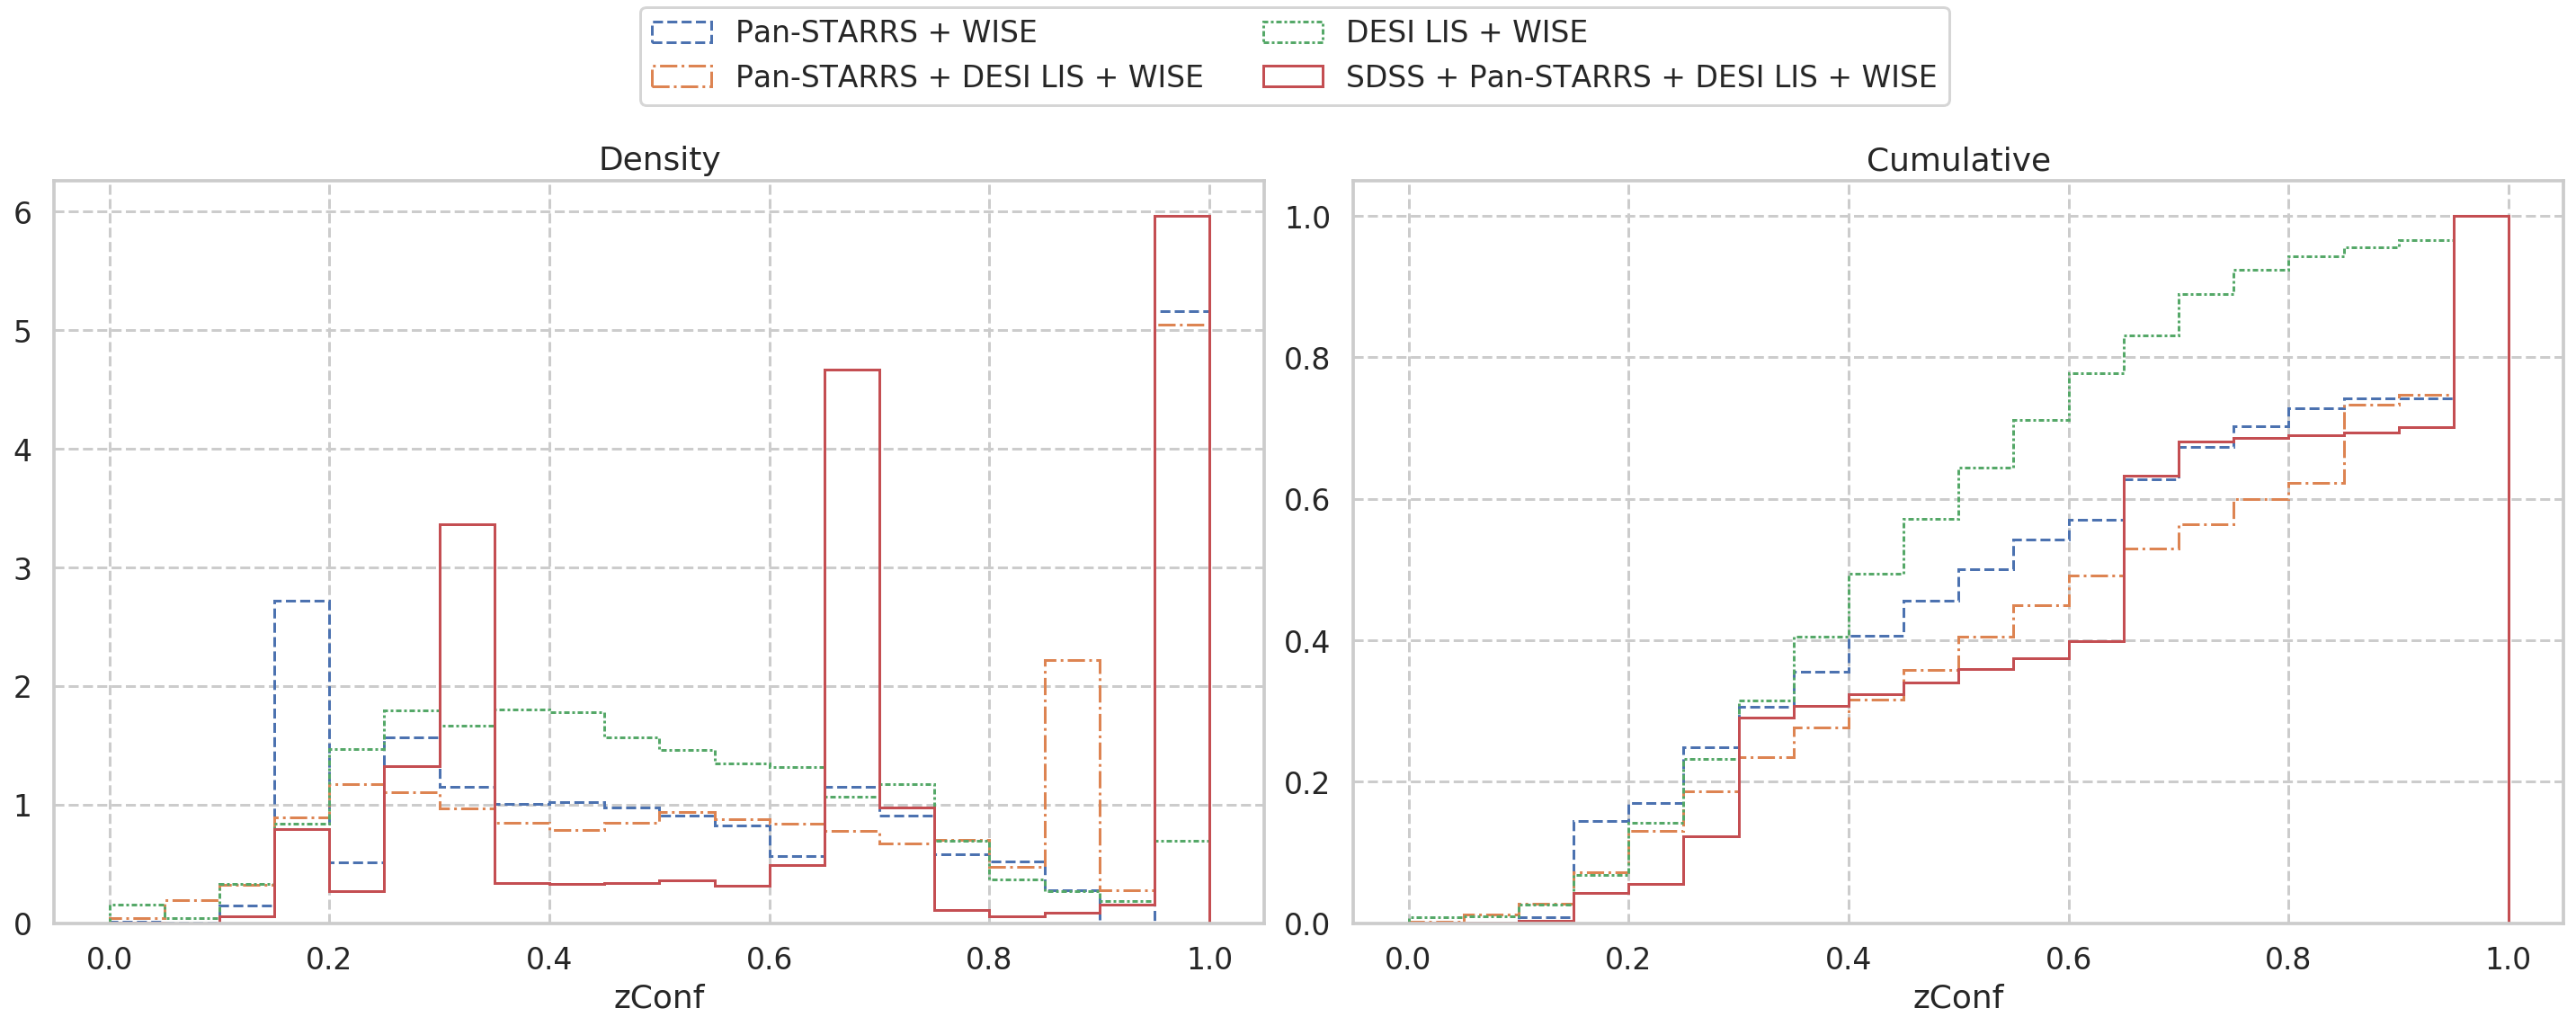
\includegraphics[width=0.9\linewidth]{images/zconf-cal-stripe82X.png}
    \caption{zConf distribution on Stripe82X test sample}
    \label{fig:zconf-cal-stripe82X}
\end{figure*}

% ===============================================================================
% ===============================================================================
% ===============================================================================

\section{Conclusion}

% В рамках работы было построено множество моделей photo-z на основе различных признаков, которые строятся по данным трех современных фотометрических обзоров~--- SDSS, Pan-STARRS1 и DESI Legacy Imaging Survey. Обучающая выборка состоит из $\sim$580000 оптических квазаров и галактик и сбалансирована, чтобы аппроксимировать распределение рентгеновских объектов. Разметка взята из спектрального каталога оптических объектов SDSS.

% На тестовой выборке рентгеновских объектов поля Stripe82X \cite{bib:ananna}, за счет использования данных всех трех вышеупомянутых обзоров, была достигнута точность по метрикам $NMAD$ и доля выбросов $n_{>0.15}$ значительно выше (почти в 2 раза), чем точность лучших моделей известных в литературе (SOTA), что является основным результатом работы. Для лучшей модели / шаблонной модели \cite{bib:ananna} / нейросетевой модели \cite{bib:brescia} на выборке Stripe82X получены значения метрик $NMAD$ = 0.034 / 0.065 / 0.066 и $n_{>0.15}$ = 0.088 / 0.170 / 0.156, соответственно.

The proposed photo-z models based on Random Forests show accuracy (up to 2 times) better than current SOTA results in the literature (on Stripe82X field). The main accuracy improvement comes from using a large training sample ($\sim$600k objects) with features from modern wide photometric surveys. First optical spectroscopic observations of eRosita sources show that the proposed photo-z models are effective in the ongoing search for distant X-ray quasars (see e.g. \citep{2020MNRAS.497.1842M,2020AstL...46..149K,2020AstL...46..429D}).

The presented photo-z models are integrated into the SRGz system designed to construct a three-dimensional map of X-ray sources on the Eastern Galactic Hemisphere of the SRG/eRosita All-Sky survey. The SRGz system is developed in the science working group of RU eROSITA consortium on X-ray source detection, identification, and eROSITA source catalog in the High Energy Astrophysics Department at Space Research Institute of the Russian Academy of Sciences.

% ===============================================================================
% ===============================================================================
% ===============================================================================

\section{Discussion}

Провалы в точности по zspec. Переход на ансамбли нейронных сетей. Источник данных о поглощении на всем небе?

\section*{Acknowledgments}
..

% bibliograpgy 
\bibliographystyle{mnras}
\bibliography{main}

\appendix

\section{Advanced metrics charts}

\begin{landscape}
\begin{figure}
    \centering
    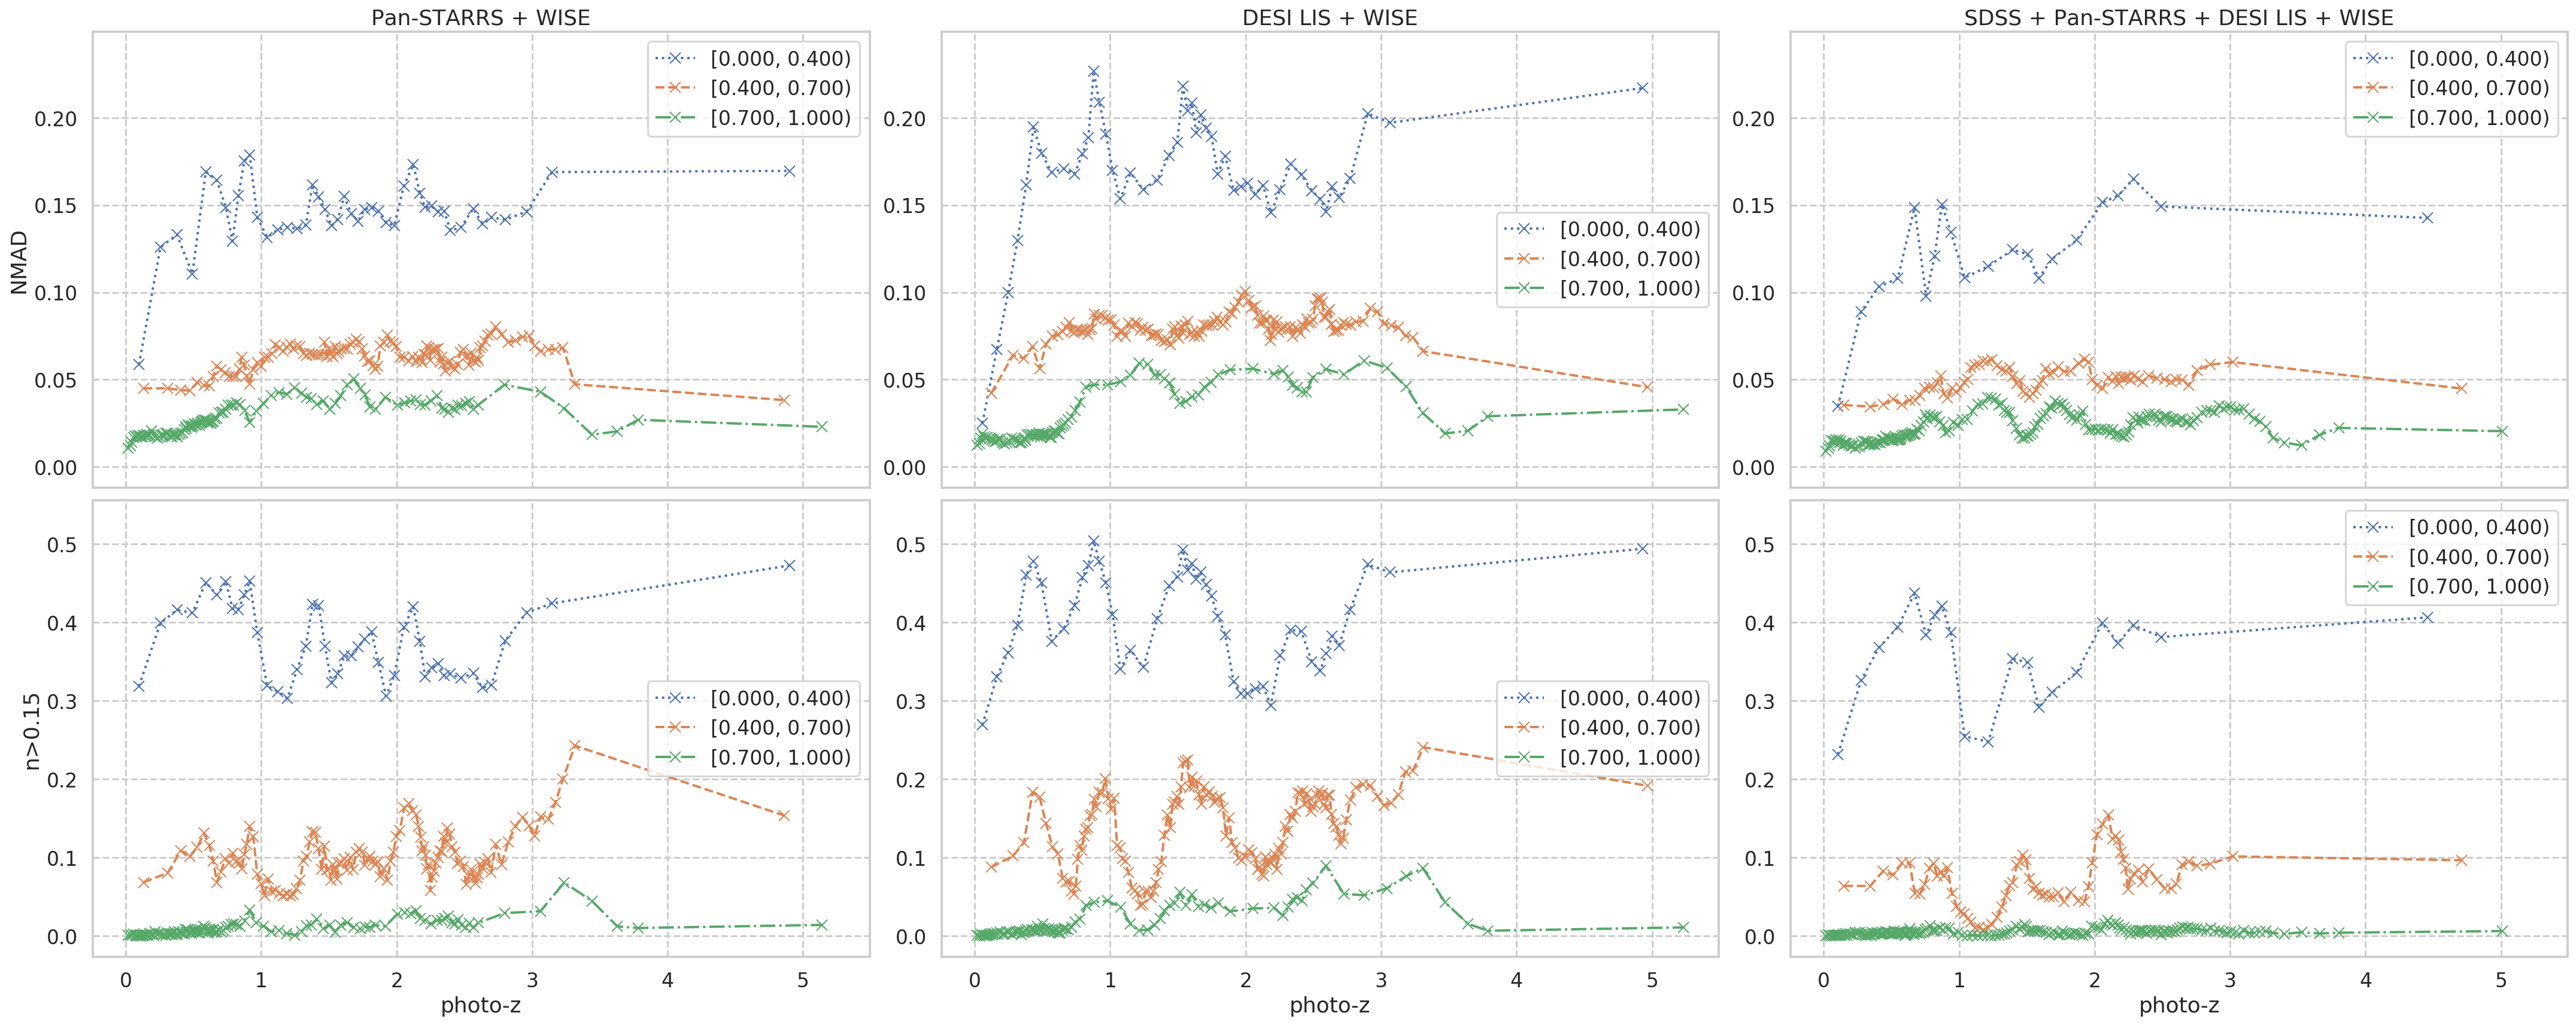
\includegraphics[width=25cm]{images/metrics-adv-photoz-x-zconf-cv2.png}
    \caption{Метрики в зависимости от photo-z для разных порогов по zConf на кросс-валидации}
    \label{fig:my_label}
\end{figure}
\end{landscape}


\begin{landscape}
\begin{figure}
    \centering
    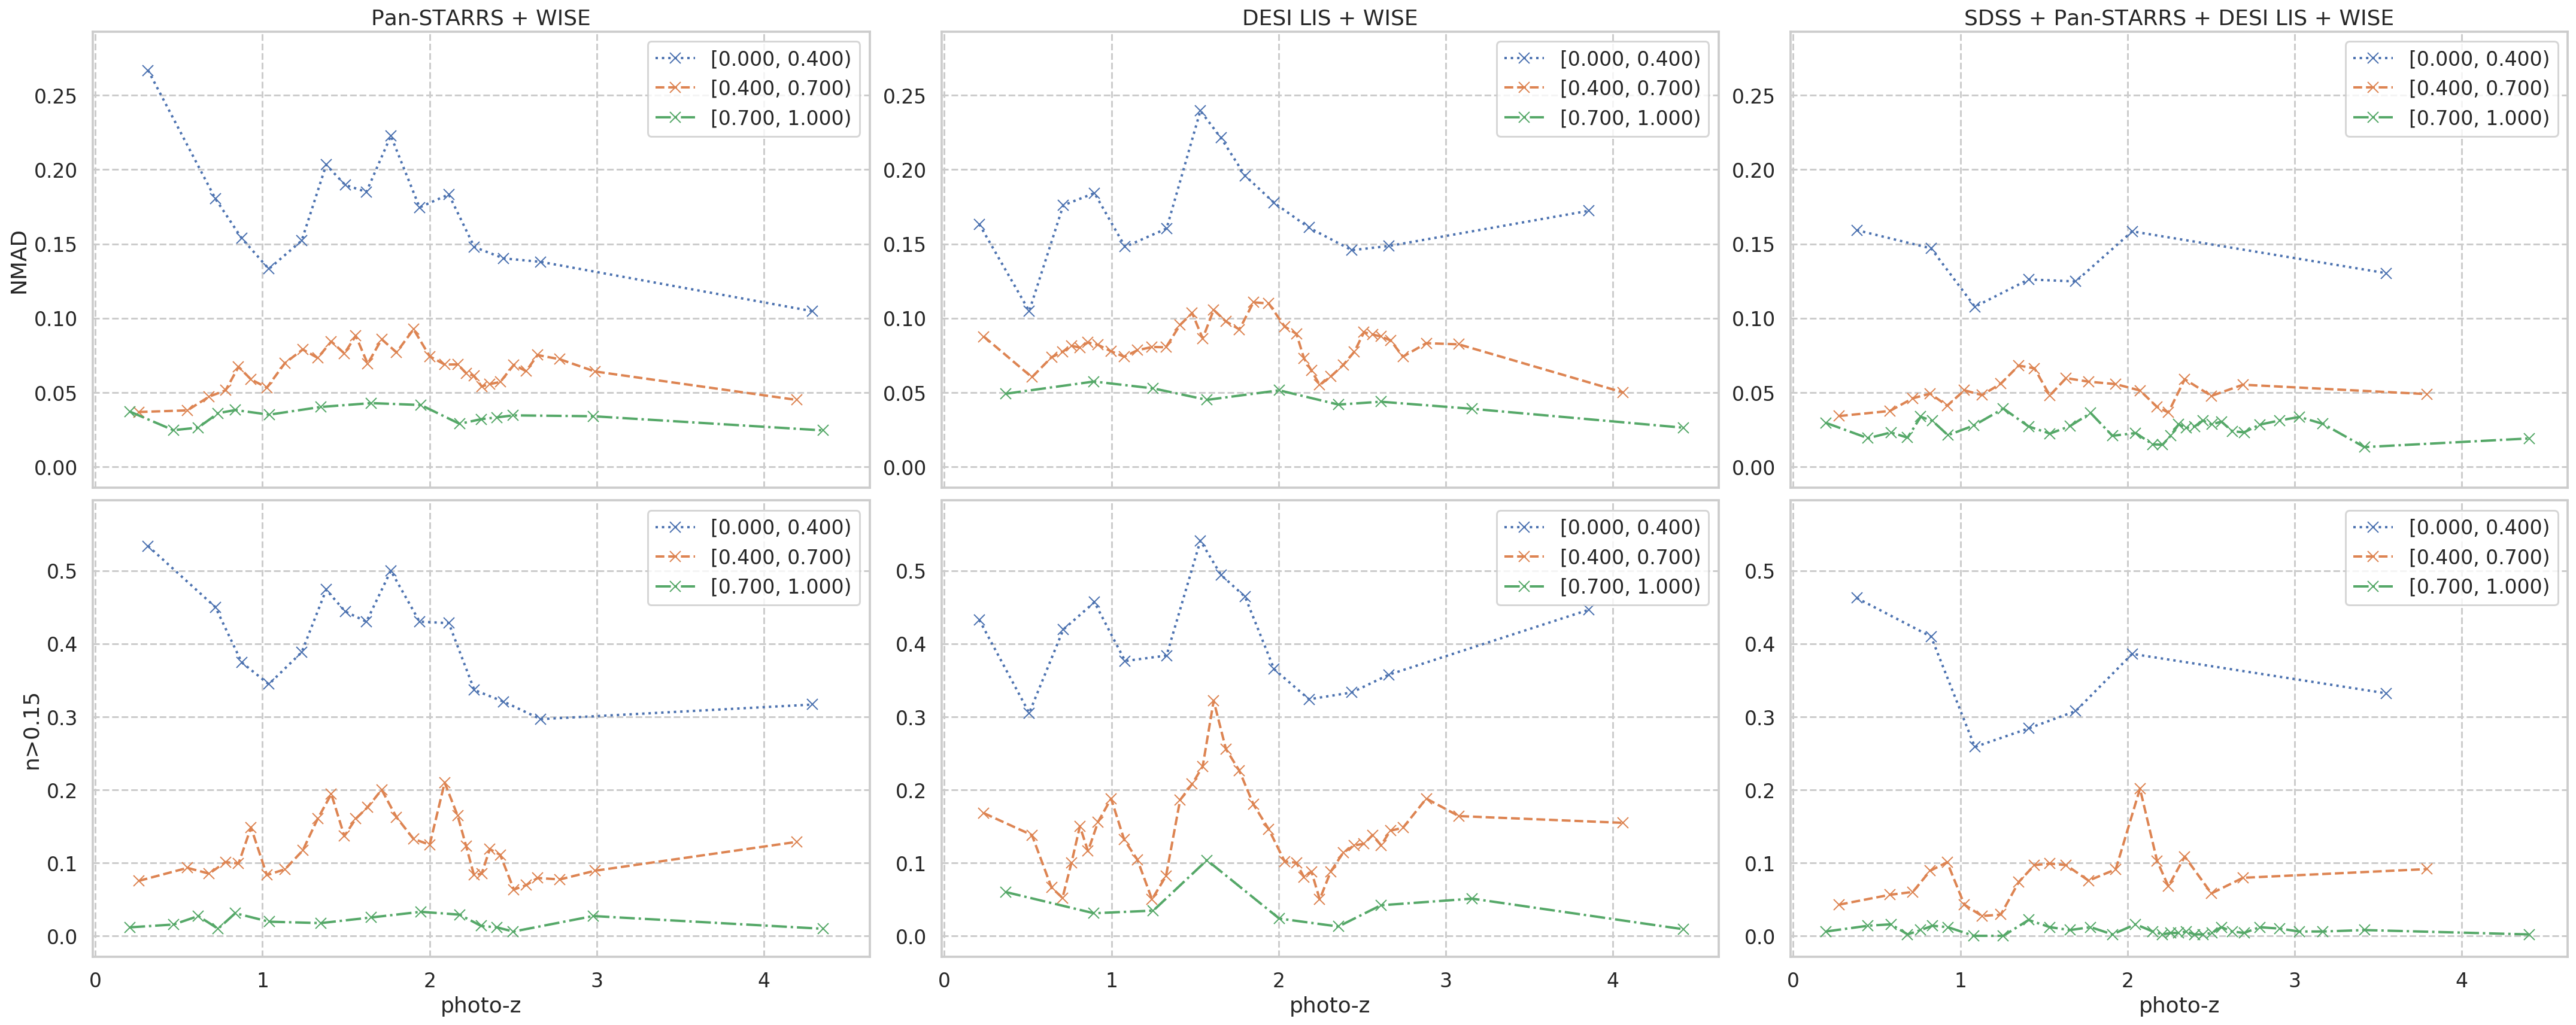
\includegraphics[width=0.9\linewidth]{images/metrics-adv-photoz-x-zconf-dr16q.png}
    \caption{Метрики в зависимости от photo-z для разных порогов по zConf на DR16q}
    \label{fig:my_label}
\end{figure}
\end{landscape}


\begin{landscape}
\begin{figure}
    \centering
    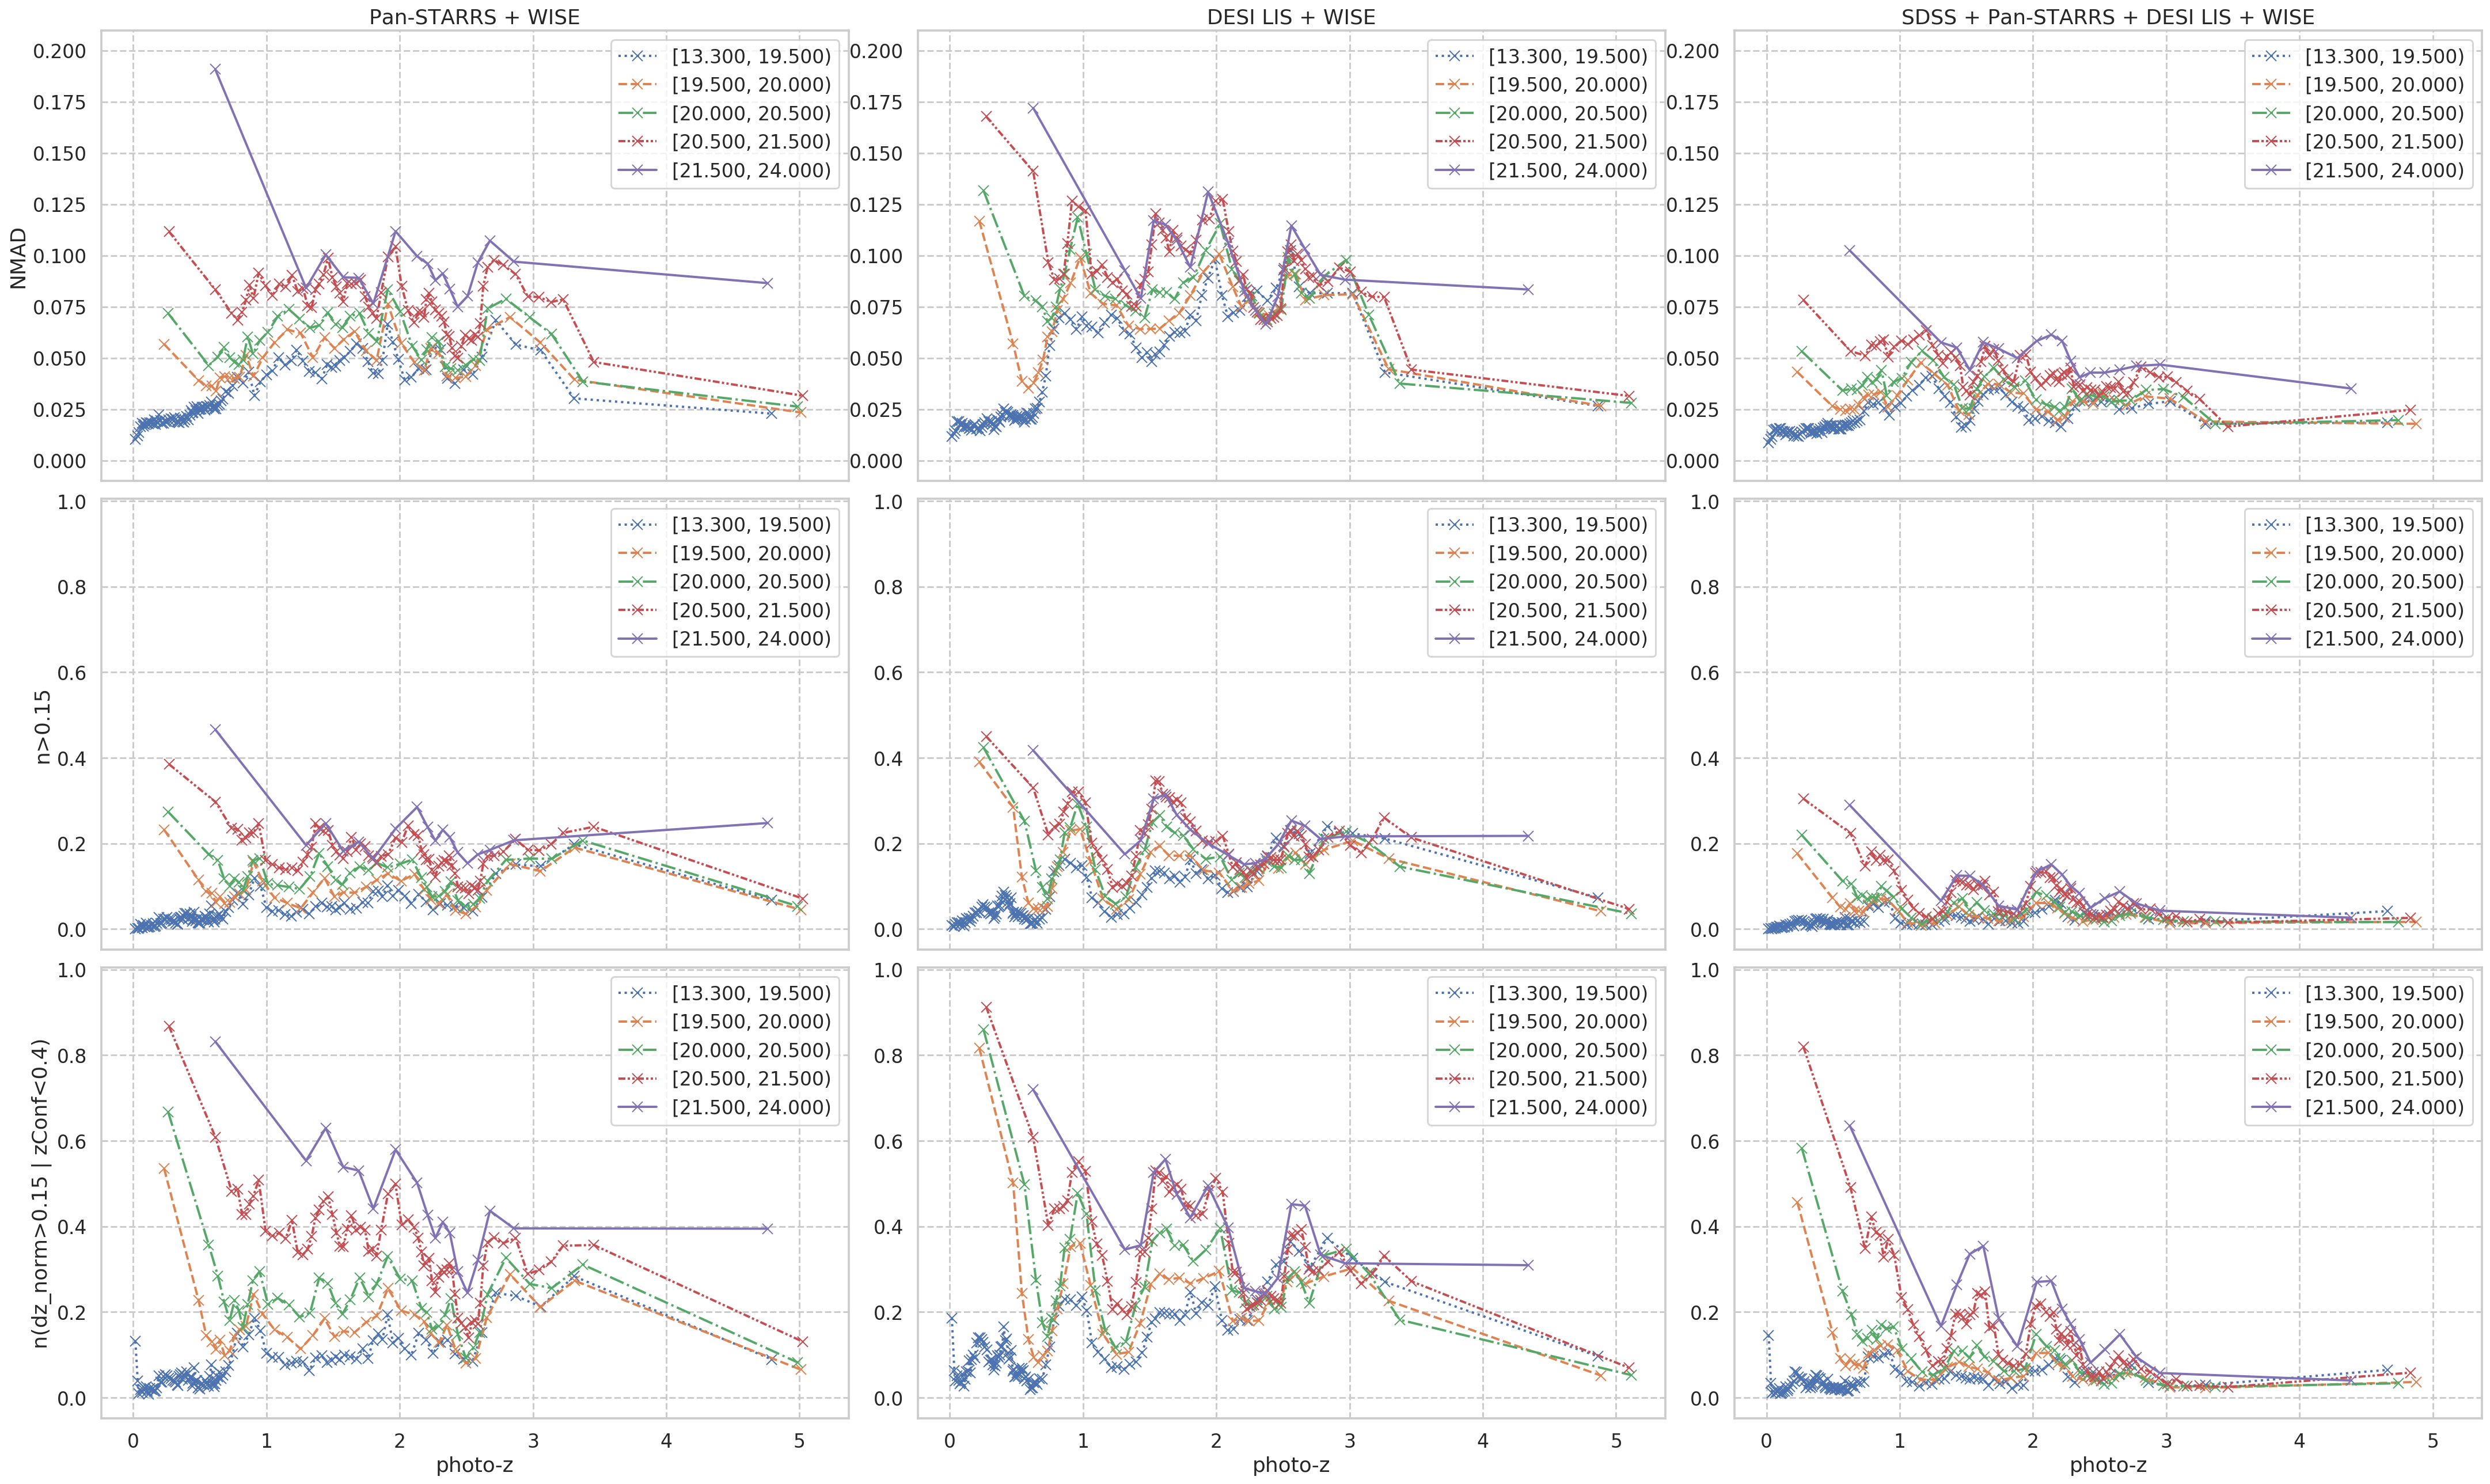
\includegraphics[width=0.9\linewidth]{images/metrics-adv-photoz-x-zmag-cv2.png}
    \caption{Метрики в зависимости от photo-z для разных порогов по $z_mag$ на кросс-валидации}
    \label{fig:my_label}
\end{figure}
\end{landscape}


\begin{landscape}
\begin{figure}
    \centering
    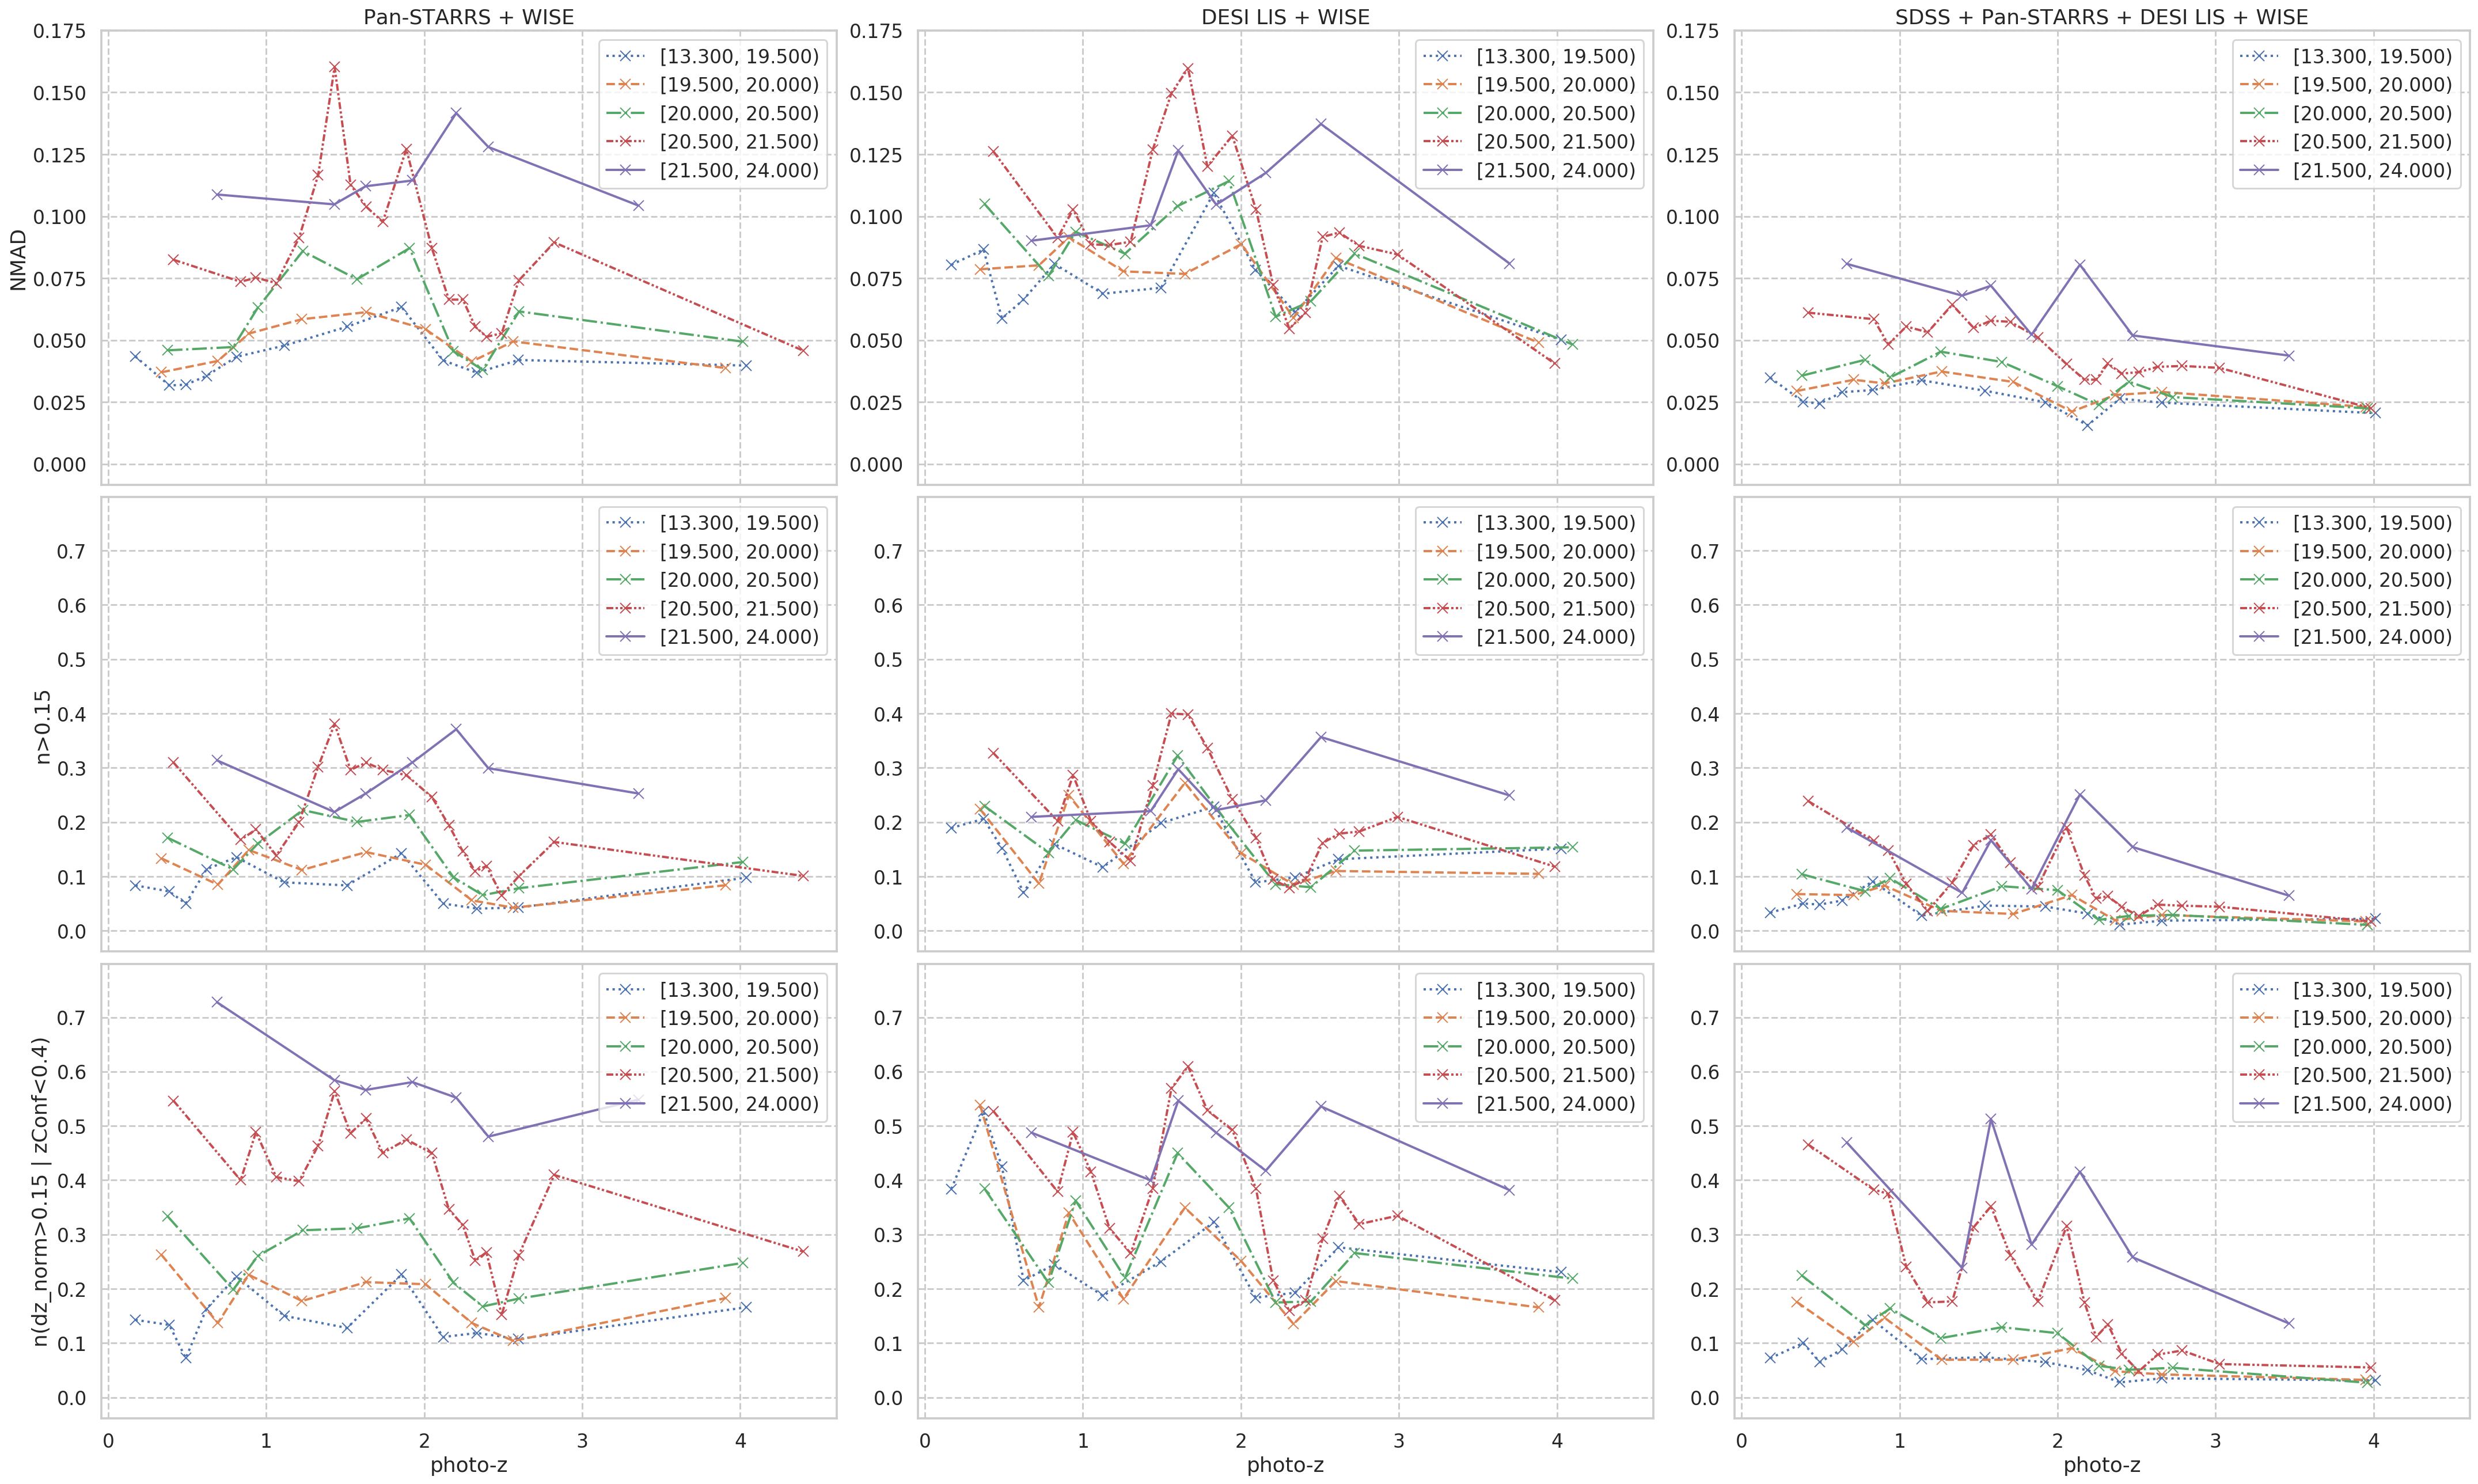
\includegraphics[width=0.9\linewidth]{images/metrics-adv-photoz-x-zmag-dr16q.png}
    \caption{Метрики в зависимости от photo-z для разных порогов по $z_mag$ на DR16q}
    \label{fig:my_label}
\end{figure}
\end{landscape}


\begin{landscape}
\begin{figure}
    \centering
    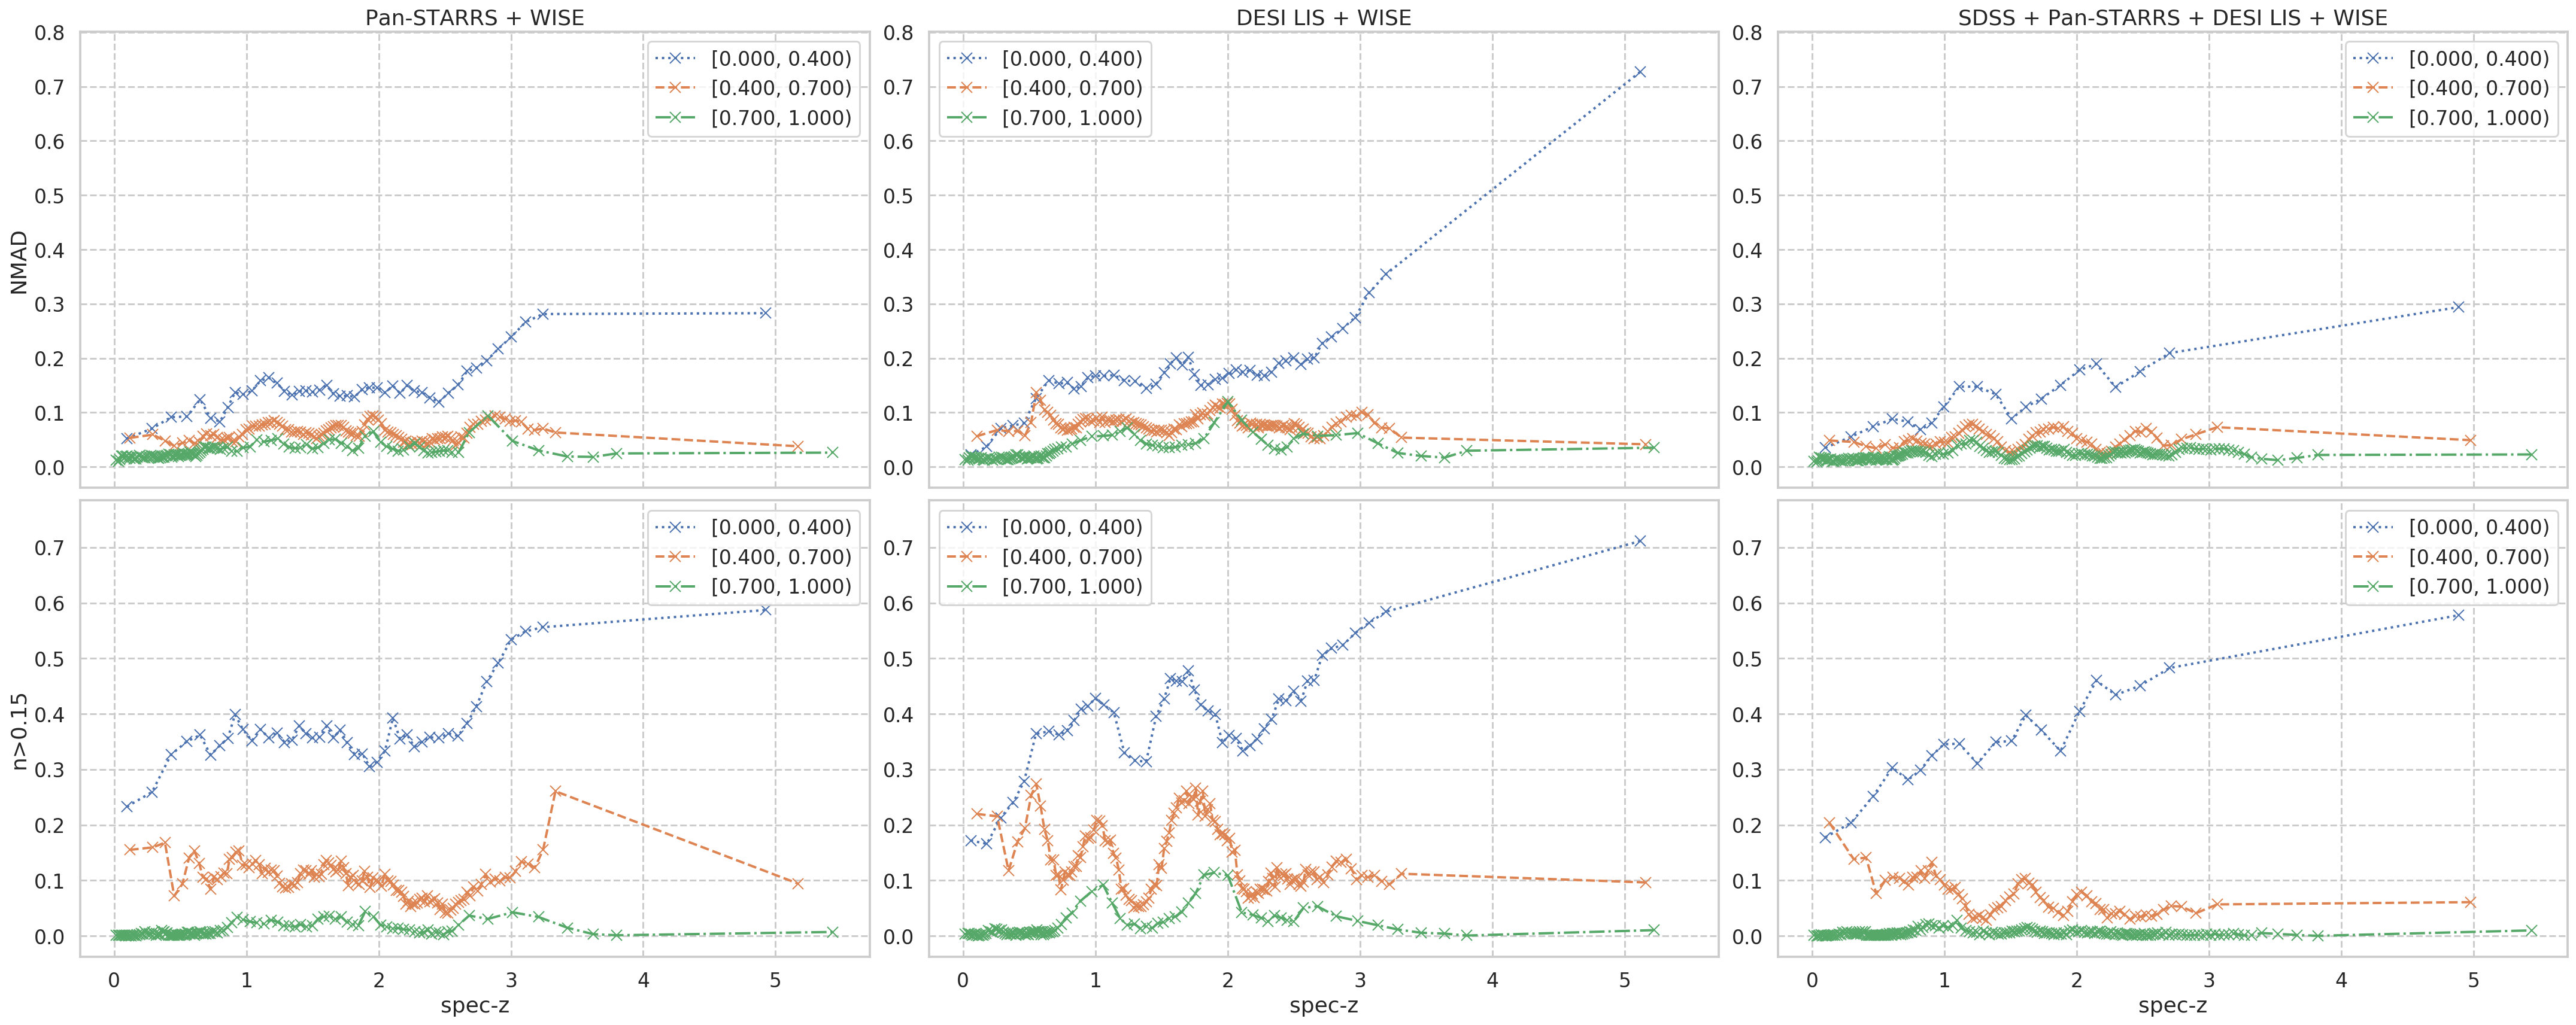
\includegraphics[width=0.9\linewidth]{images/metrics-adv-zspec-x-zconf-cv2.png}
    \caption{Метрики в зависимости от spec-z для разных порогов по zConf на кросс-валидации}
    \label{fig:my_label}
\end{figure}
\end{landscape}


\begin{landscape}
\begin{figure}
    \centering
    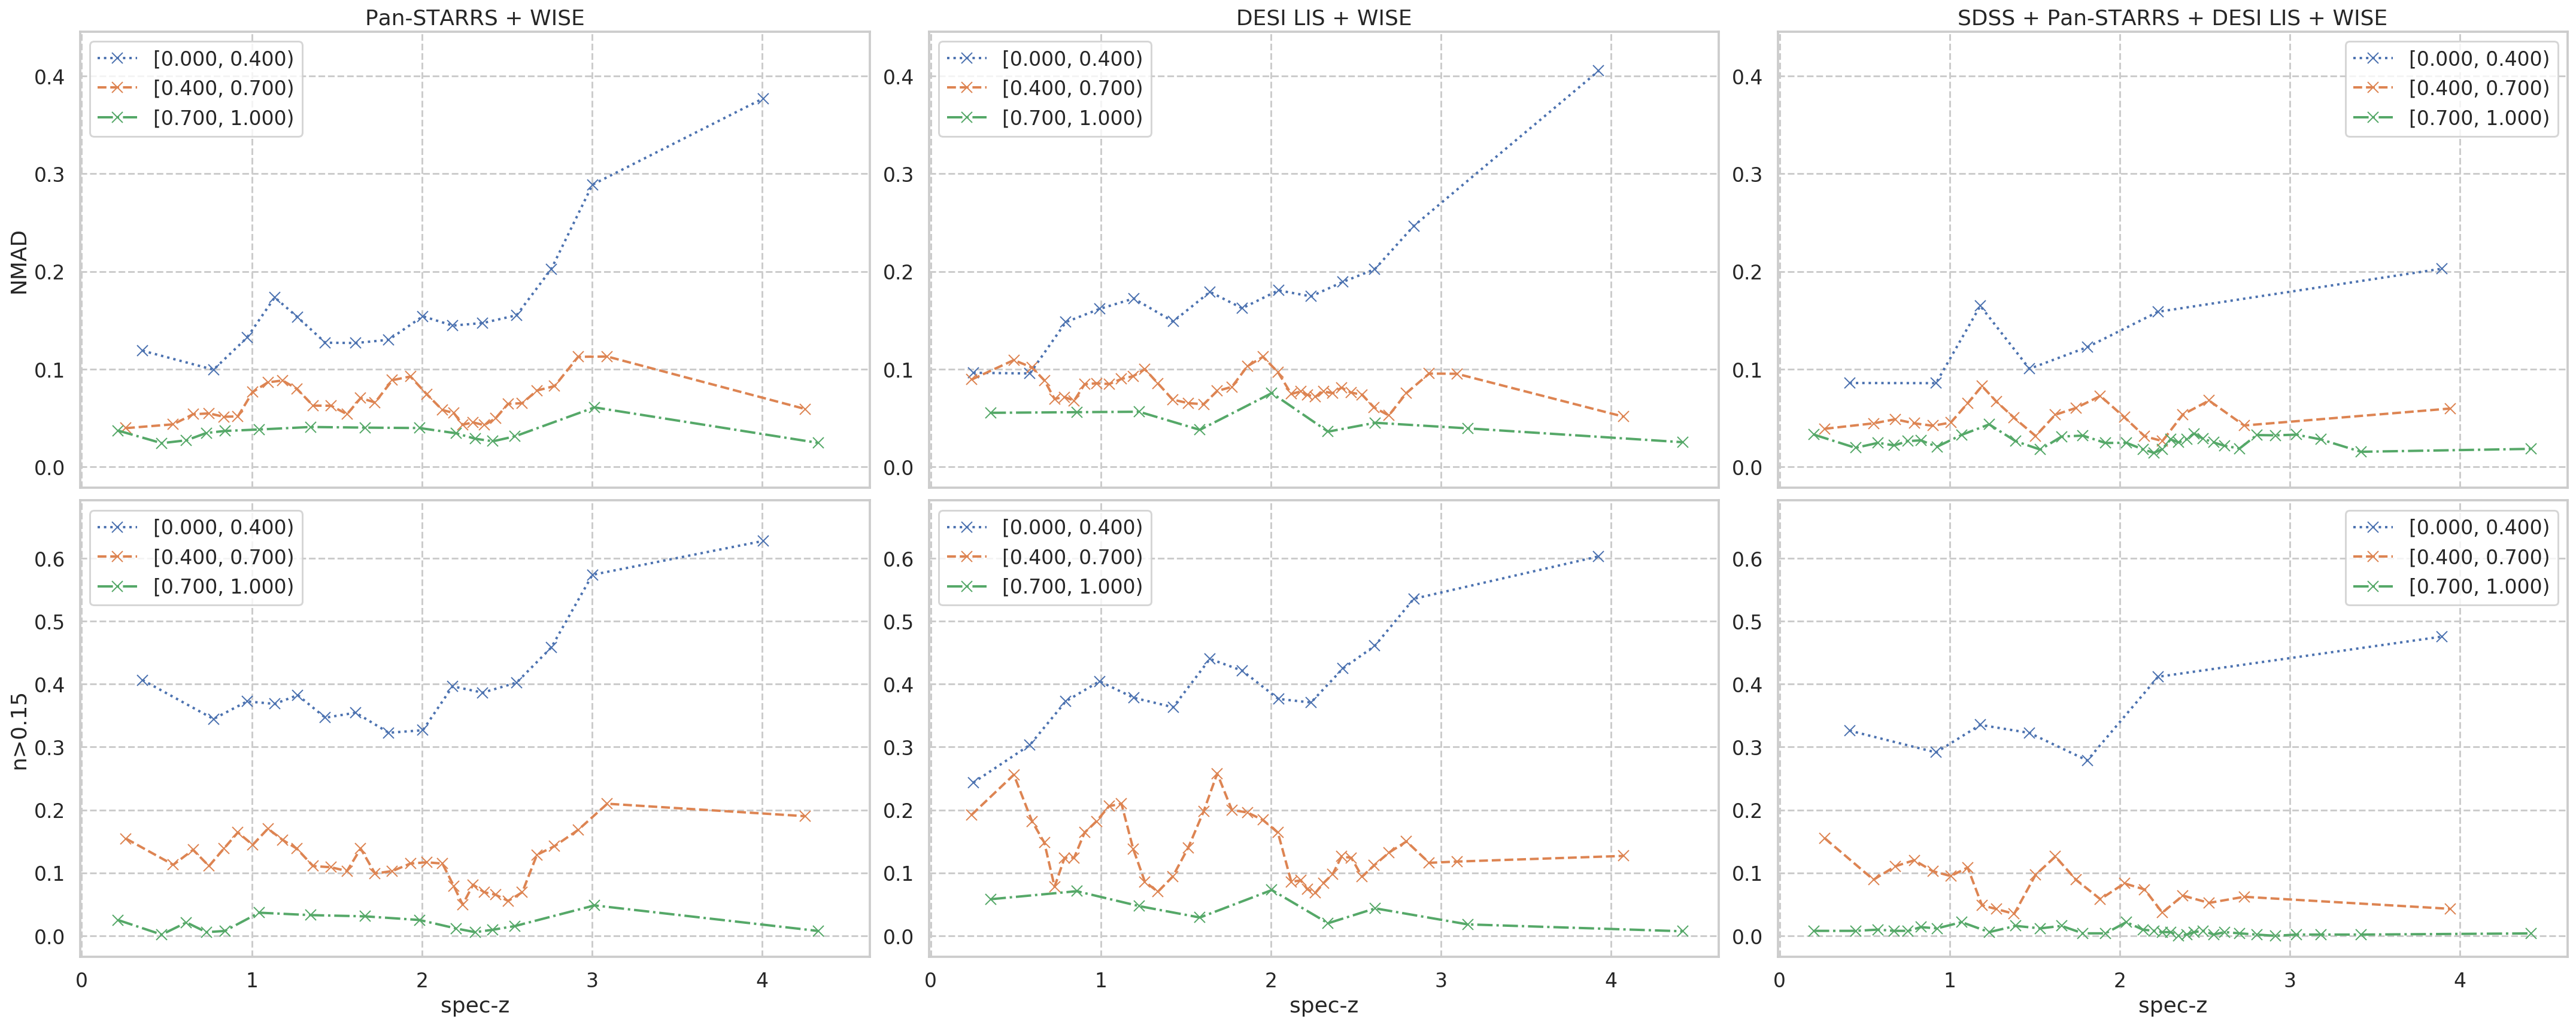
\includegraphics[width=0.9\linewidth]{images/metrics-adv-zspec-x-zconf-dr16q.png}
    \caption{Метрики в зависимости от spec-z для разных порогов по zConf на DR16q}
    \label{fig:my_label}
\end{figure}
\end{landscape}


\begin{landscape}
\begin{figure}
    \centering
    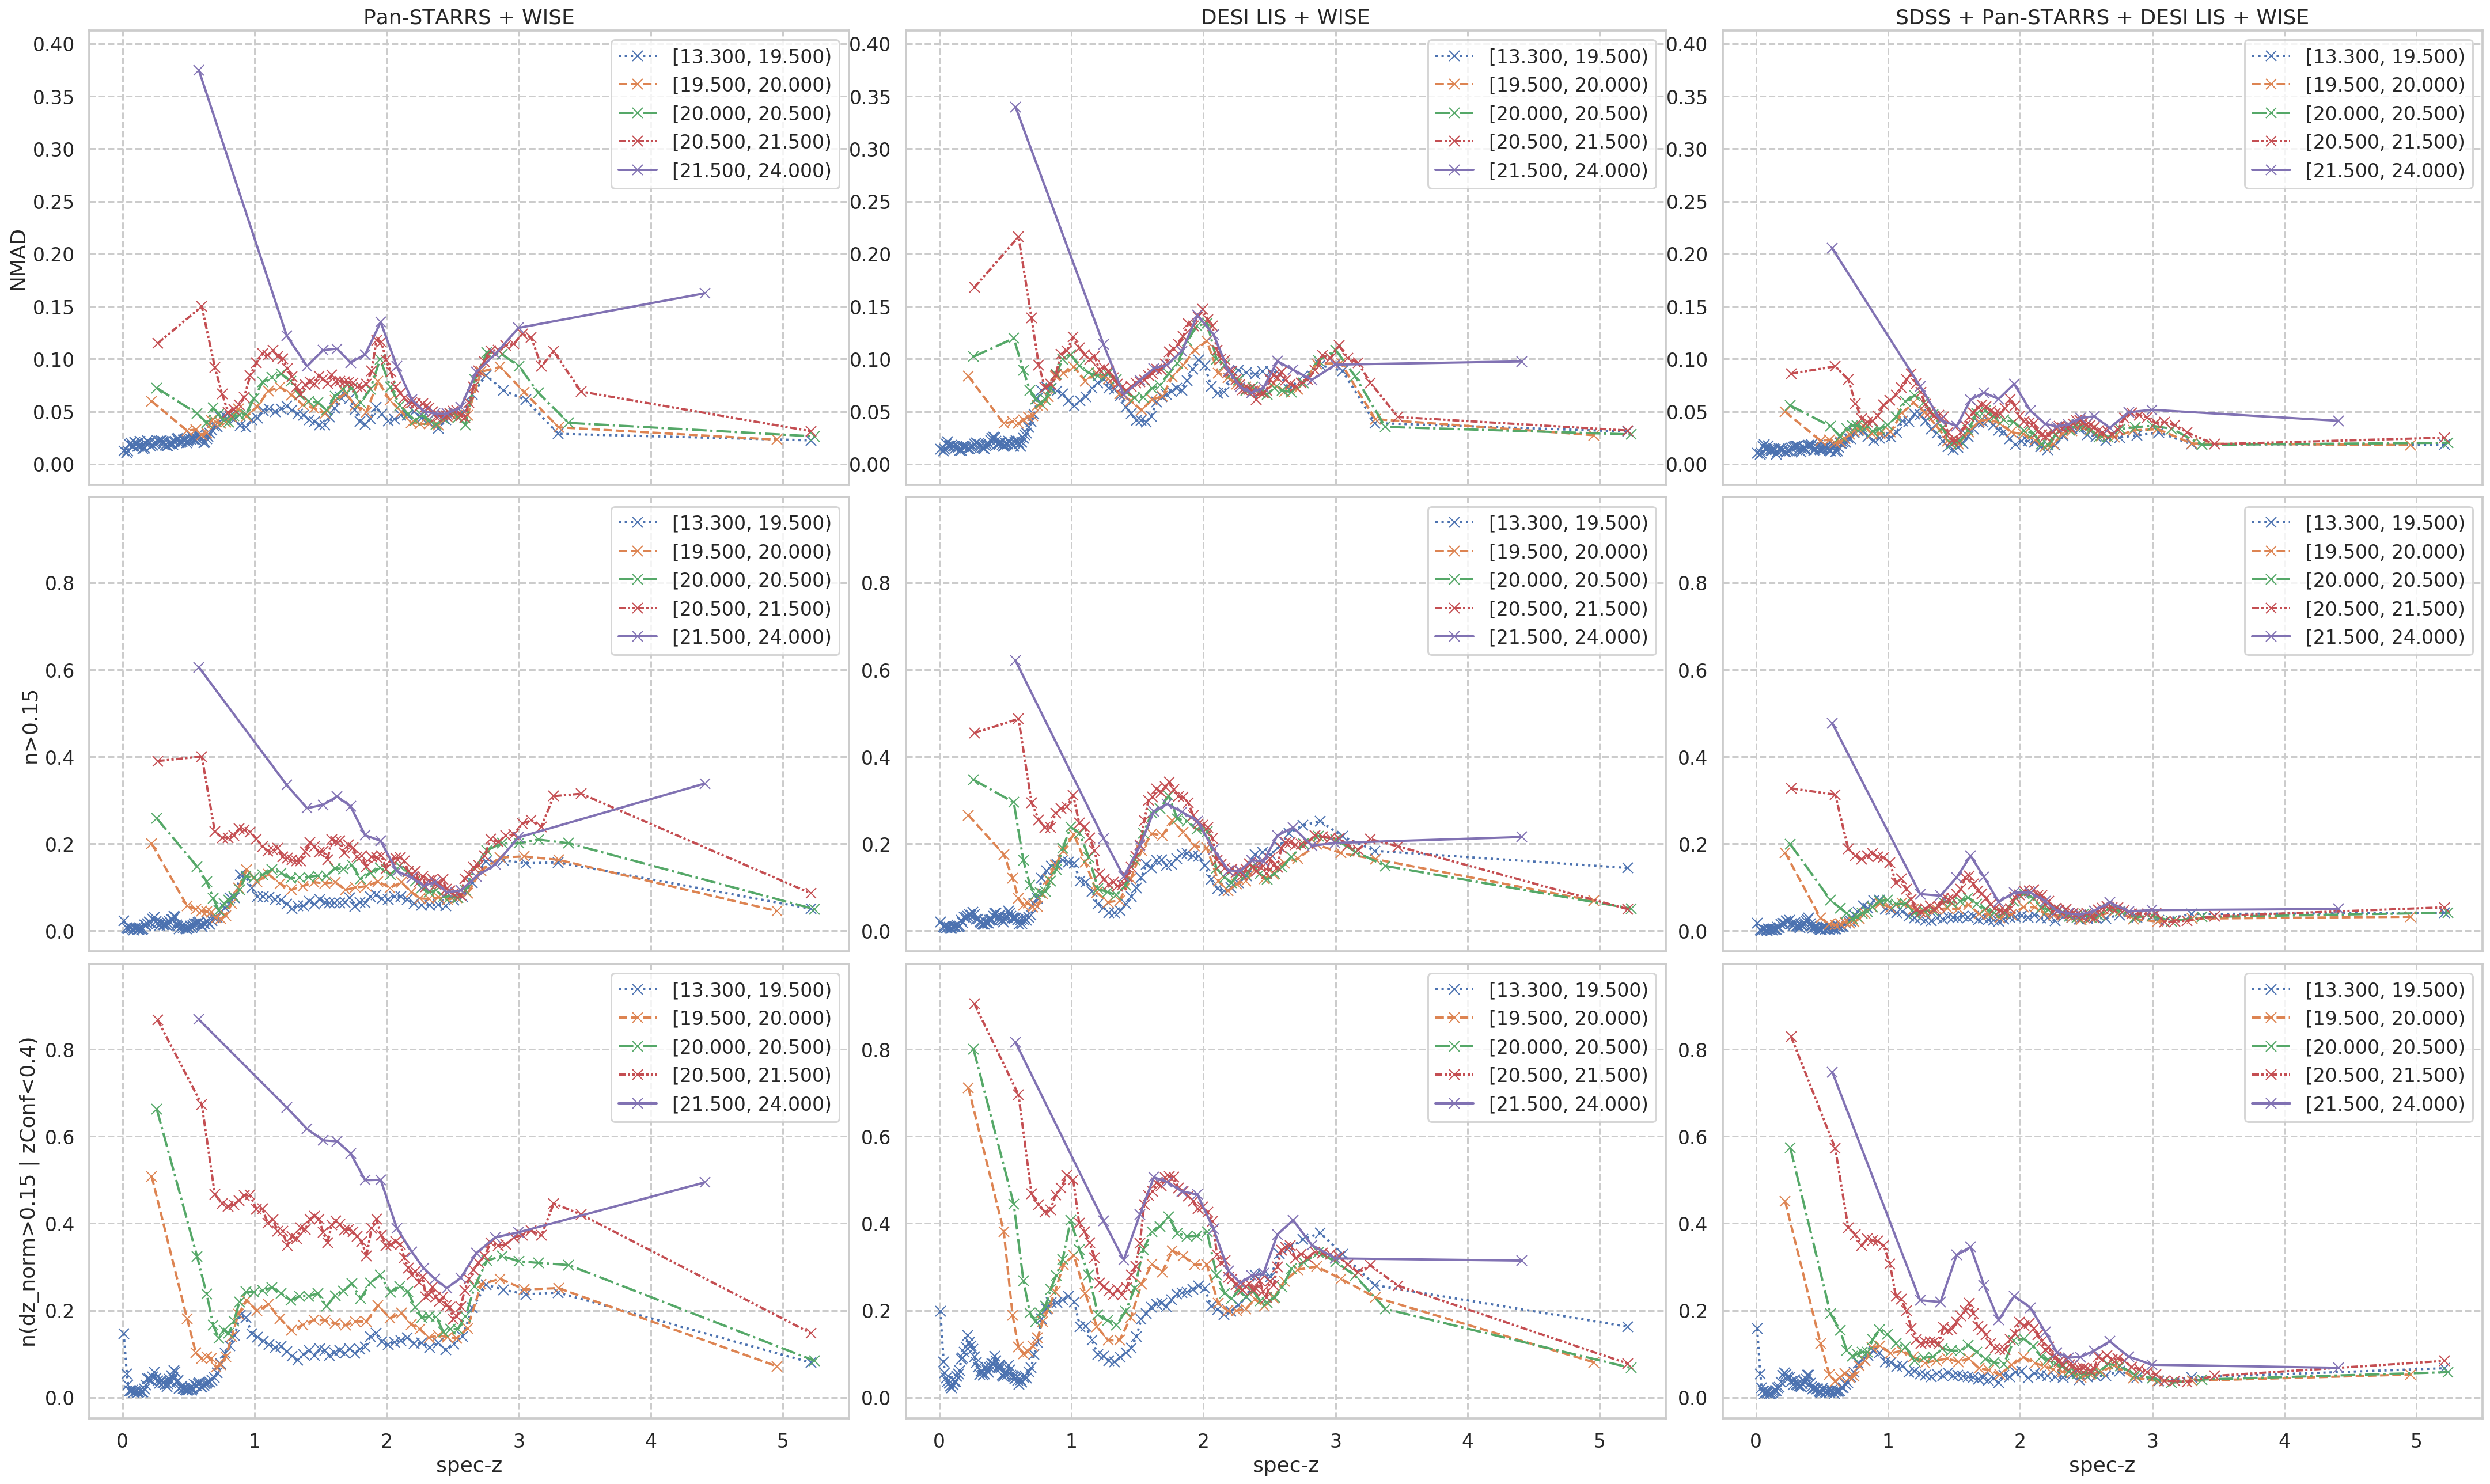
\includegraphics[width=0.9\linewidth]{images/metrics-adv-zspec-x-zmag-cv2.png}
    \caption{Метрики в зависимости от spec-z для разных порогов по $z_mag$ на кросс-валидации}
    \label{fig:my_label}
\end{figure}
\end{landscape}


\begin{landscape}
\begin{figure}
    \centering
    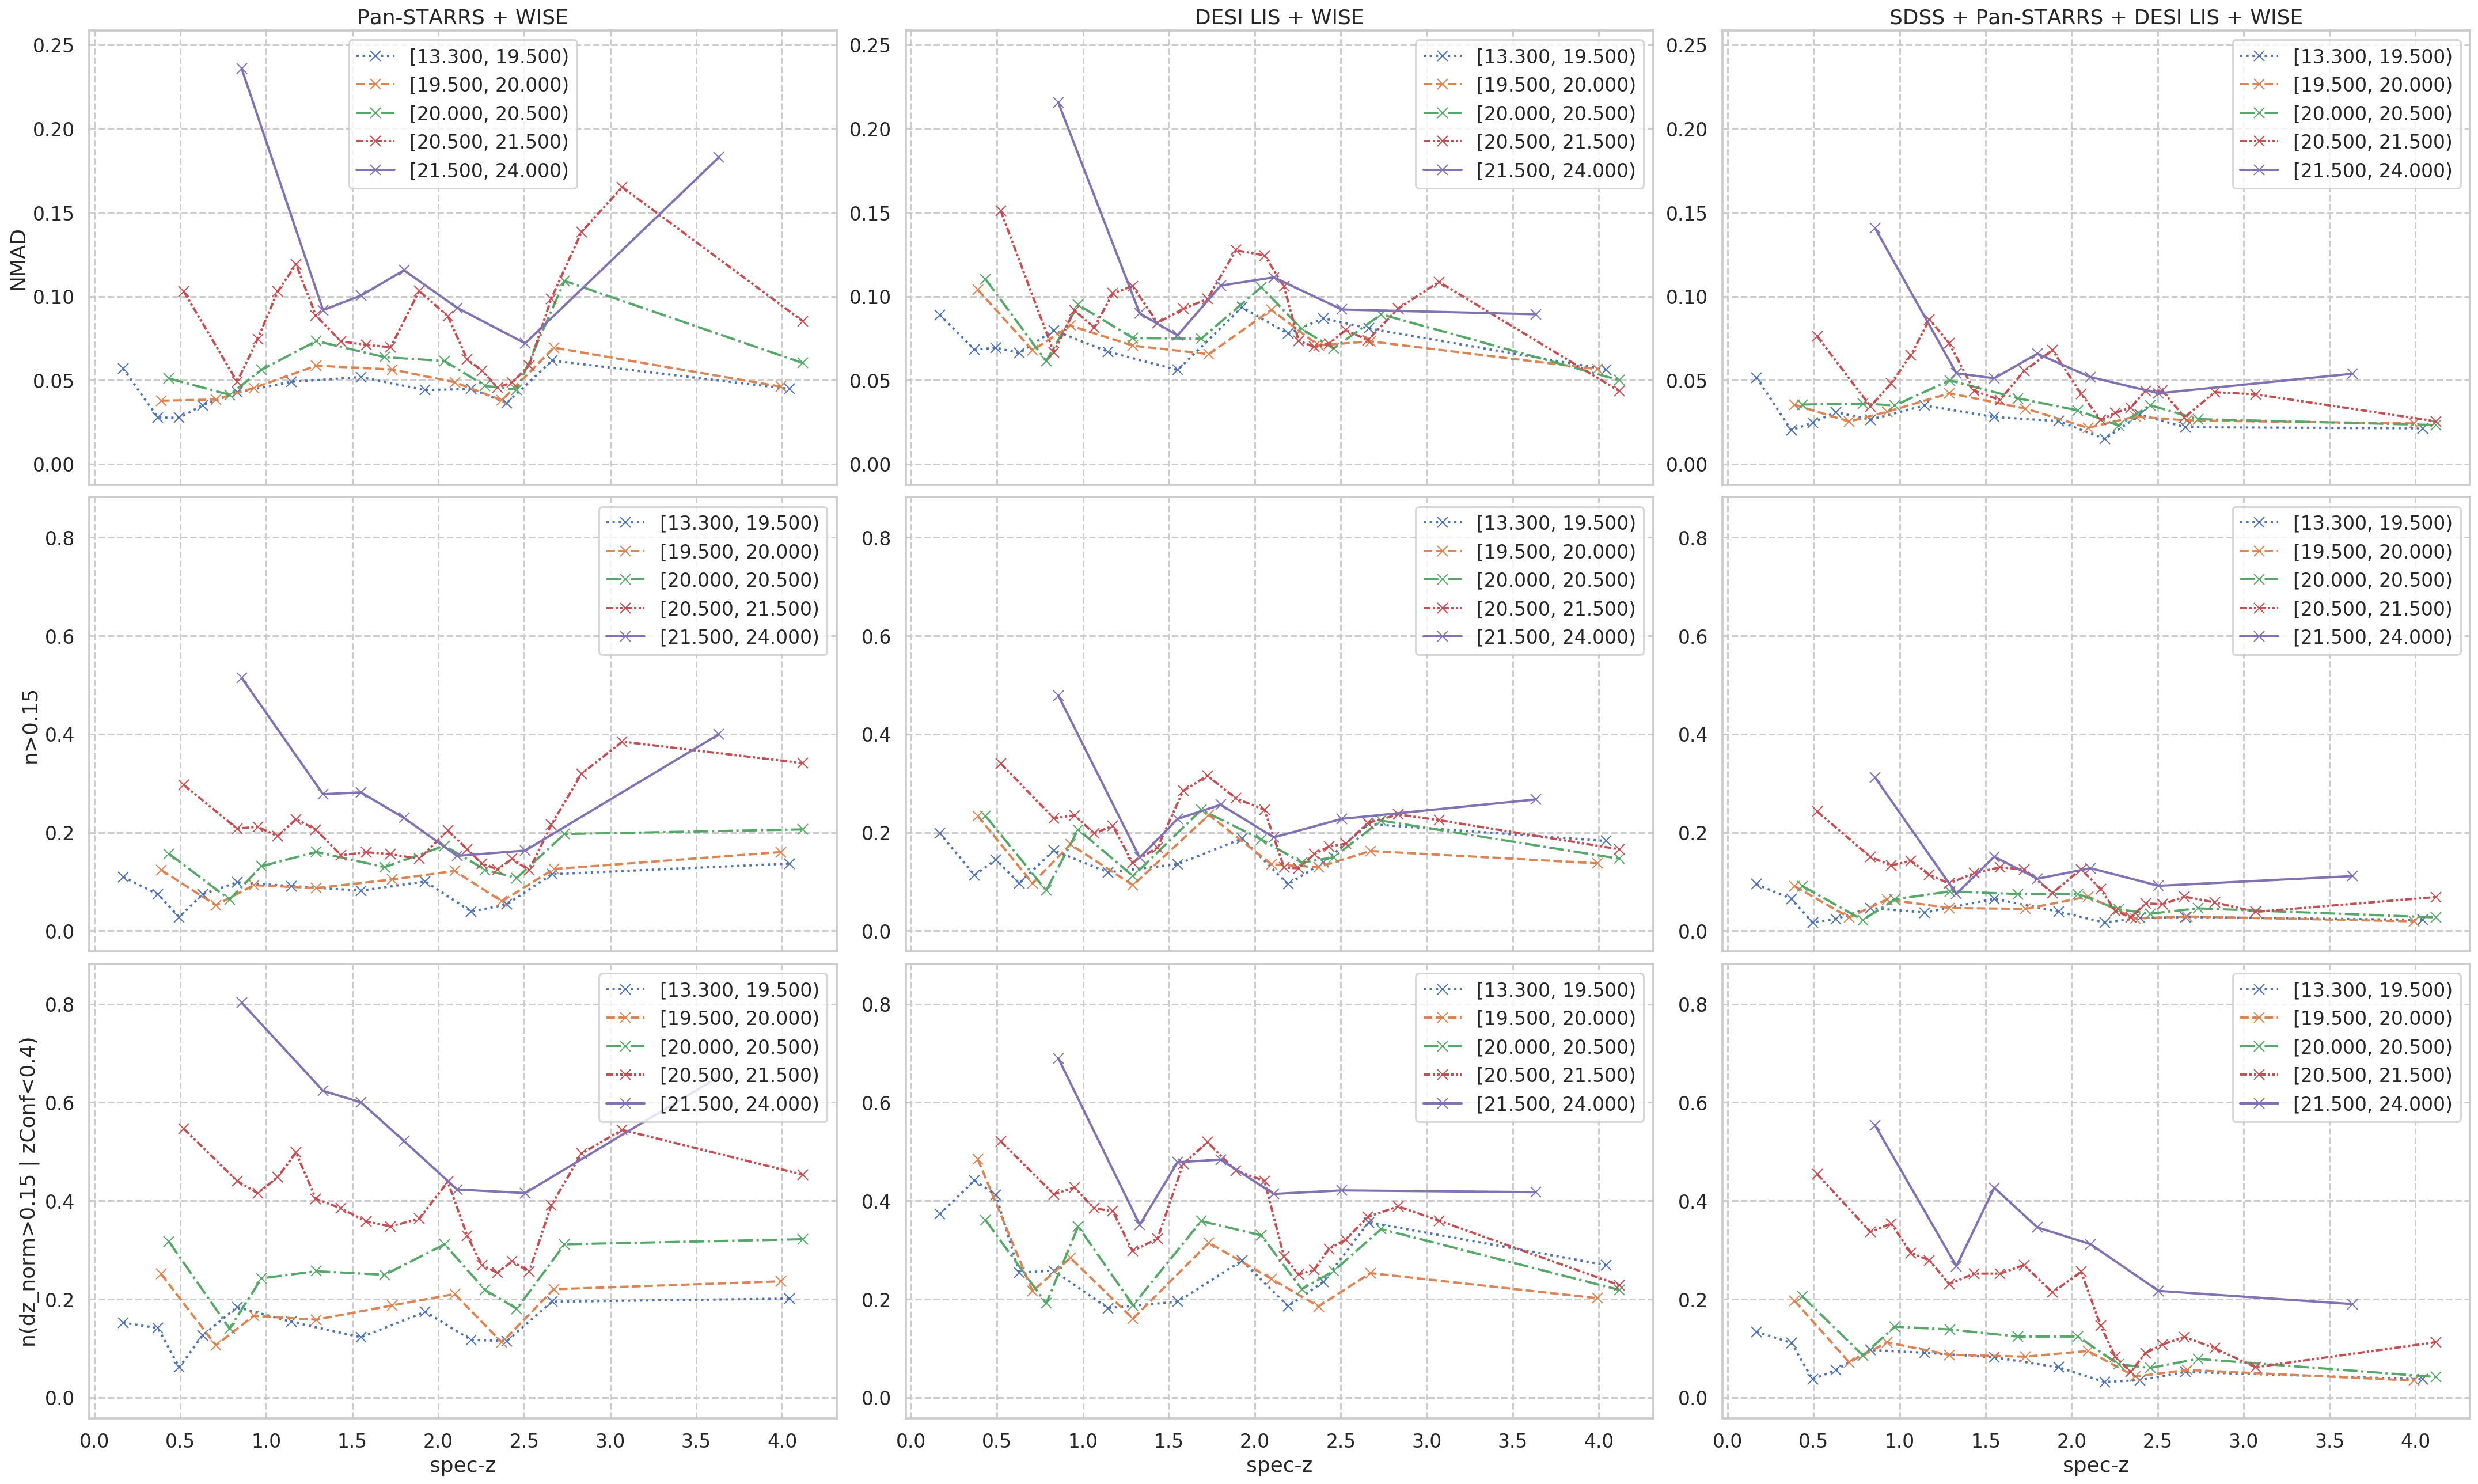
\includegraphics[width=0.9\linewidth]{images/metrics-adv-zspec-x-zmag-dr16q.png}
    \caption{Метрики в зависимости от spec-z для разных порогов по $z_mag$ на DR16q}
    \label{fig:my_label}
\end{figure}
\end{landscape}


\end{document}
